\documentclass[twoside]{report}
\usepackage[spanish,es-noshorthands]{babel}
\addto\captionsspanish{
\renewcommand{\figurename}{FIGURA}
\renewcommand{\tablename}{TABLA}
\renewcommand{\contentsname}{ÍNDICE}
}

% Document Configuration
%%%%%%%%%%%%%%%%%%%%%%%%%%%%%%%%%%%%%%%%%%%%%%%%%%%%%%%%%%%%%%%%%%%%%%

\usepackage{tabularx}
\usepackage{longtable}
\usepackage{ltxtable}
\usepackage{booktabs}
\usepackage{array}
\usepackage{collcell}
\usepackage{trimspaces}
\usepackage{multirow}
\usepackage{rotating}

%%%
%%% Formatting
%%%

% New rule type
\newcommand{\topruleb}{\midrule[\heavyrulewidth]}

% Commands to control the alignment of headers
\newcommand{\bfu}[1]{\textbf{\uppercase{#1}}}
\newcommand{\headingl}[1]{\multicolumn{1}{l}{\bfu{#1}}}
\newcommand{\headingc}[1]{\multicolumn{1}{c}{\bfu{#1}}}
\newcommand{\headingr}[1]{\multicolumn{1}{r}{\bfu{#1}}}

% Regular column types
\newcolumntype{x}{>{\collectcell\textsc}l<{\endcollectcell}}
\newcolumntype{y}{>{\collectcell\textsc}c<{\endcollectcell}}
\newcolumntype{z}{>{\collectcell\textsc}r<{\endcollectcell}}
\newcolumntype{u}{>{\collectcell\uppercase}l<{\endcollectcell}}
\newcolumntype{v}{>{\collectcell\uppercase}c<{\endcollectcell}}
\newcolumntype{w}{>{\collectcell\uppercase}r<{\endcollectcell}}
\newcolumntype{U}{>{\bfseries\collectcell\uppercase}l<{\endcollectcell}}
\newcolumntype{V}{>{\bfseries\collectcell\uppercase}c<{\endcollectcell}}
\newcolumntype{W}{>{\bfseries\collectcell\uppercase}r<{\endcollectcell}}

% Paragraph column types
\newcolumntype{L}{>{\raggedright\arraybackslash}X}
\newcolumntype{C}{>{\centering\arraybackslash}X}
\newcolumntype{R}{>{\raggedleft\arraybackslash}X}

\usepackage{xspace}
\usepackage{lipsum}
\usepackage{xcolor}

% Short verbatim can be formatted using \!text!: e.g., \!boolean!
\def\!#1!{\texttt{#1}}

% Acronyms should be placed in angled brackets: e.g., \<UML>
\def\<#1>{\lowercase{\textsc{#1}}}

% Abbreviations for references
\newcommand{\Figure}{Figure\@\xspace}
\newcommand{\Figures}{Figures\@\xspace}
\newcommand{\Table}{Table\@\xspace}
\newcommand{\Tables}{Tables\@\xspace}
\newcommand{\Section}{Section\@\xspace}
\newcommand{\Sections}{Sections\@\xspace}
\newcommand{\Appendix}{Appendix\@\xspace}
\newcommand{\Appendices}{Appendices\@\xspace}
\newcommand{\CMS}{\emph{Chana Monitoring System}\@\xspace}
\newcommand{\MI}{\textit{módulo interior}\@\xspace}
\newcommand{\MIE}{\emph{módulo interior}\@\xspace}
\newcommand{\ME}{\textit{módulo exterior}\@\xspace}
\newcommand{\MEE}{\emph{módulo exterior}\@\xspace}

% Common abbrev. are set as commands to ensure proper spacing after the dot
\newcommand{\ie}{i.e.\@\xspace}
\newcommand{\Ie}{I.e.\@\xspace}
\newcommand{\cf}{cf.\@\xspace}
\newcommand{\Cf}{Cf.\@\xspace}
\newcommand{\eg}{e.g.\@\xspace}
\newcommand{\Eg}{E.g.\@\xspace}
\newcommand{\etal}{et al.\@\xspace}
\newcommand{\etc}{etc.\@\xspace}

% Other
\newcommand{\on}{\raisebox{-1pt}{\hspace{-2pt}\textlarger[2]{$\shortmid$}}\hspace{-2pt}\@\xspace}
\newcommand{\off}{$\medcircle$\@\xspace}

% Sample text
%\newcommand{\stext}[1][1-2]{\textcolor{gray!80!red}{\lipsum[#1]}}
\newcommand{\stext}[1][1-2]{\lipsum[#1]}

% Sample paragraph
\newcommand{\spar}{\stext[1]}

% Short sample paragraph
\newcommand{\sspar}{\stext[66]}
\usepackage{enumitem}
\usepackage{relsize}
\usepackage{textcomp}
\usepackage{rotating}
\usepackage{graphbox}
\usepackage{float}
\usepackage{xfrac}
\usepackage{placeins}
\usepackage{subcaption}
\renewcommand\thesubfigure{\Alph{subfigure}}
\usepackage{wrapfig}
\usepackage{MnSymbol}
\usepackage[numbers,sort]{natbib}
\usepackage[export]{adjustbox}

\usepackage{acronym}
\renewcommand*{\aclabelfont}[1]{\textcolor{main}{#1}}
%\renewcommand*{\acsfont}[1]{\textsc{#1}}

\usepackage{url}
% Allow breaking URLs at any character
\expandafter\def\expandafter\UrlBreaks\expandafter{\UrlBreaks%
  \do\a\do\b\do\c\do\d\do\e\do\f\do\g\do\h\do\i\do\j%
  \do\k\do\l\do\m\do\n\do\o\do\p\do\q\do\r\do\s\do\t%
  \do\u\do\v\do\w\do\x\do\y\do\z\do\A\do\B\do\C\do\D%
  \do\E\do\F\do\G\do\H\do\I\do\J\do\K\do\L\do\M\do\N%
  \do\O\do\P\do\Q\do\R\do\S\do\T\do\U\do\V\do\W\do\X%
  \do\Y\do\Z}

% Allow hyphenation in texttt
\LetLtxMacro\origttfamily\ttfamily
\DeclareRobustCommand*{\ttfamily}{%
  \origttfamily
  \hyphenchar\font=`\-\relax
  \fontdimen3\font=.25em\relax
  \fontdimen4\font=.167em\relax
  \fontdimen7\font=.167em\relax
}

% Circled text
\newcommand*\circled[1]{\tikz[baseline=(char.base)]{\node[shape=circle,fill,minimum size=1.4em,inner sep=0pt] (char) {\textcolor{white}{\textbf{#1}}};}}

\newcommand*\circlefilled[1]{\tikz[baseline=(char.base)]{\node[shape=circle,fill,minimum size=1.4em,inner sep=0pt, color=#1] (char) {X}}}
\usepackage{listings}
\definecolor{gray97}{gray}{.97}
\definecolor{gray75}{gray}{.75}
\definecolor{gray45}{gray}{.45}
\definecolor{gray20}{gray}{.20}

\renewcommand\lstlistingname{LISTING}

% Default format
\lstset{
  tabsize=2,
  xleftmargin=.5cm,
  framexleftmargin=.4cm,
  keywordstyle=\color{Plum}\bfseries,
  breaklines=true,
  captionpos=t,
  basicstyle=\ttfamily\scriptsize\color{Black},
  showstringspaces=false,
  numberstyle=\ttfamily\tiny,
  numbersep=1.1cm,
  numbers=left,
  numbersep=5pt,
  showspaces=false,
  showtabs=false,
  frame=single,
  backgroundcolor=\color{gray97},
  rulesepcolor=\color{black},
  commentstyle=\color{ForestGreen}
}

% Inline OCL
\lstdefinestyle{iOCL}{language=OCL,basicstyle=\ttfamily\normalsize\color{Black}}

% QVTo
\lstdefinestyle{QVT}{language=OCL,
morekeywords={Bag, Collection, Dict, OrderedSet, Sequence, Set, Tuple, List, abstract,
access, and, any, assert, blackbox, break, case, class, collect,
collectNested, collectOne, collectselect, collectselectOne,
composes, compute, configuration, constructor, continue, datatype,
default, derived, disjuncts, do, elif, else, end, endif,
enum, except, exists, extends, exception, false, forAll, forEach ,
forOne, from, helper, if, implies, import , in, inherits, init,
inout, intermediate, invresolve, invresolveIn, invresolveone,
invresolveoneIn , isUnique, iterate, late, let, library, literal,
log, main, map, mapping, merges, metamodel, modeltype, new, not,
null, object, one, or, ordered, out, package, population, primitive, property,
query, raise, readonly, references, refines, reject, resolve, resolveIn, resolveone,
resolveoneIn, return, select, selectOne, sortedBy, static,
switch, tag, then, transformation, true, try, typedef, unlimited,
uses, var, when, where, while, with, xcollect , xmap, xor, xselect},
morecomment=[l]{//},
morecomment=[l]{--},
morecomment=[s]{/*}{*/},
stringstyle=\color{Blue},
morestring=[b]',
morestring=[b]"
}
\usepackage{tikz}
\usetikzlibrary{arrows}
\usetikzlibrary{shapes}
\usetikzlibrary{patterns}
\usetikzlibrary{positioning}
\usetikzlibrary{calc}
\usetikzlibrary{trees}

\newcommand*{\stereotype}[1]{
  <<{#1}>>
}

\newcommand*{\datatype}[1]{
  \stereotype{datatype}\\
  #1
}

\newcommand*{\enum}[1]{
  \stereotype{enumeration}\\
  #1
}

\newcommand*{\obj}[2]{
  \underline{{#1}~:~{#2}}
}

\newcommand*{\attributes}[1]{
  \nodepart{second}
  \begin{tabular}{@{}l@{}}
  #1
  \end{tabular}
}

\newcommand*{\literals}[1]{
  \nodepart{second}
  \ttfamily
  \begin{tabular}{@{}l@{}}
  #1
  \end{tabular}
}

\newcommand*{\operations}[1]{
  \nodepart{third}
  \begin{tabular}{@{}l@{}}
  #1
  \end{tabular}
}

\tikzstyle{reportcolor}=[
  draw=black,
  line width = 0.4pt
]

\tikzstyle{box}=[
  reportcolor,
  rectangle,
  align=center,
  minimum width=5em
]

\tikzstyle{abstractbox}=[box,
  every text node part/.style={
    font=\itshape
  }
]

\tikzstyle{class}=[box,
  rectangle split,
  rectangle split parts=2,
  minimum width=9em,
  rectangle split part align={center, left}
]

\tikzstyle{classop}=[class,
  rectangle split parts=3,
  rectangle split part align={center, left, left}
]
  
\tikzstyle{object}=[class]

\tikzstyle{abstractclass}=[class,
  every text node part/.style={
    font=\itshape
  }
]

\tikzstyle{enum}=[class]

\tikzstyle{datatype}=[class]

\tikzstyle{inherits}=[reportcolor, ->, > = open triangle 90]

\tikzstyle{contains}=[reportcolor, diamond->, > = angle 45]

\tikzstyle{assoc}=[reportcolor, ->, > = angle 45]

\tikzstyle{biassoc}=[reportcolor, <->, > = angle 45]



\usepackage{xcolor}
\usepackage{ifthen}
\usepackage{tabto}
\usepackage[page]{pagenote}
\makepagenote

\newlength\cindent
\setlength\cindent{1.5em}
\renewcommand{\notesname}{\uppercase{Notes for Clarifications}}
\renewcommand*{\notedivision}{\section*{\notesname}}
\renewcommand*{\sectionname}{\uppercase{Section}}
\renewcommand{\notenumintext}[1]{\textsuperscript{\textcolor{red}{#1}}}
\renewcommand{\thepagenote}{\roman{pagenote}}
\renewcommand{\prenoteinnotes}{\par\hangindent=\cindent\hangafter=1\noindent}
\renewcommand{\postnoteinnotes}{\par}
\renewcommand{\noteentry}[4]{%
\prenoteinnotes
\noteidinnotes{#1}{#2}%
\tabto{\cindent}%
\noteinnotes{#3}\dotfill%
\textcolor{main}{\pageinnotes{#4}}%
\vspace{6pt}
\postnoteinnotes}

\makeatletter
\def\blankfootnote{\xdef\@thefnmark{}\@footnotetext}
\makeatother



\newcommand{\clarify}[2]{%
  {\color{red}%
      #1%
    \ifthenelse{\equal{#2}{}}{%
    }{%
      \addtocounter{pagenote}{1}%
      \blankfootnote{\color{red}\textsuperscript{\thepagenote}~#2}%
      \addtocounter{pagenote}{-1}%
    }%
  }%
  \ifthenelse{\equal{#1}{}}{%
    \ifthenelse{\equal{#2}{}}{%
    }{%
      \pagenote{#2}%
    }%
  }{%
    \ifthenelse{\equal{#2}{}}{%
      \pagenote{\textcolor{main}{#1}}%
    }{%
      \pagenote{\textcolor{main}{#1} --- #2}%
    }%
  }%
}

% Document Configuration
%%%%%%%%%%%%%%%%%%%%%%%%%%%%%%%%%%%%%%%%%%%%%%%%%%%%%%%%%%%%%%%%%%%%%%

\title{%
  Chana Monitoring System%
}

\author{
  Abel Gómez
}
\subtitlea{
  Manual de usuario
}
\subtitleb{
  Versión 1.0
}
\date{
  \today
}
\cover{
  images/template/cover
}
\back{
  images/template/back
}
\copyrightnotice{Abel Gómez}

% Begin document
%%%%%%%%%%%%%%%%%%%%%%%%%%%%%%%%%%%%%%%%%%%%%%%%%%%%%%%%%%%%%%%%%%%%%%

\begin{document}

% Title page
\maketitle

% Table of Contents
\tableofcontents

% Acronyms
%\section*{List of Acronyms}
\markboth{\uppercase{Acronyms}}{\uppercase{Acronyms}}

\begin{acronym}[AAAAAA]
  \acro{TIAEA}{This is an Example Acronym}
  \acro{TIAnEA}{This is Another Example Acronym}
  \acro{TIYAEA}{This is yet Another Example Acronym}
  \acro{CTAN}{Comprehensive \TeX\ Archive Network}
\end{acronym}

% Contents
\section{El \textit{Chana Monitoring System}}
\label{sect:intro}

El \CMS consta de dos módulos que se comunican a través de una conexión wifi estándar: el \MIE y el \MEE.

\begingroup

\setlength{\columnsep}{6pt}
\setlength{\intextsep}{6pt}

\begin{wrapfigure}{o}{0.5\columnwidth}
  \centering
  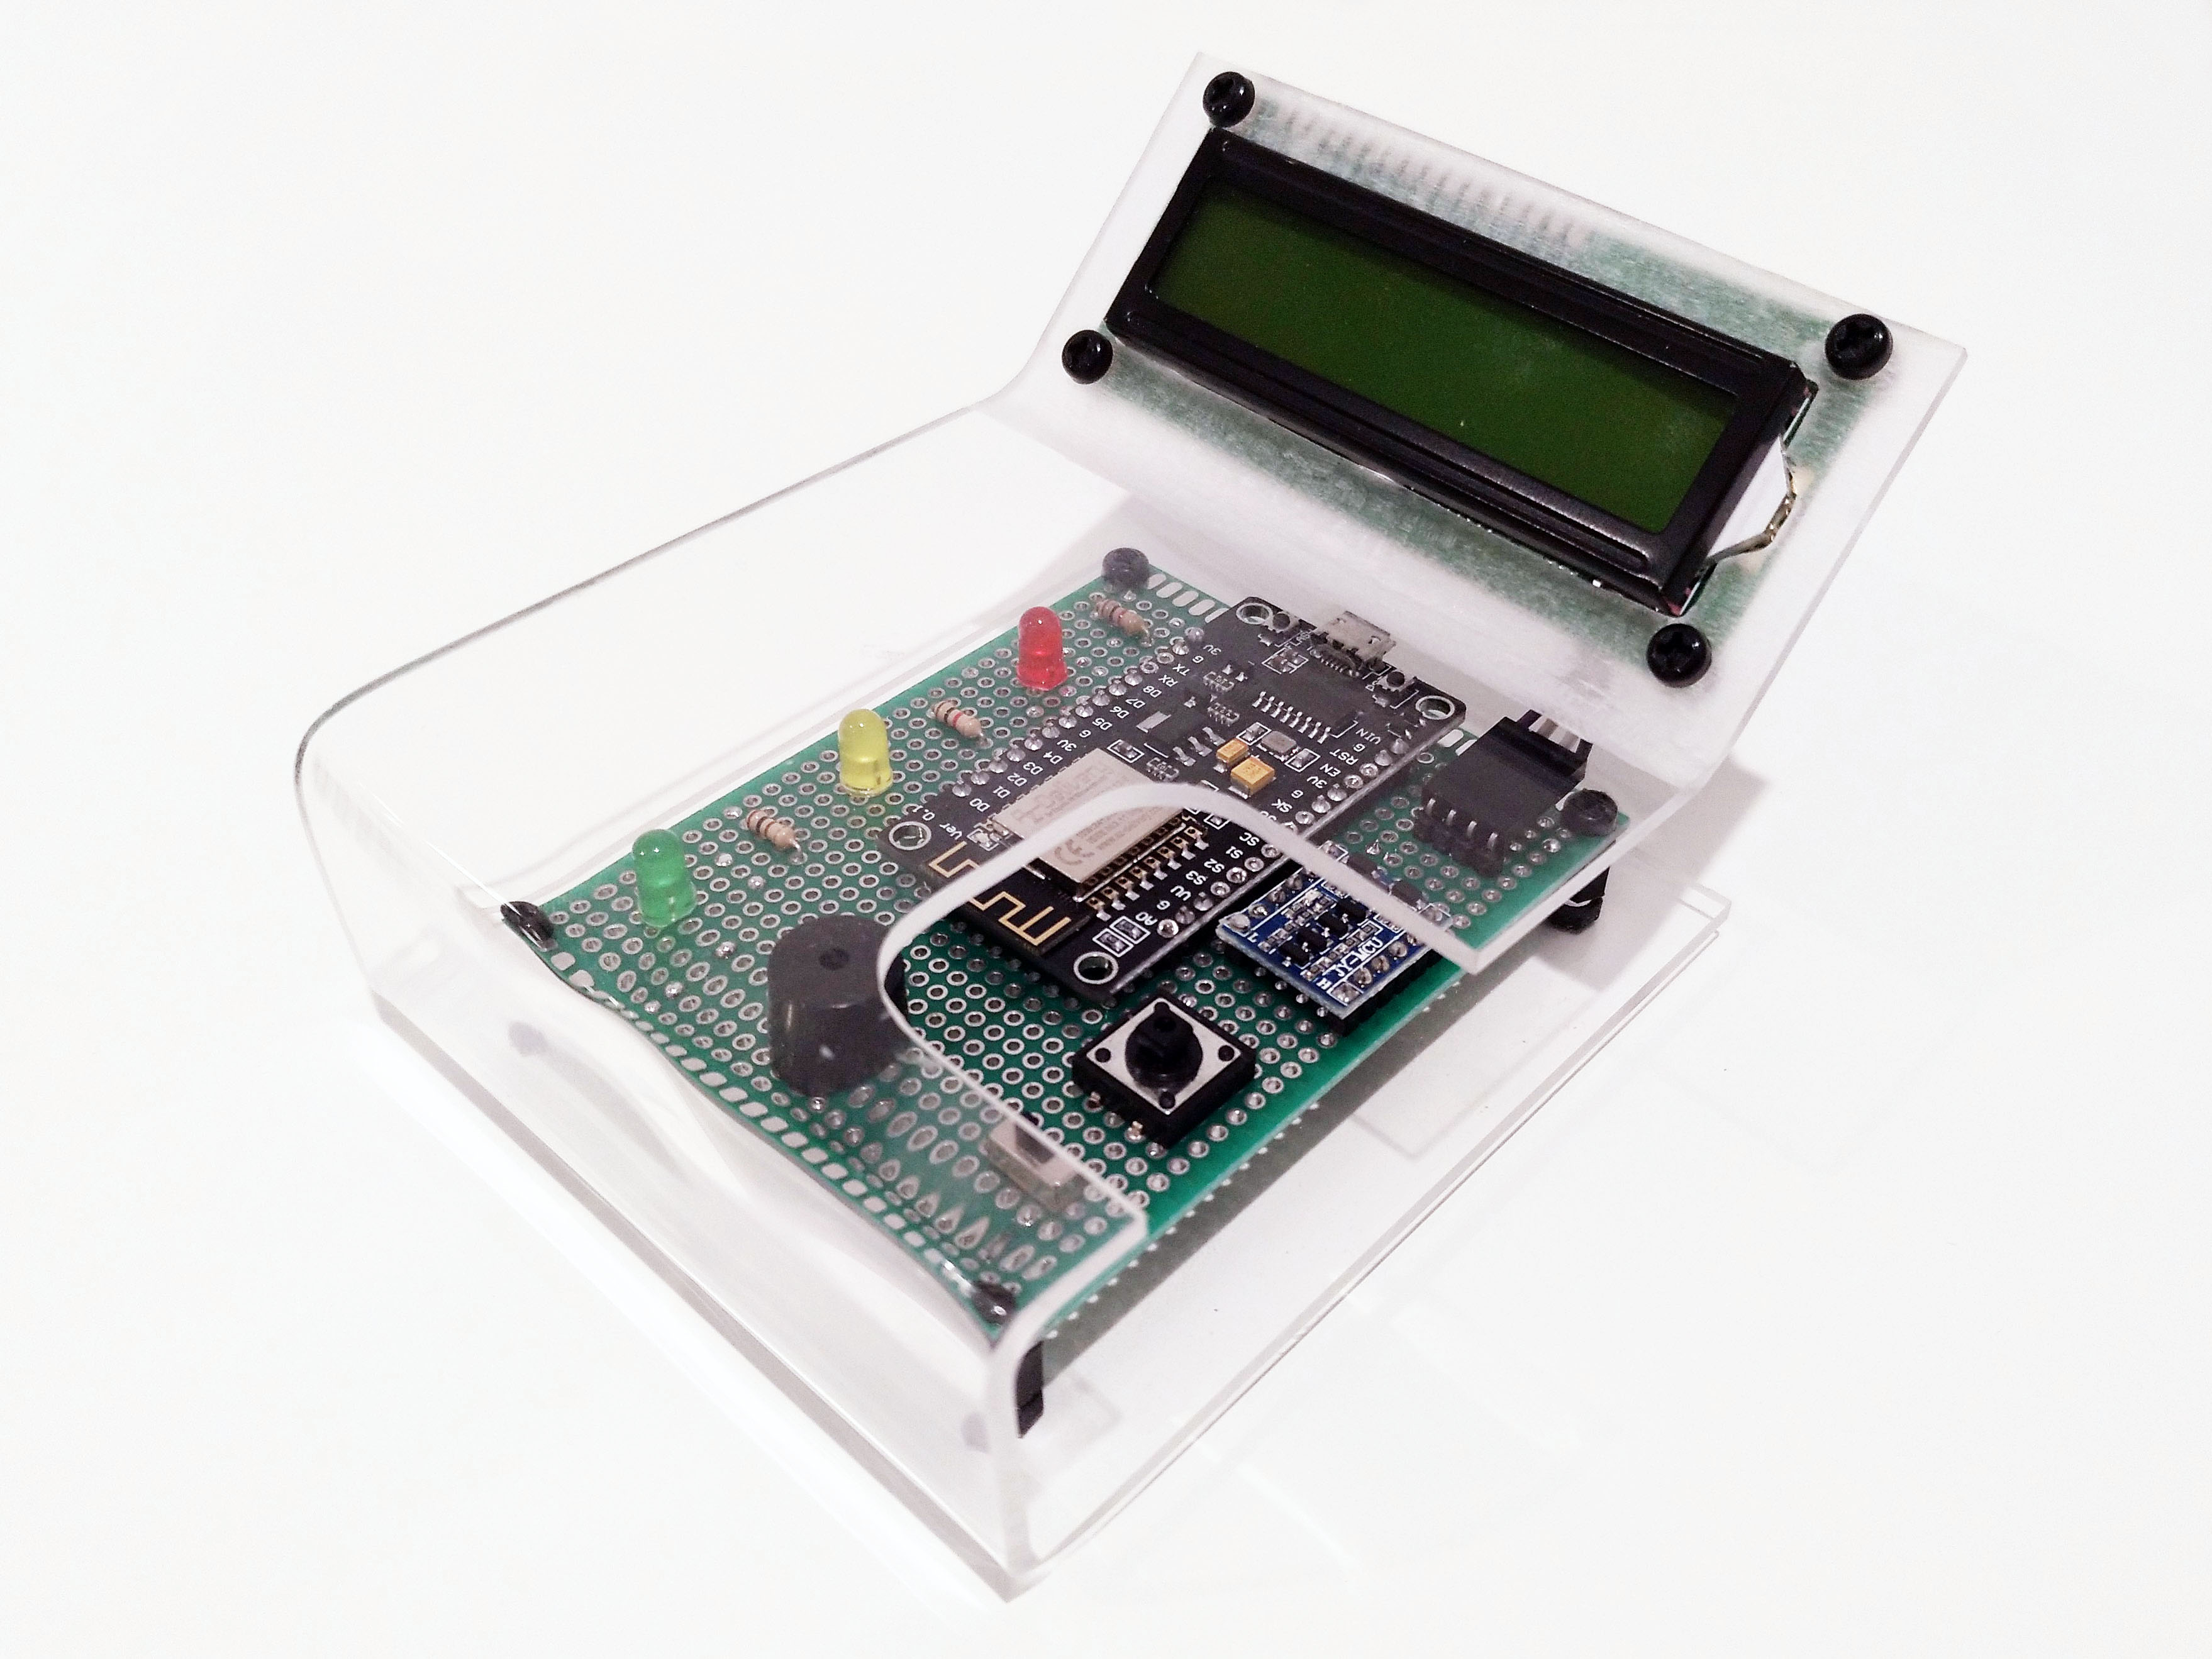
\includegraphics[width=0.5\columnwidth]{../photos/interior.jpg}
  \caption{Módulo interior}
  \label{fig:interior}
\end{wrapfigure}

El \MIE se debe colocar en el interior del hogar, preferiblemente en la habitación donde se encuentra la unidad interior de aire acondicionado que se desea monitorizar.
El \MI proporciona la información transmitida por el \ME, que monitoriza el estado del depósito de la unidad de aire acondicionado exterior, así como del ambiente exterior (temperatura y humedad).
En caso de que el depósito se llene o se produca algún fallo, será el \MI el que lanzará los distintos avisos o alarmas a través de la pantalla, los testigos de colores, y la alarma sonora.
El \MI se alimenta mediante un adaptador de corriente USB estándar.

\begin{wrapfigure}[12]{o}{0.5\columnwidth}
  \centering
  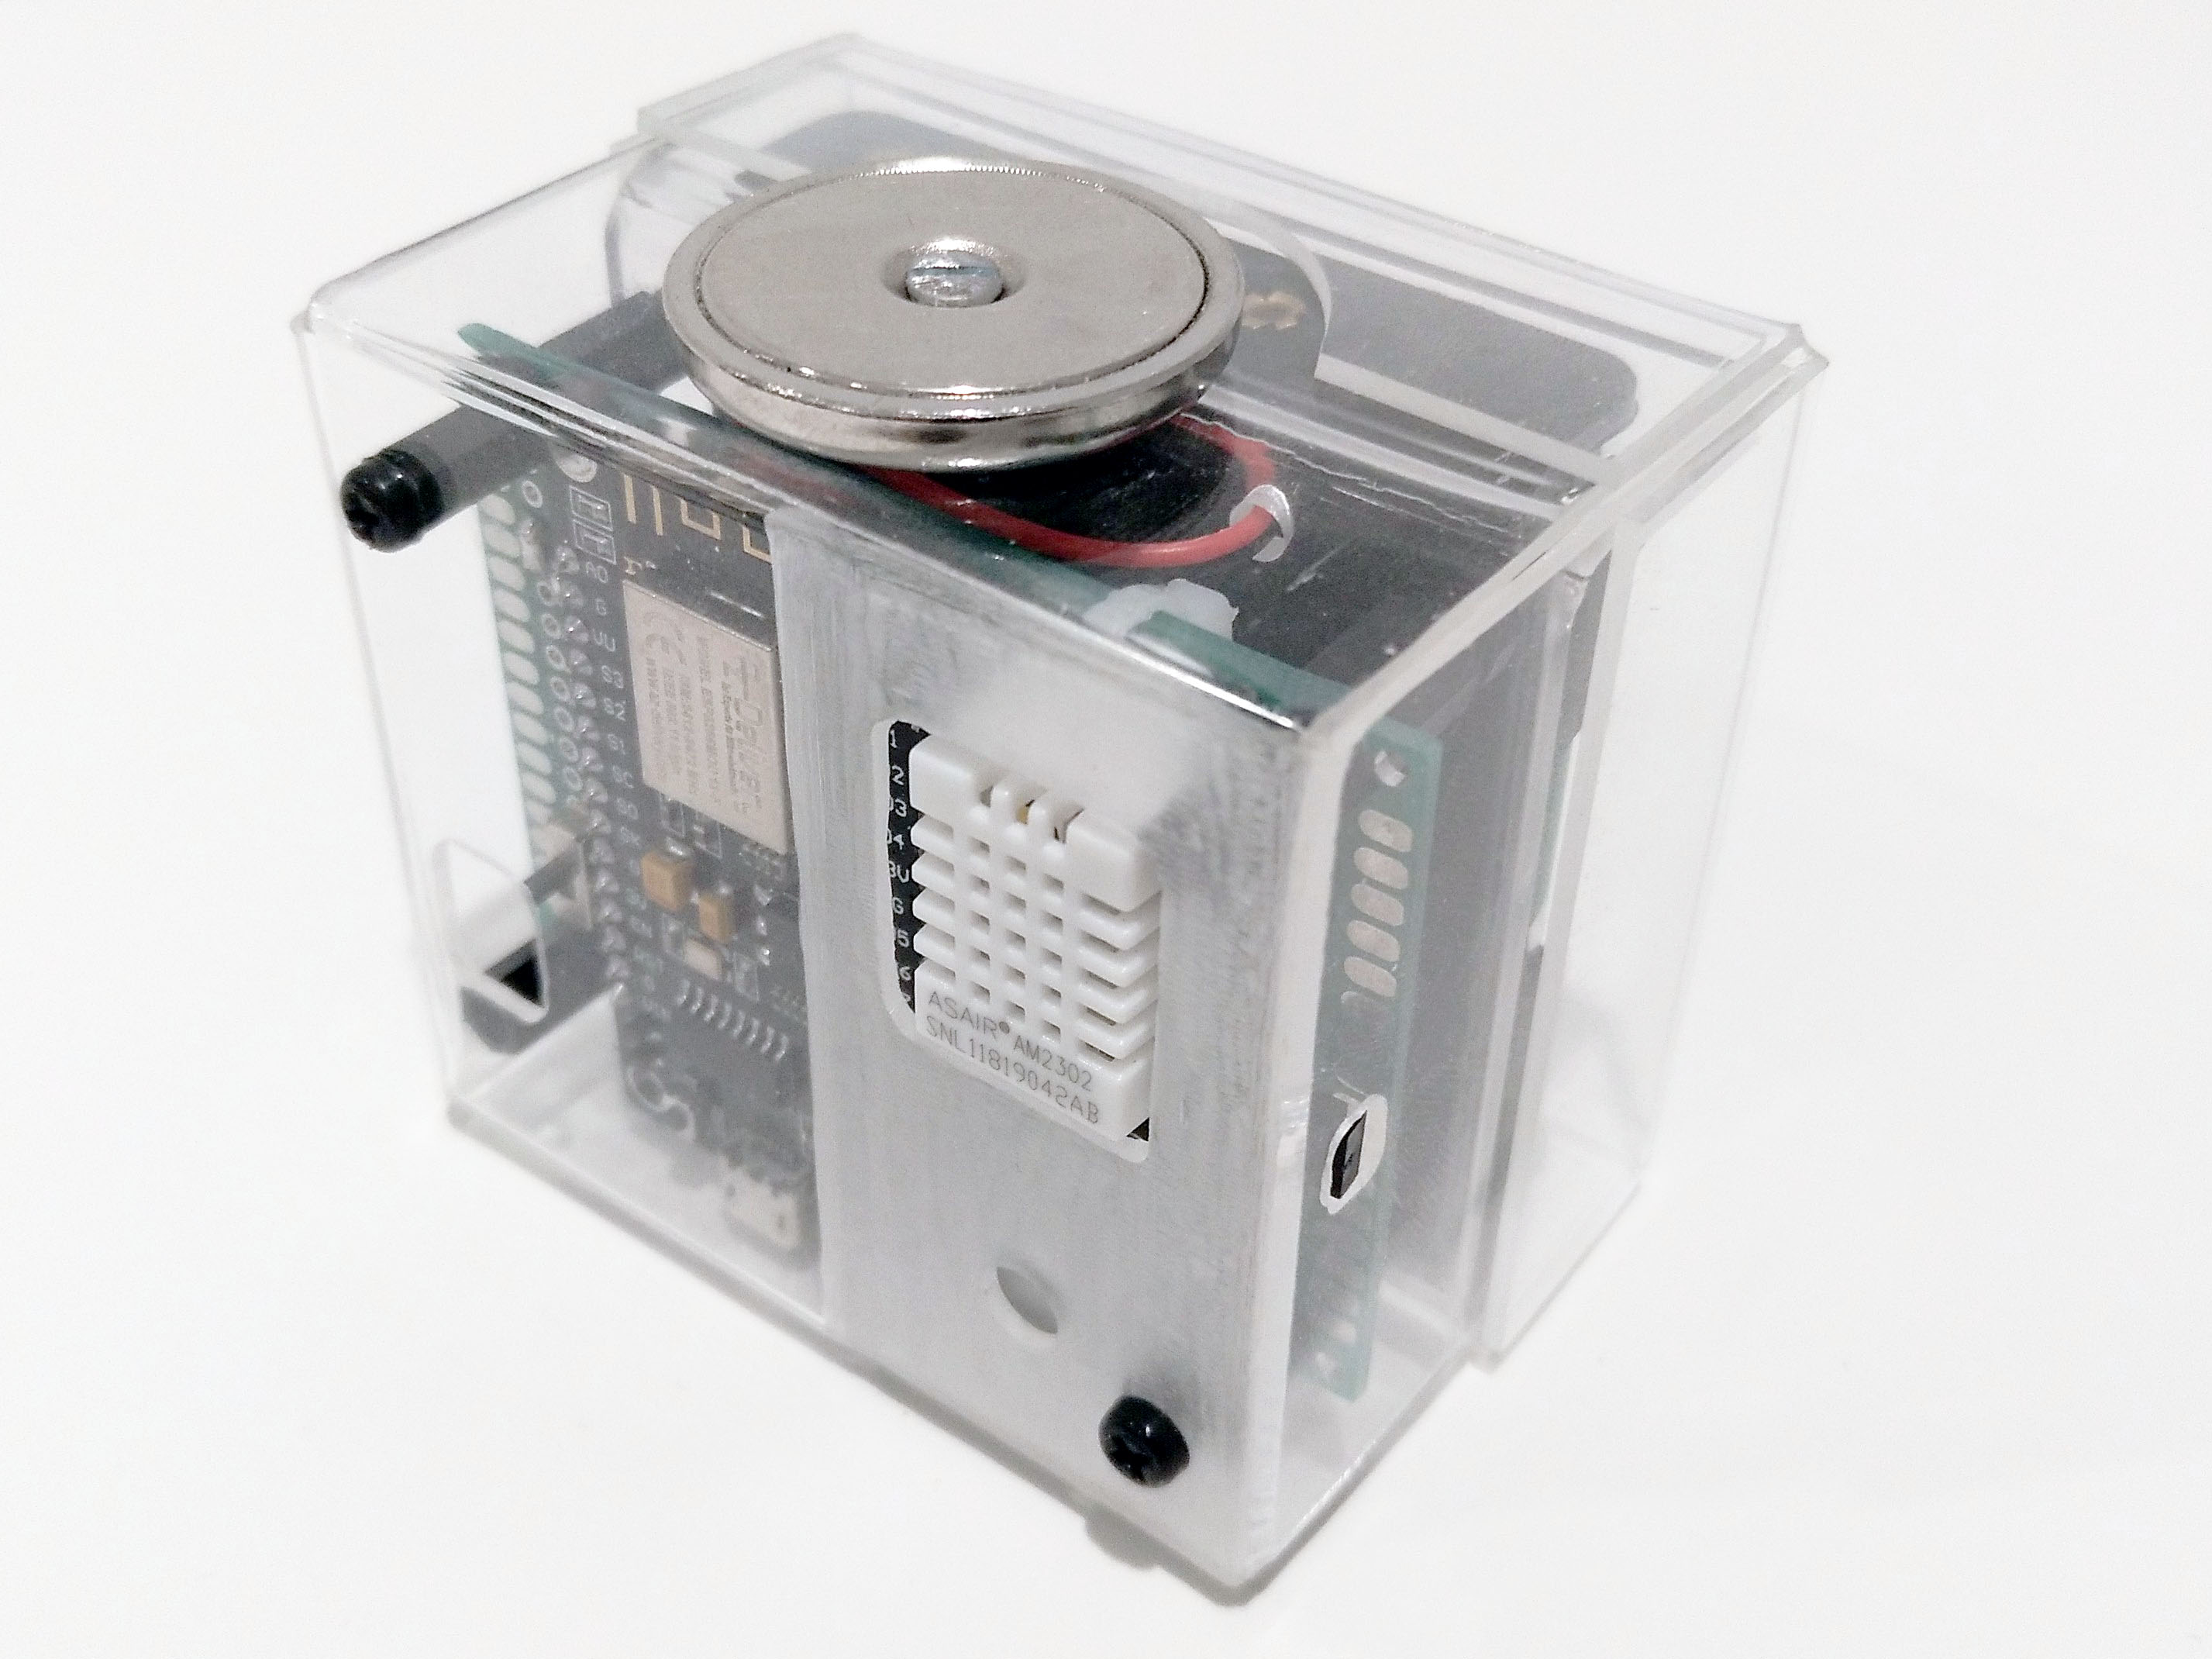
\includegraphics[width=0.5\columnwidth]{../photos/exterior.jpg}
  \caption{Módulo exterior}
  \label{fig:exterior}
\end{wrapfigure}

El \MEE recoge información mediante diferentes sensores, como el interruptor de flotador que debe introducirse dentro del depósito de agua a monitorizar.
Debe colocarse cerca de la unidad exterior de aire acondicionado en un lugar ventilado, alejado de la luz solar directa y del agua de lluvia.
El \ME dispone de un imán que permite fijarlo a la carcasa de la unidad exterior de aire acondicionado fácilmente.
El \MEE se alimenta mediante 4 pilas AA recargables de NiMH.

\importantbegin{No emplear pilas alcalinas}
El \MEE no se puede alimentar con pilas alcalinas estándares ya que proporcionan una tensión de salida de 1,5 V. \textbf{Siempre se han de emplear 4 pilas AA recargables de NiMH} (que dan una tensión de salida de 1,2 V durante la mayor parte de su vida útil). El empleo de pilas alcalinas puede provocar daños permanentes por sobretensión en el \ME. 
\importantend

\endgroup

\subsection{Controles}
\label{sect:controles}

La figura~\ref{fig:interior-controls} muestra los principales controles del \MI:


\begin{enumeratecompact}
  \item[\textbf{\color{main}I1}:] Pantalla LCD.
  \item[\textbf{\color{main}I2}:] Luz de notificación de fallo.
  \item[\textbf{\color{main}I3}:] Luz de notificación de configuración.
  \item[\textbf{\color{main}I4}:] Luz de notificación de conexión.
  \item[\textbf{\color{main}I5}:] Botón de reinicio.
  \item[\textbf{\color{main}I6}:] Conexión de alimentación USB.
  \item[\textbf{\color{main}I7}:] Luz de notificación de actividad.
  \item[\textbf{\color{main}I8}:] Botón multiuso.
  \item[\textbf{\color{main}I9}:] Interruptor de la alarma sonora (\on = encendido, \off = apagado).
  \item[\textbf{\color{main}I10}:] Emisor de alarma sonora.
\end{enumeratecompact}

\begin{figure}
  \centering
  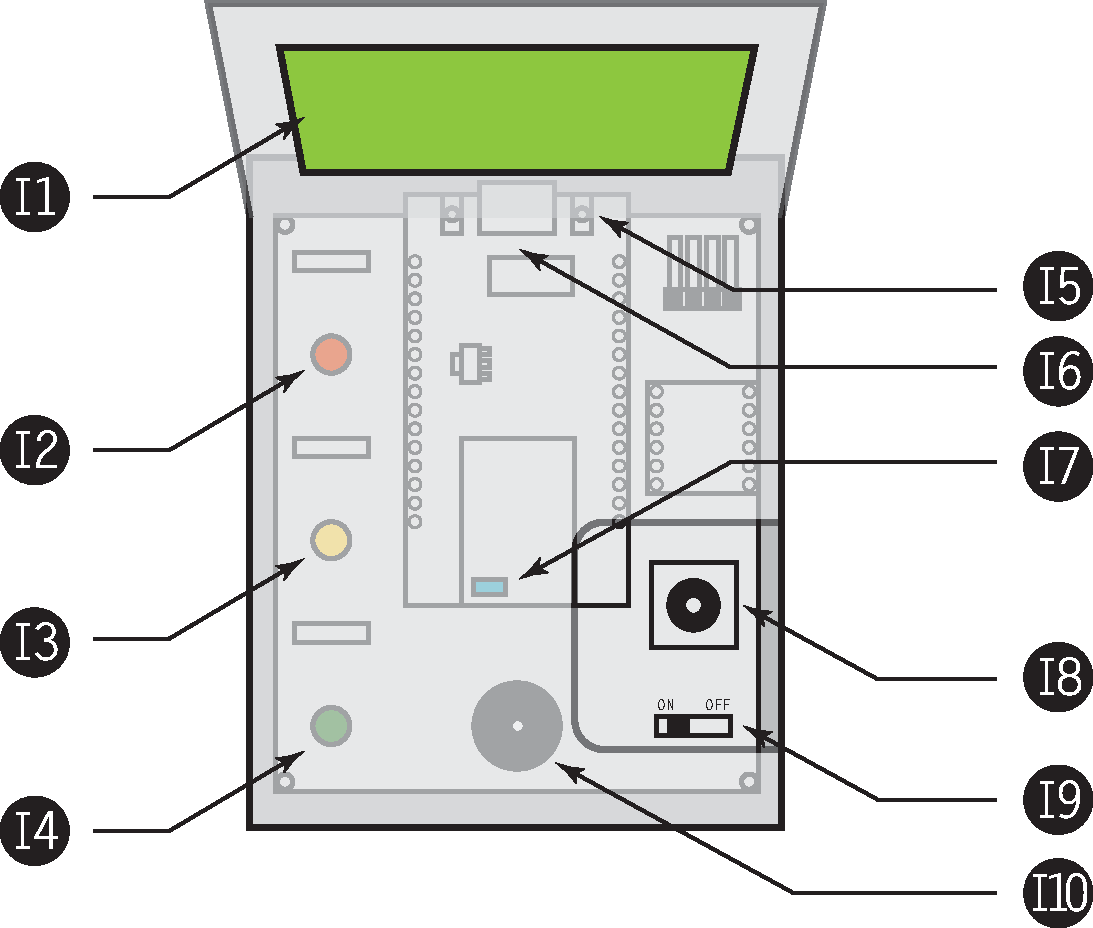
\includegraphics[width=0.8\columnwidth]{../design/interior-controls}
  \caption{Controles del módulo interior}
  \label{fig:interior-controls}
\end{figure}

La figura~\ref{fig:exterior-controls} muestra los principales controles del \ME:

\begin{enumeratecompact}
  \item[\textbf{\color{main}E1}:] Luz de notificación de actividad.
  \item[\textbf{\color{main}E2}:] Interruptor de encendido (\on = encendido, \off = apagado).
  \item[\textbf{\color{main}E3}:] Sensor de temperatura y humedad.
  \item[\textbf{\color{main}E4}:] Conexión para interruptor de flotador.
  \item[\textbf{\color{main}E5}:] Botón de configuración.
\end{enumeratecompact}

\begin{figure}
  \centering
  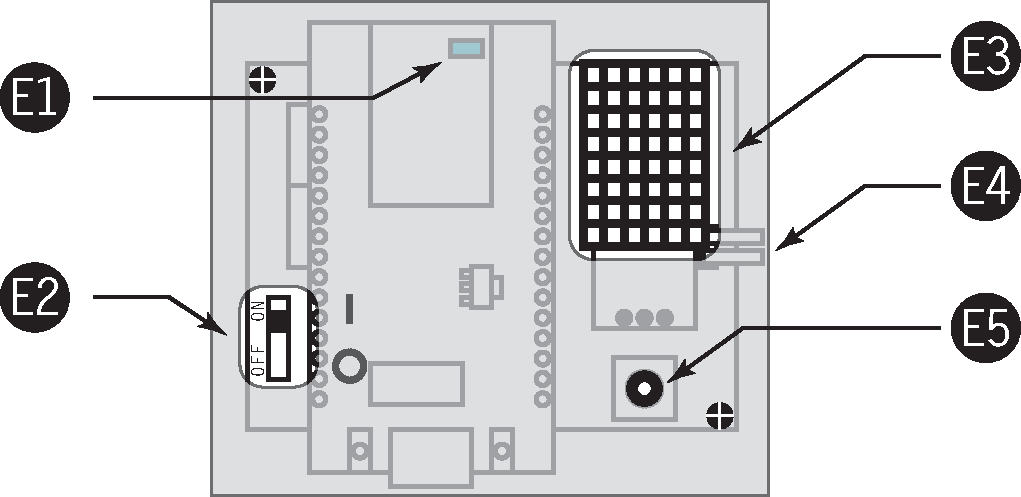
\includegraphics[width=0.8\columnwidth]{../design/exterior-controls}
  \caption{Controles del módulo exterior}
  \label{fig:exterior-controls}
\end{figure}
\section{Guía de inicio rápido}
\label{sec:inicio-rapido}

El \CMS requiere una configuración inicial para poder emplearse por primera vez.
Como mínimo, es necesario que se establezca el nombre y la contraseña de la red wifi a la que los módulos se conectarán para que puedan comunicarse.
Esta configuración debe realizarse tanto en el \MIE como en el \MEE.

\subsection{Configuración rápida del módulo interior}

El \MIE debe configurarse primero siguiendo los siguiente pasos:

\begin{enumeratecompact}

\item Mientras pulsa el botón multifunción \circled{I8}, conecte la alimentación USB \circled{I6} del \MI. Cuando la luz de notificación de configuración \circled{I3} se encienda de forma fija y en la pantalla LCD \circled{I1} aparezca el texto \emph{Conecta a Config.~Interior} (ver figura~\ref{fig:screen-config}, página \pageref{fig:screen-config}), suelte el botón \circled{I8}.

Si el mensaje \emph{Conecta a Config.~Interior} no aparece en la pantalla LCD, desconecte la alimentación y comience de nuevo. Alternativamente, en lugar de desconectar y conectar la alimentación USB \circled{I6}, puede presionar el botón de reinicio \circled{I5} mientras pulsa el botón multifunción \circled{I8}.

\item Con la ayuda de un dispositivo móvil o un ordenador con conexión wifi, busque las redes wifi disponibles y conecte a la red llamada \emph{Config.~Interior} (figura~\ref{fig:interior-select-wifi}, página~\pageref{fig:interior-select-wifi}).

\item En caso de que su dispositivo no le rediriga automáticamente a la página de configuración del \MI, despliegue el área de notificaciones de su dispositivo, y pulse la opción \emph{Iniciar sesión en red Wi-Fi ``Config.~Interior''} (figura~\ref{fig:interior-captive-portal-notification}, pá\-gi\-na~\pageref{fig:interior-captive-portal-notification}).

\item Seleccione la opción \emph{Configurar} (figura~\ref{fig:interior-menu}, página~\pageref{fig:interior-menu}).

\item Tras unos segundos, se mostrarán la lista de redes wifi detectadas por el \MI. Pulsando sobre el numbre de una red, se rellenará el campo \emph{SSID} (ver figura~\ref{fig:interior-config}). A continuación, escriba la contraseña de la red wifi seleccionada en el campo \emph{password}. Aplique los cambios pulsando el botón \emph{Guardar} al final de la página de configuración.

\item Se mostrará el mensaje \emph{Configuración guardada. Conectando a la red\ldots} El módulo se reiniciará en unos segundos. El \MI intentará conectarse automáticamente a la red configurada (ver figura~\ref{fig:screen-conn-process}, página~\pageref{fig:screen-conn-process}) y se quedará a la espera de que el \MEE esté listo (la luz de notificación de configuración \circled{I3} parpadeará). En caso de error (figura~\ref{fig:screen-conn-failed}, página~\pageref{fig:screen-conn-failed}), pruebe de nuevo desde el paso 1.

\end{enumeratecompact}


\subsection{Configuración rápida del módulo exterior}

El \MEE se debe configurar en segundo lugar siguiendo los pasos a continuación. El proceso de configuración del \MEE es similar al del \MIE:

\begin{enumeratecompact}

\item Asegúrese de que el \ME está apagado (interruptor de encendido \circled{E2} en posición \off).

\item Mientras pulsa el botón de configuración \circled{E5} con ayuda de alguna herramienta de punta estrecha y alargada, conecte el \ME moviendo el interruptor de encendido \circled{E2} a la posición \on. La luz de notificación de actividad \circled{E1} se encenderá momentáneamente. 

\item Con la ayuda de un dispositivo móvil o un ordenador con conexión wifi, busque las redes wifi disponibles y conecte a la red llamada \emph{Config.~Exterior} (figura~\ref{fig:exterior-select-wifi}).

\item En caso de que su dispositivo no le rediriga automáticamente a la página de configuración del \ME, despliegue el área de notificaciones de su dispositivo y pulse la opción \emph{Iniciar sesión en red Wi-Fi ``Config.~Exterior''} (figura~\ref{fig:exterior-captive-portal-notification}).

\item Seleccione la opción \emph{Configurar} (ver figura~\ref{fig:exterior-menu}).

\item Tras unos segundos, se mostrarán las redes wifi detectadas por el \ME. Pulsando sobre el numbre de una red, se rellenará el campo \emph{SSID} (ver figura~\ref{fig:exterior-config}). A continuación, escriba la contraseña de la red wifi seleccionada en el campo \emph{password}. Aplique los cambios pulsando el botón \emph{Guardar} al final de la página de configuración.

\item Se mostrará el mensaje \emph{Configuración guardada. Conectando a la red\ldots} El sistema se reiniciará en unos segundos. El \ME se conectará automáticamente a la red configurada y se sincronizará con el \MIE: la luz de notificación de configuración \circled{I3} dejará de papadear y se apagará, y en su lugar, se encenderá la luz de notificación de conexión \circled{I4}. Este proceso puede tardar hasta 45 segundos. En caso de error, pruebe de nuevo desde el paso 1.

\end{enumeratecompact}



\tipbegin{Configuración avanzada}
El \CMS permite configurar diversos parámetros de funcionamiento. Revise la sección~\ref{sec:gestion-avanzada} para ver opciones de gestión y configuración avanzadas.
\tipend



\section{Funcionamiento}
\label{sec:funcionamiento}

\begin{table}[!b]
\renewcommand\tabularxcolumn[1]{m{#1}}
\caption{Código de luces del \textit{Chana Monitoring System}}
\label{tab:luces}
\begin{tabularx}{\textwidth}{ccX}
\toprule
\headingc{Color} & \headingc{Estado} & \headingc{Descripción} \\
\topruleb
  \circlefilled{red}    & \textsc{\textbf{apagado}}      & Sin errores. Comprobar \circlefilled{yellow} y \circlefilled{green} para más datos.\\*\midrule
  \circlefilled{red}    & \textsc{\textbf{fijo}}         & El \MIE ha perdido conexión con el \MEE durante demasiado tiempo.\\*\midrule
  \circlefilled{red}    & \textsc{\textbf{intermitente}} & El \MEE ha detectado que el depósito está lleno.\\*\midrule
  \circlefilled{yellow} & \textsc{\textbf{apagado}}      & El \MIE se inició correctamente y se sincronizó con el \ME. Comprobar \circlefilled{red} y \circlefilled{green} para más datos.\\*\midrule
  \circlefilled{yellow} & \textsc{\textbf{fijo}}         & El \MIE está intentando conectar a una red wifi o está en modo gestión.\\*\midrule
  \circlefilled{yellow} & \textsc{\textbf{intermitente}} & El \MIE se ha iniciado correctamente, pero no se ha sincronizado con el \MEE aún.\\*\midrule
  \circlefilled{green}  & \textsc{\textbf{apagado}}      & No hay/ha habido conexión entre el \MIE y el \MEE. Comprobar \circlefilled{red} y \circlefilled{yellow} para más datos.\\*\midrule
  \circlefilled{green}  & \textsc{\textbf{fijo}}         & El \CMS funciona normalmente.\\*\midrule
  \circlefilled{green}  & \textsc{\textbf{intermitente}} & El \CMS funciona normalmente, pero el \MEE tiene la batería baja.\\*\bottomrule
\end{tabularx}
\end{table}

Con el objetivo de maximizar el tiempo de vida de las batería del \MEE, el \MIE es quien proporciona toda la información al usuario del \CMS a través de alarmas sonoras, los testigos \circled{I2}, \circled{I3} e \circled{I4} y la pantalla LCD \circled{I1}. Los testigos y las alarmas sonoras permiten comprobar el estado del \CMS de un vistazo rápido, sin necesidad de comprobar los mensajes que se muestran en la pantalla LCD \circled{I1}. La tabla~\ref{tab:luces} resume los principales estados que representan los diferentes testigos de colores.



En las siguientes subsecciones, se describne en detalle las diferentes informaciones que puede mostrar el \CMS.

\subsection{Arranque}

Cuando el \MIE se conecta a la alimentación USB, éste se enciende de forma automática e intenta conectarse a la red wifi que haya sido configurada a través de la interfaz de gestión (ver sección~\ref{sec:gestion-avanzada}, \textit{\nameref{sec:gestion-avanzada}}). Esto se notifica mediante el testigo de configuración \circled{I3} encendido de forma fija (\circlefilled{yellow}), y mostrando el mensaje \emph{Conectando a red WiFi\ldots} en la pantalla LCD \circled{I1} tal y como muestra la figura \ref{fig:screen-conn-process}.

\begin{figure}[!b]
  \centering
  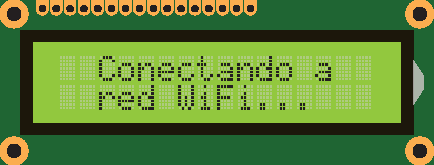
\includegraphics[width=0.6\columnwidth]{images/screen-conn-process}
  \caption{Pantalla del módulo interior -- Conectando a red wifi}
  \label{fig:screen-conn-process}
\end{figure}

\begin{figure}[!b]
  \centering
  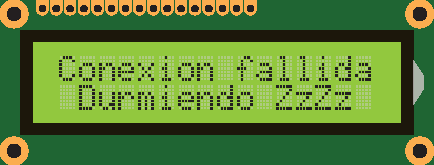
\includegraphics[width=0.6\columnwidth]{images/screen-conn-failed}
  \caption{Pantalla del módulo interior -- fallo de conexión}
  \label{fig:screen-conn-failed}
\end{figure}


En caso de que la conexión falle, el sistema apagará todos los testigos y mostrará el mensaje \emph{Conexion fallida / Durmiendo ZzZz} tal y como muestra la figura~\ref{fig:screen-conn-failed}. El \MI se quedará en ese estado de hibernación hasta que el usuario lo reinicie y compruebe por qué no ha sido posible realizar la conexión (error puntual, cobertura wifi deficiente, \etc).



\subsection{El menú de información}
\label{sec:menu-info}

El menú de información se muestra cuando el \MIE ha arrancado y se ha conectado a una red wifi de forma satisfactoria. Consta de 5 pantallas, que pueden navegarse en la secuencia
~~~\tikz[baseline=-0.63ex,node distance=1em,remember picture]{
\node (n1) {1};
\node (n2) [right=of n1] {2};
\node (n3) [right=of n2] {3};
\node (n4) [right=of n3] {4};
\node (n5) [right=of n4] {5};
\draw[->] (n1) -> (n2);
\draw[->] (n2) -> (n3);
\draw[->] (n3) -> (n4);
\draw[->] (n4) -> (n5);
}
\tikz[remember picture,overlay]{
\draw[->,smooth]  (n5)
to[out=0, in=180]  ($(n5) + ( 0.3cm, 0.00cm)$)
to[out=0, in=0]    ($(n5) + ( 0.3cm,-0.22cm)$)
to[out=180,in=0]   ($(n1) + (-0.3cm,-0.22cm)$)
to[out=180,in=180] ($(n1) + (-0.3cm, 0.00cm)$)
to[out=0, in=180] (n1);
}~~
pulsando el botón multifunción~\circled{I8}.

\textbf{Pasados 60 segundos desde la última pulsación del botón multifunción \circled{I8}, el \MI volverá automáticamente a la pantalla 1.}

\attbegin{Pantallas 1 y 2}
Nada más iniciarse, y mientras el testigo de configuración \circled{I3} se enciende de forma \textbf{intermitente} (\circlefilled{yellow}), sólo se mostrarán las pantallas 3 a 5 hasta que el \MEE realice la primera sincronización de datos y se encienda el testigo de conexión \circled{I4} (\circlefilled{green}).

\textbf{En ese caso, al pasar 60 segundos sin pulsar el botón multifunción \circled{I8}, el \MI volverá automáticamente a la pantalla 3 en lugar de a la pantalla~1.}
\attend

Las pantallas de información que muestre el \MIE en su modo de operación normal son:

\begin{descriptioncompact}

\begin{figure}[!b]
  \centering
  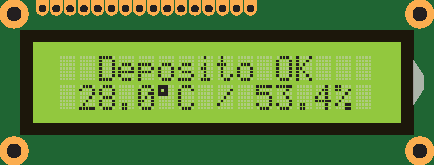
\includegraphics[width=0.6\columnwidth]{images/screen1}
  \caption{Pantalla 1 del módulo interior -- Información exterior}
  \label{fig:screen1}
\end{figure}

\item[Pantalla 1: Información exterior] --- Esta pantalla sólo se muestra cuando el \MEE ha enviado datos de estado recientemente. Como muestra la figura~\ref{fig:screen1}, la primera línea muestra el estado del depósito, mientras que la segunda línea muestra la temperatura y porcentaje de humedad exteriores.

\begin{figure}[t]
\centering
\begin{subfigure}{0.6\columnwidth}
  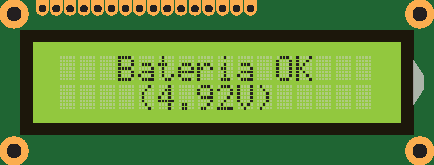
\includegraphics[width=1\columnwidth]{images/screen2a}
  \caption{}
  \label{fig:screen2a}
\end{subfigure}
\\[1em]
\begin{subfigure}{0.6\columnwidth}
  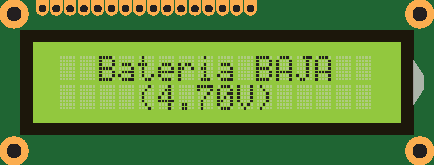
\includegraphics[width=1\columnwidth]{images/screen2b}
  \caption{}
  \label{fig:screen2b}
\end{subfigure}
\caption{Pantalla 2 del módulo interior -- información de batería}
\label{fig:screen2}
\end{figure}

\item[Pantalla 2: información de batería] --- Al igual que la pantalla 1, esta pantalla sólo se muestra cuando el \MEE ha enviado datos de estado recientemente. Como muestra la figura~\ref{fig:screen2}, la primera línea muestra el estado de la batería según el \emph{Umbral de batería baja} (ver sección~\ref{sec:params-interior}, \textit{\nameref{sec:params-interior}}), mientras que la segunda línea muestra el detalle de la tensión proporcionada por las baterías del \MEE. Cuando se muestra el mensaje de \emph{Bateria BAJA}, el testigo de conexión \circled{I4} (\circlefilled{green}) estará encendida de forma intermitente.

\attbegin{Umbral de batería baja}
La temperatura exterior puede afectar al nivel de batería detectado en \mbox{$\pm$0,1 V}. Por tanto, es normal que existan variaciones mínimas en el nivel de batería a lo largo del día. Igualmente, cuando el nivel de batería esté cerca del umbral de batería baja, es normal que el \MIE cambie frecuentemente entre \emph{Batería OK} y \emph{Bateria BAJA} dependiendo de las variaciones de la temperatura exterior.
\attend

\begin{figure}
  \centering
  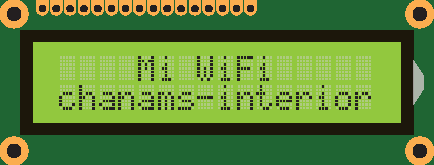
\includegraphics[width=0.6\columnwidth]{images/screen3}
  \caption{Pantalla 3 del módulo interior -- información de red}
  \label{fig:screen3}
\end{figure}


\item[Pantalla 3: información de red] --- Ésta es la primera pantalla que se muestra cuan\-do el \MIE acaba de iniciarse, el \MEE todavía no ha enviado datos, y el testigo de configuración \circled{I3} (\circlefilled{yellow}) todavía se enciende de forma intermitente. Como muestra la figura~\ref{fig:screen3}, en la primera línea se muestra el nombre de la red wifi a la que se encuentre conectado el \ME (hasta un máximo de 16 caracteres), mientras que la segunda línea muestra el \emph{Nombre de host} que se ha especificado en la configuración del \MI (ver sección~\ref{sec:params-interior}). Aquellos dispositivos que soportan el protocolo \emph{mDNS} pueden conectarse al \MI empleando el nombre de host que aquí aparece añadiendo el sufijo \texttt{.local} (por ejemplo, \texttt{chanams-interior.local}). 

\item[Pantalla 4: IP y puerto de escucha] --- Esta pantalla muestra más información de red. La primera línea muestra la dirección IP del \MIE~---útil cuando se desea conectar al \MI un dispositivo que no soporta el protocolo mDNS--- mientras que la segunda muestra el \emph{Puerto de escucha} (ver sección~\ref{sec:params-interior}).

\begin{figure}
  \centering
  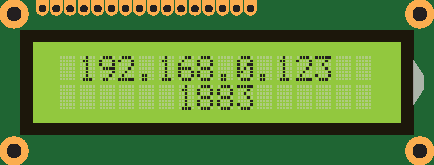
\includegraphics[width=0.6\columnwidth]{images/screen4}
  \caption{Pantalla 4 del módulo interior -- IP y puerto de escucha}
  \label{fig:screen4}
\end{figure}

\begin{figure}
  \centering
  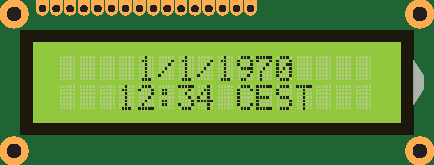
\includegraphics[width=0.6\columnwidth]{images/screen5}
  \caption{Pantalla 5 del módulo interior -- fecha y hora}
  \label{fig:screen5}
\end{figure}

\item[Pantalla 5: fecha y hora] --- Esta pantalla muestra la fecha y hora según la zona horaria que se ha establecido en las opciones de configuración (de nuevo, ver sección~\ref{sec:params-interior}). Dadas las características del hardware del \CMS (que no dispone de reloj interno), la fecha y la hora se obtienen de internet. La primera línea muestra la fecha, mientras que la segunda muestra la hora y la zona horaria, por ejemplo, CEST (\textit{Central European Summer Time} u hora de verano de Europa central), CET (\textit{Central European Time} u hora de invierno de Europa central),~\etc

\end{descriptioncompact}


\subsection{Avisos y alarmas sonoras}
\label{sec:alarmas}

Además de los testigos luminosos, el \CMS puede lanzar avisos y alarmas sonoras para alertar de los eventos críticos que requiren de una acción in\-me\-diata del usuario.

\tipbegin{Modo silencio permanente}
Es posible desactivar todas las alarmas sonoras de forma permanente colocando el interruptor de la alarma sonora \circled{I8} en la posición \off.
\tipend

\tipbegin{Silencio automático}
Además del modo de silencio permanente, el \CMS puede silenciarse automáticamente durante una determinada franja horaria, por ejemplo, para evitar avisos sonoros durante la noche. Vea la sección~\ref{sec:params-interior} (\textit{\nameref{sec:params-interior}}) para más información.
\tipend

\tipbegin{Comprobación de estado de las alarmas sonoras}
En caso de duda, es posible comprobar si el \CMS se encuentra en modo de silencio permanente pulsando el botón de reinicio \circled{I5} ---o desconectando momentáneamente la alimentación USB \circled{I6}--- del \MIE. Si el modo de silencio permanente está \textbf{activado}, el \CMS no emitirá ningún sonido. Si el modo de silencio permanente está \textbf{desactivado}, el \CMS emitirá tres pitidos cortos al iniciarse. \textbf{Los tres pitidos se emitirán incluso en el periodo de silencio automático.}
\tipend


Los avisos y alarmas que emite el \CMS son:

\begin{descriptioncompact}

\item[Aviso de batería baja] --- Cuando la tensión proporcionada por la batería del \MEE está por debajo del umbral configurado (véase \emph{Umbral de batería baja} en la sección~\ref{sec:params-interior}), el \MIE lo notifica regularmente emitiendo un breve pitido agudo en todas las horas en punto ---o en la primera sincronización cuando el \CMS acaba de conectarse--- hasta que las baterías son reemplazadas.

Recuerde que cuando el \ME notifica un valor por debajo del \emph{Umbral de batería baja}, el testigo de conexión \circled{I4} (\circlefilled{green}) permanece encendido de forma intermitente.


\item[Alarma de depósito lleno] --- Cuando el \MEE notifica que el depósito se ha llenado, el \MIE emite breves pitidos graves de forma continua durante 60 segundos (o hasta que se pulsa el botón multifución \circled{I8}).
La secuencia de pitidos de 60 segundos de duración se repite cada varios minutos (según el \emph{Tiempo de espera entre mensajes}, véase la sección~\ref{sec:params-exterior}) mientras el depósito permanece lleno.

Cuando el aviso de depósito lleno se dispara, el menú de información del \MIE se bloquea, la pantalla LCD \circled{I1} muestra el mensaje \emph{!!! ALERTA !!! / DEPO\-SITO LLENO} (ver figura~\ref{fig:screen-deposit-full}), y el testigo de fallo \circled{I2} (\circlefilled{red}) permanece encendido de forma intermitente hasta que se vacía el depósito. 

\begin{figure}
  \centering
  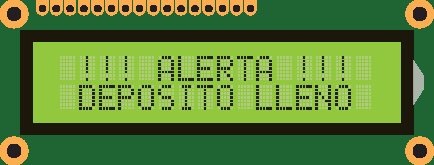
\includegraphics[width=0.6\columnwidth]{images/screen-deposit-full}
  \caption{Pantalla del módulo interior: depósito lleno}
  \label{fig:screen-deposit-full}
\end{figure}

\begin{figure}
  \centering
  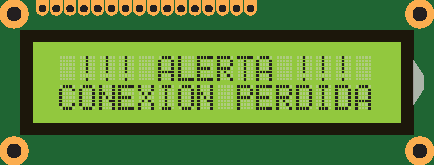
\includegraphics[width=0.6\columnwidth]{images/screen-conn-lost}
  \caption{Pantalla del módulo interior: conexión perdida}
  \label{fig:screen-conn-lost}
\end{figure}

\item[Alarma de conexión perdida] --- Cuando el \MIE no recibe ninguna información por parte del \MEE durante demasiado tiempo (véase \emph{Tiempo de espera máximo} en la sección~\ref{sec:params-interior}, \textit{\nameref{sec:params-interior}}), el \MIE emite un pitido agudo y un pitido grave ---emulando una sirena--- de forma continua hasta que la conexión con el \MEE se restaura o la alarma se silencia pulsando el botón multifunción \circled{I8}.   

Cuando el aviso de conexión perdida se dispara, el menú de información del \MIE se bloquea, la pantalla LCD \circled{I1} muestra el mensaje \emph{!!! ALERTA !!! / CONEXION PERDIDA} (véase figura~\ref{fig:screen-conn-lost}), y el testigo de fallo \circled{I2} (\circlefilled{red}) permanece encendido de forma fija hasta que se restaura la conexión entre los módulos interior y exterior. 



\attbegin{En caso de conexión perdida}
En caso de conexión perdida, revise el procedimiento detallado en la sección~\ref{sec:conn-perdida} (\textit{\nameref{sec:conn-perdida}}).
\attend

\end{descriptioncompact}


\cleardoublepage


\section{Gestión avanzada}
\label{sec:gestion-avanzada}

El \CMS se gestiona a través de una interfaz web en modo de \emph{portal cautivo} que se activa cuando se accede al modo de gestión tanto del \MI como del \ME.
Ambos módulos proporcionan portales de gestión con la misma estructura y funcionalidad: la única diferencia entre ellos se encuentra en los parámetros de funcionamiento que se pueden configurar.

A continuación se detallan los pasos a seguir para acceder al modo de gestión, así como las diferentes funciones y opciones que se proporcionan.

\subsection{Acceso a la interfaz de gestión}
\label{sec:acceso-gestion}

Como se introduce en la sección~\ref{sec:inicio-rapido} (\textit{\nameref{sec:inicio-rapido}}), el modo de acceso a la interfaz de gestión es el mismo en ambos casos: presionar el único botón independiente que presentan los módulos a la vez se encienden o se reinician.

Para activar la interfaz de gestion del \MIE se hace uso del botón multifunción \circled{I8}:

\begin{enumeratecompact}

\item Mientras pulsa el botón multifunción \circled{I8}, conecte la alimentación USB \circled{I6} del \MI. Si la alimentación ya está conectada, alternativamente, puede presionar el botón de reinicio \circled{I5} mientras pulsa el botón multifunción \circled{I8}. Cuando el testigo de configuración \circled{I3} se encienda de forma fija y en la pantalla LCD \circled{I1} aparezca el texto \emph{Conecta a Config.~Interior} (figura~\ref{fig:screen-config}), suelte el botón \circled{I8}.

\begin{figure}[!b]
  \centering
  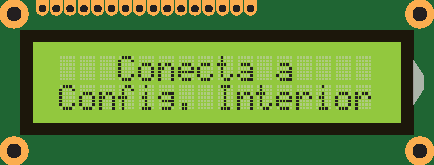
\includegraphics[width=0.6\columnwidth]{images/screen-config}
  \caption{Pantalla del módulo interior: modo gestión}
  \label{fig:screen-config}
\end{figure}

Si el mensaje \emph{Conecta a Config.~Interior} no aparece en la pantalla LCD, comience de nuevo.

\item Con la ayuda de un dispositivo móvil o un ordenador con conexión wifi, busque las redes wifi disponibles y conecte a la red llamada \emph{Config.~Interior} (figura~\ref{fig:interior-select-wifi}, página~\pageref{fig:interior-select-wifi}).

\item En caso de que su dispositivo no le rediriga automáticamente a la página de configuración del \MI, despliegue el área de notificaciones de su dispositivo y pulse la opción \emph{Iniciar sesión en red Wi-Fi ``Config.~Interior''} (figura~\ref{fig:interior-captive-portal-notification}, pá\-gi\-na~\pageref{fig:interior-captive-portal-notification}).

\item El menú mostrado en la figura~\ref{fig:interior-menu} aparecerá en su pantalla.

\end{enumeratecompact}

En el caso del \MEE, la activación de la interfaz de gestión se realiza mediante el botón de configuración \circled{E4}:

\begin{enumeratecompact}

\item Asegúrese de que el \ME está apagado (interruptor de encendido \circled{E2} en posición \off).

\item Mientras pulsa el botón de configuración \circled{E5} con ayuda de alguna herramienta de punta estrecha y alargada, conecte el \ME moviendo el interruptor de encendido \circled{E2} a la posición \on. El testigo de actividad \circled{E1} emitirá un breve destello. 

\item Con la ayuda de un dispositivo móvil o un ordenador con conexión wifi, busque las redes wifi disponibles y conecte a la red llamada \emph{Config.~Exterior} (figura~\ref{fig:exterior-select-wifi}).

\item En caso de que su dispositivo no le rediriga automáticamente a la página de configuración del \ME, despliegue el área de notificaciones de su dispositivo y pulse la opción \emph{Iniciar sesión en red Wi-Fi ``Config.~Exterior''} (figura~\ref{fig:exterior-captive-portal-notification}).

\item El menú mostrado en la figura~\ref{fig:exterior-menu} aparecerá en su pantalla.

\end{enumeratecompact}

\begin{figure}
\begin{subfigure}{0.49\columnwidth}
  \centering
  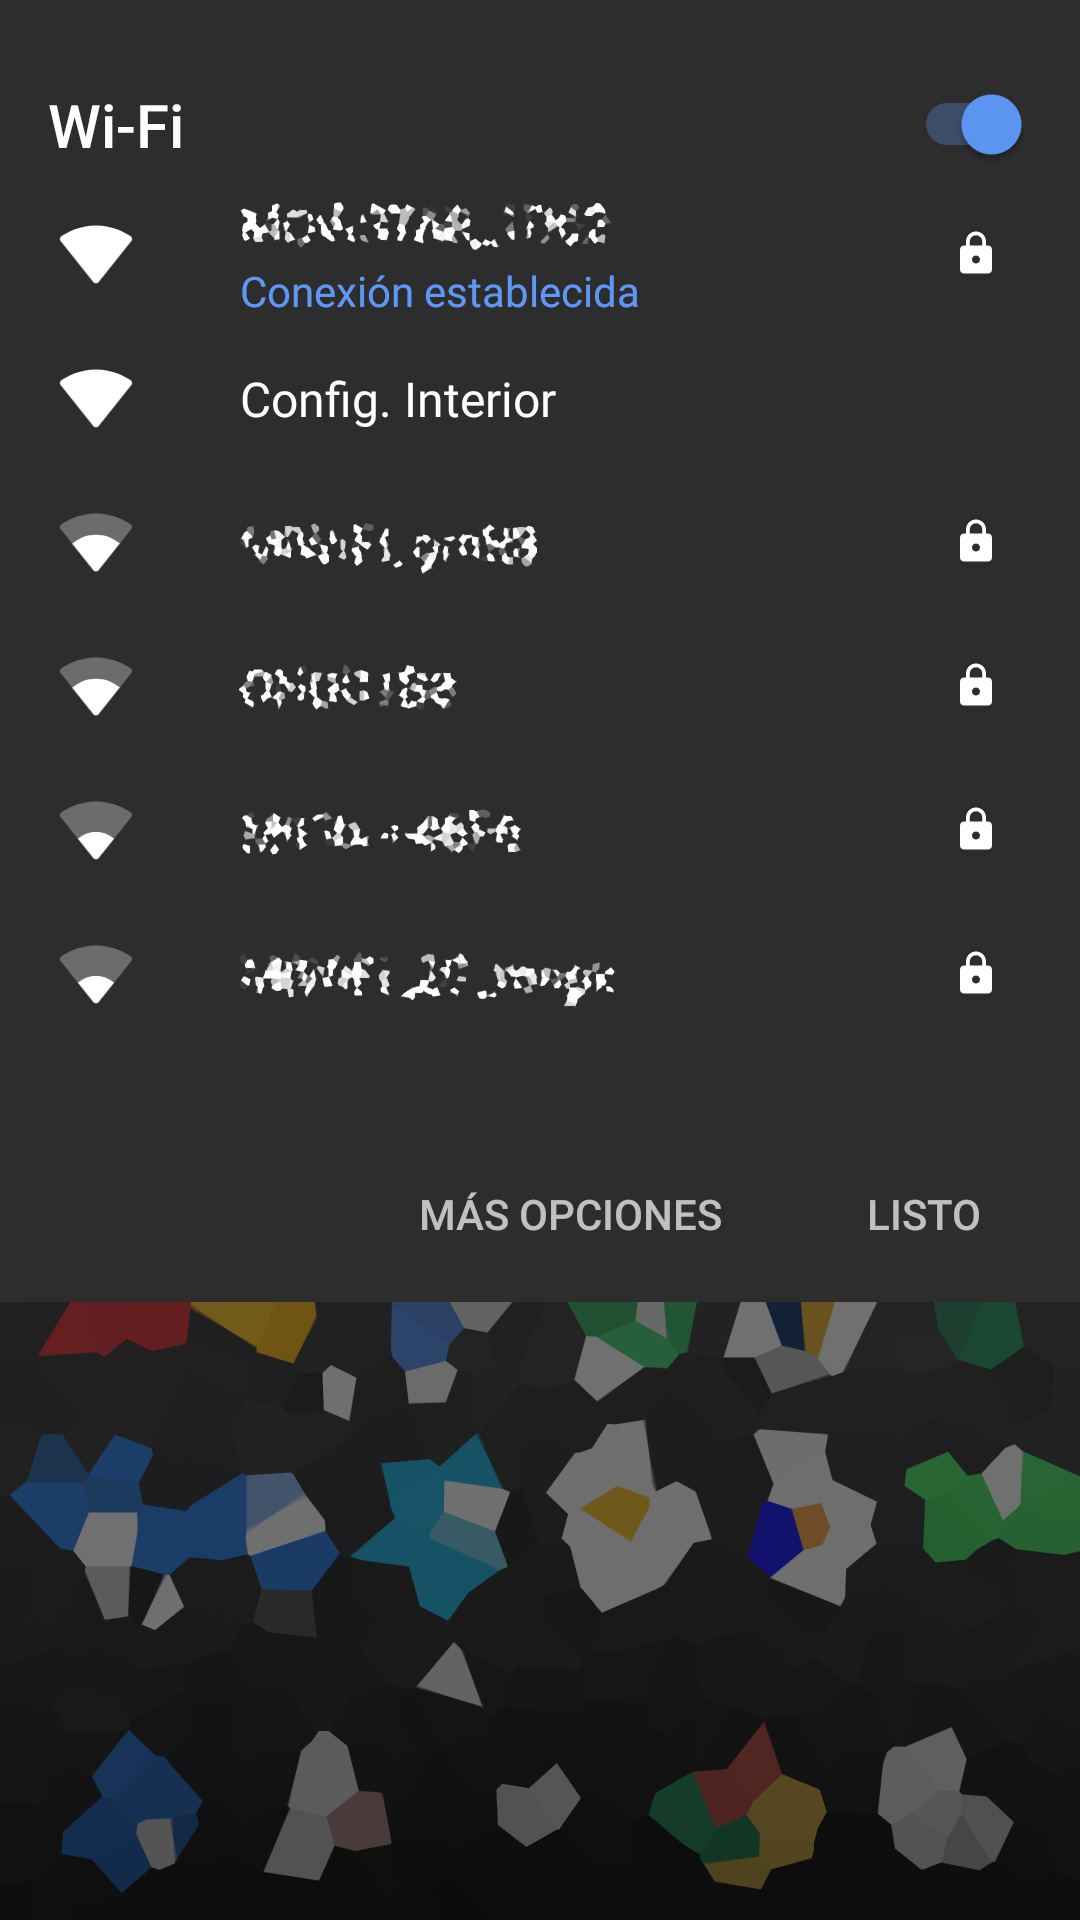
\includegraphics[width=1\columnwidth,frame]{images/interior-select-wifi}
  \caption{}
  \label{fig:interior-select-wifi}
\end{subfigure}
\hfill
\begin{subfigure}{0.49\columnwidth}
  \centering
  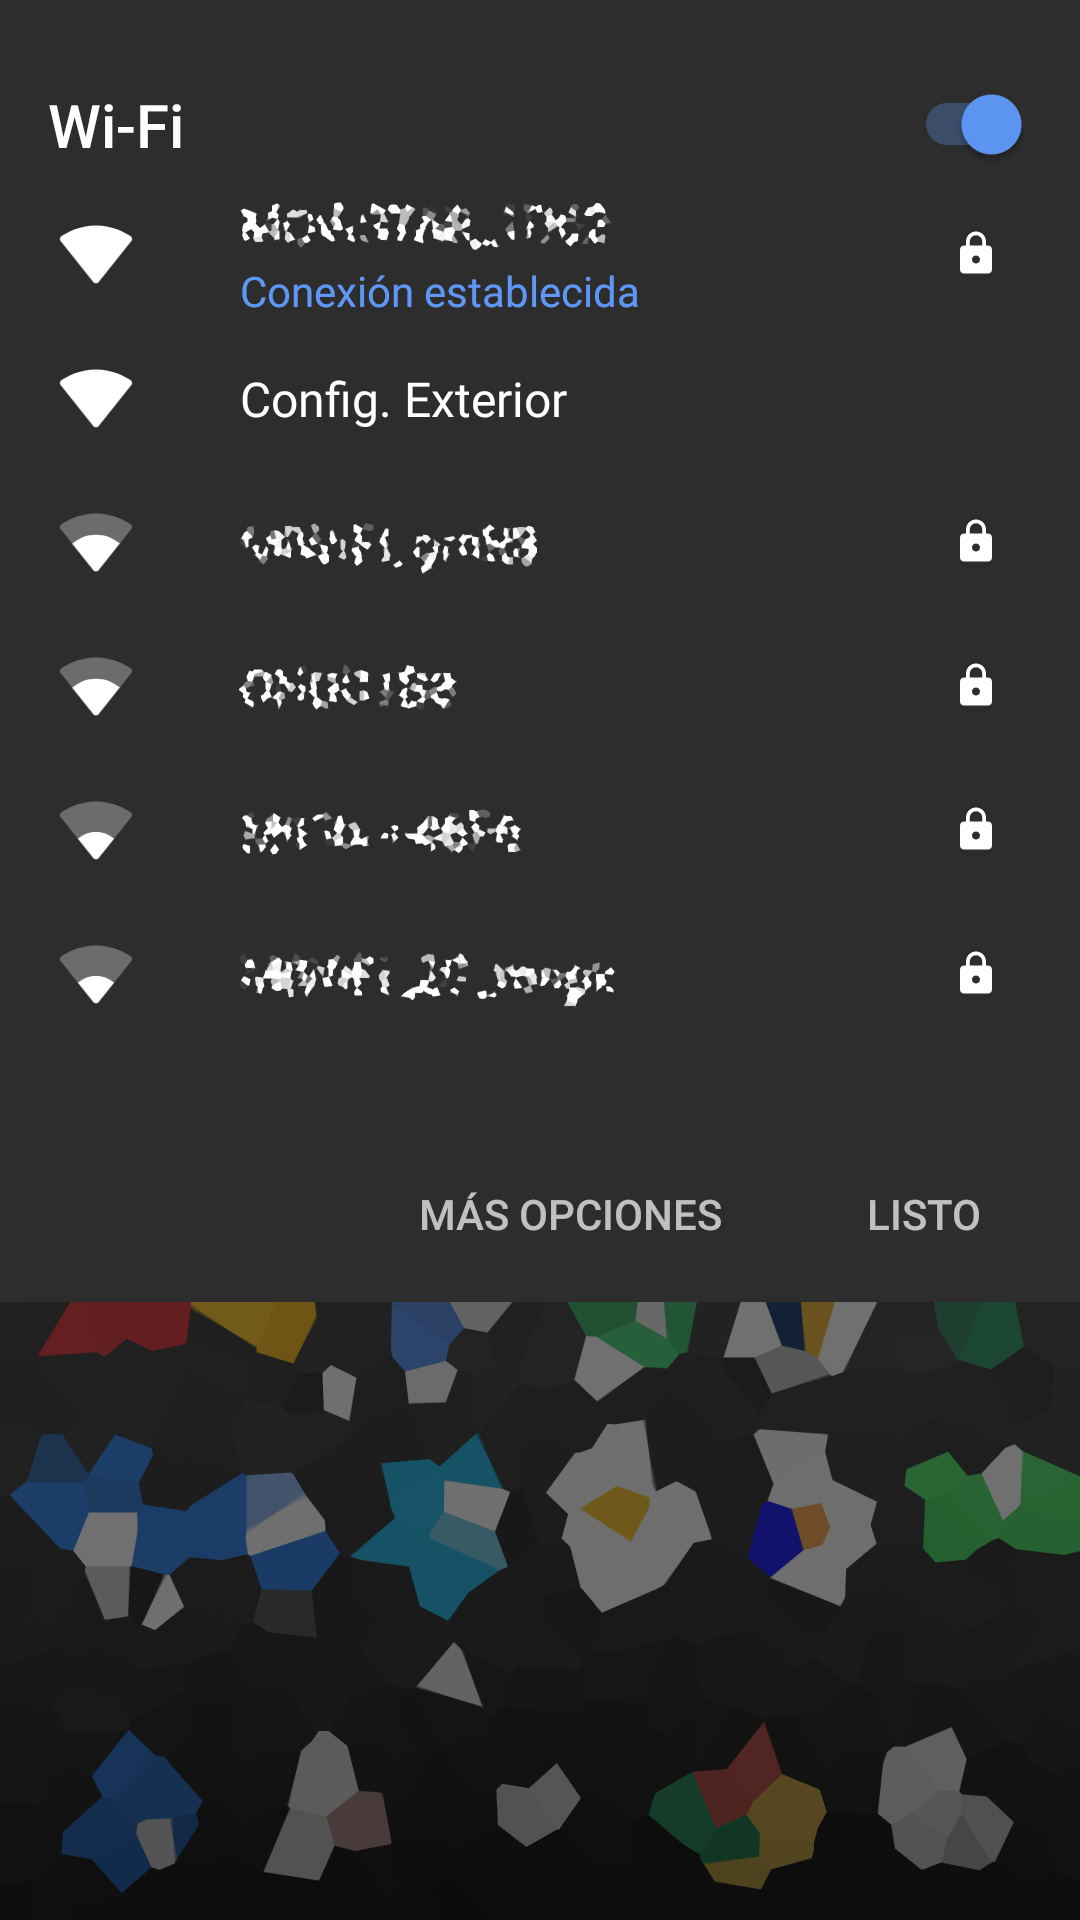
\includegraphics[width=1\columnwidth,frame]{images/exterior-select-wifi}
  \caption{}
  \label{fig:exterior-select-wifi}
\end{subfigure}
\caption{Conectar a las redes \textit{Config.~Interior} (a) y \textit{Config.~Exterior} (b)}
\end{figure}

\begin{figure}
\begin{subfigure}{0.49\columnwidth}
  \centering
  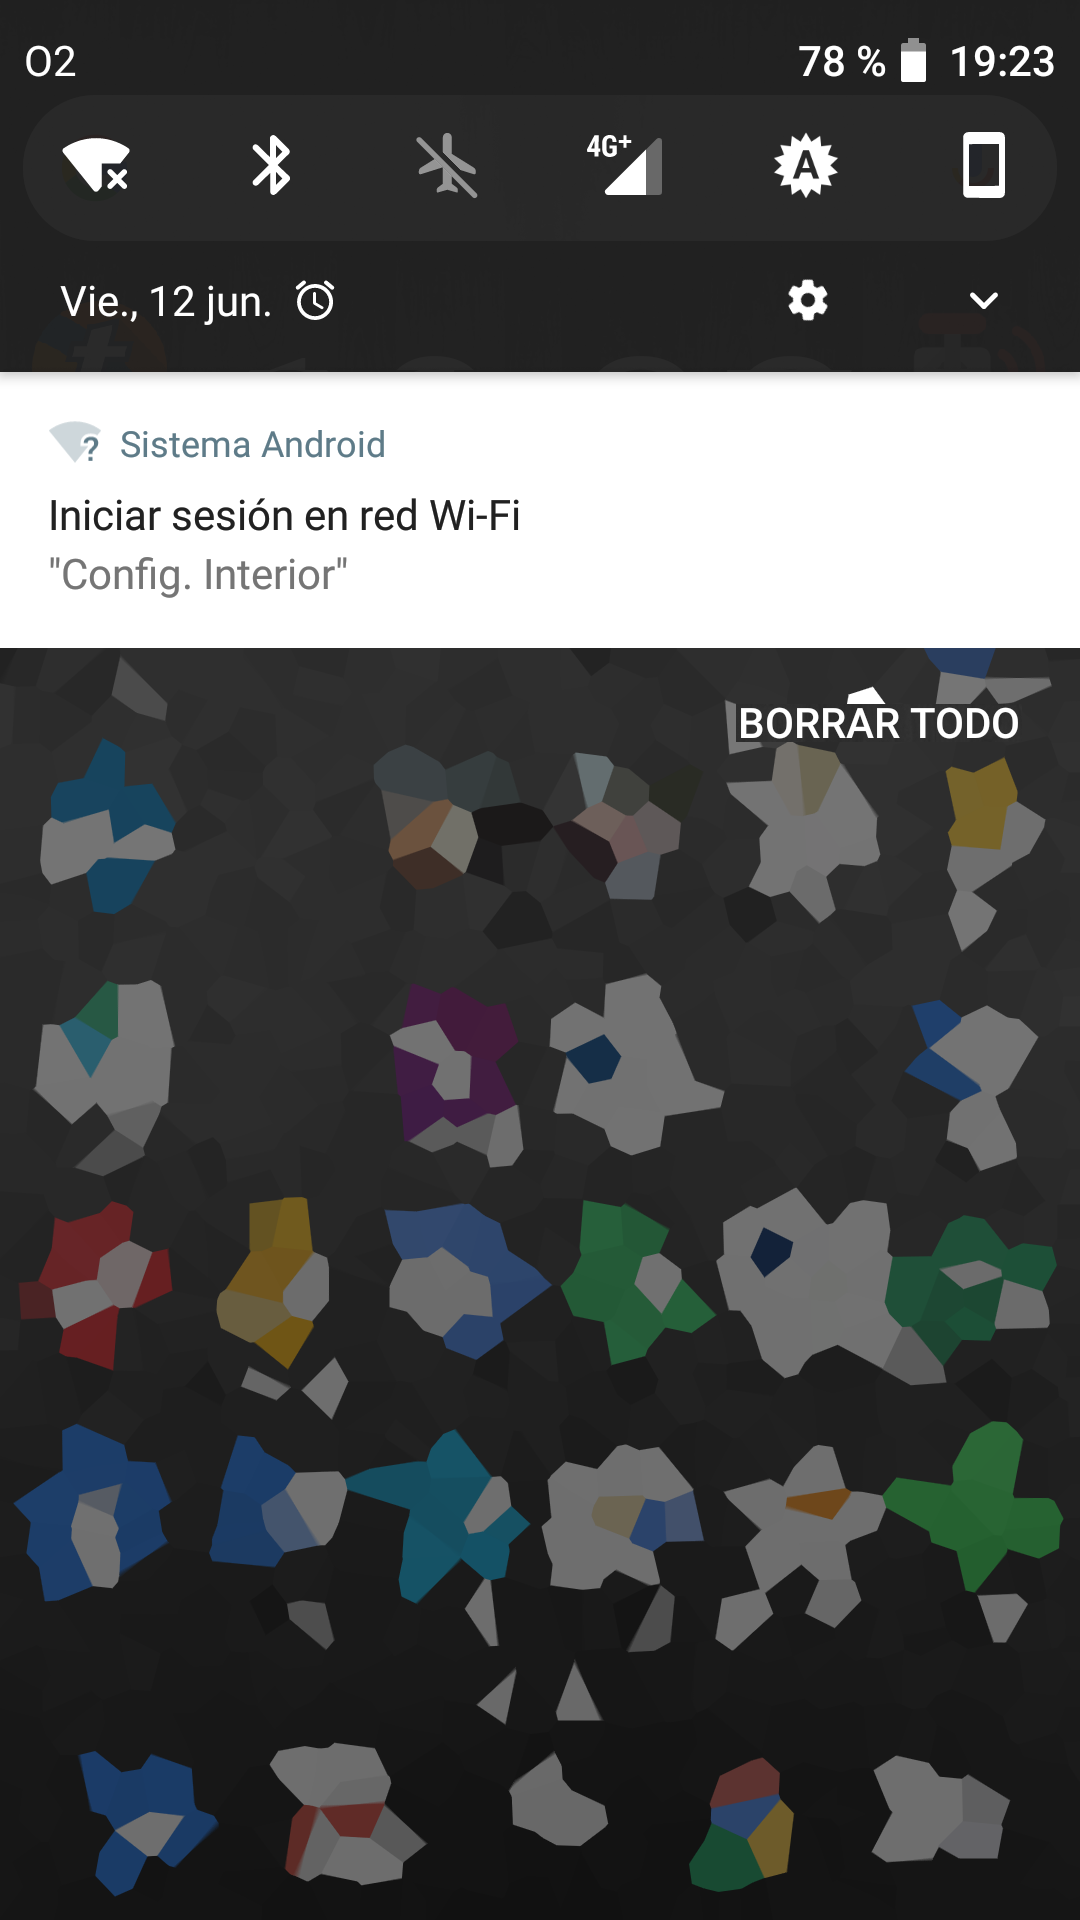
\includegraphics[width=1\columnwidth,frame]{images/interior-captive-portal-notification}
  \caption{}
  \label{fig:interior-captive-portal-notification}
\end{subfigure}
\hfill
\begin{subfigure}{0.49\columnwidth}
  \centering
  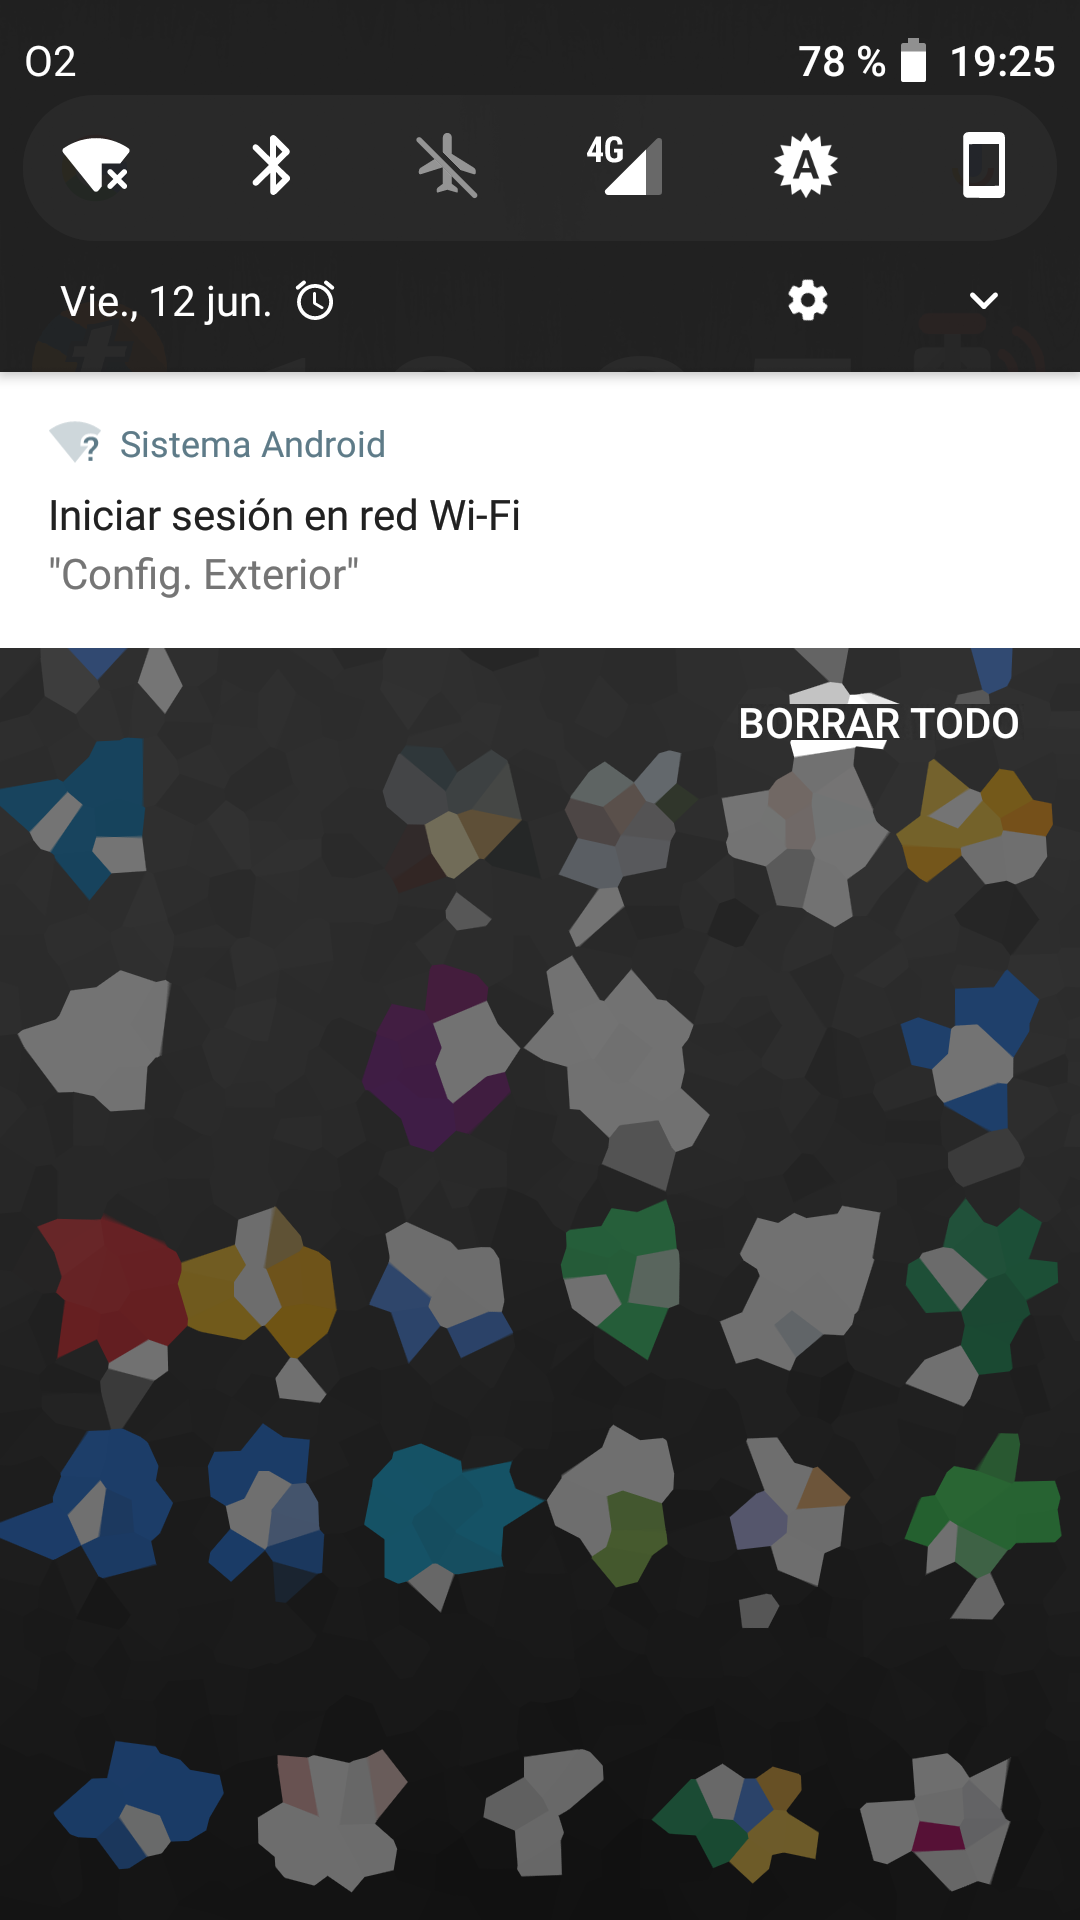
\includegraphics[width=1\columnwidth,frame]{images/exterior-captive-portal-notification}
  \caption{}
  \label{fig:exterior-captive-portal-notification}
\end{subfigure}
\caption{Iniciar sesión en las redes \textit{Config.~Interior} (a) y \textit{Config.~Exterior} (b)}
\end{figure}


\begin{figure}
\begin{subfigure}{0.49\columnwidth}
  \centering
  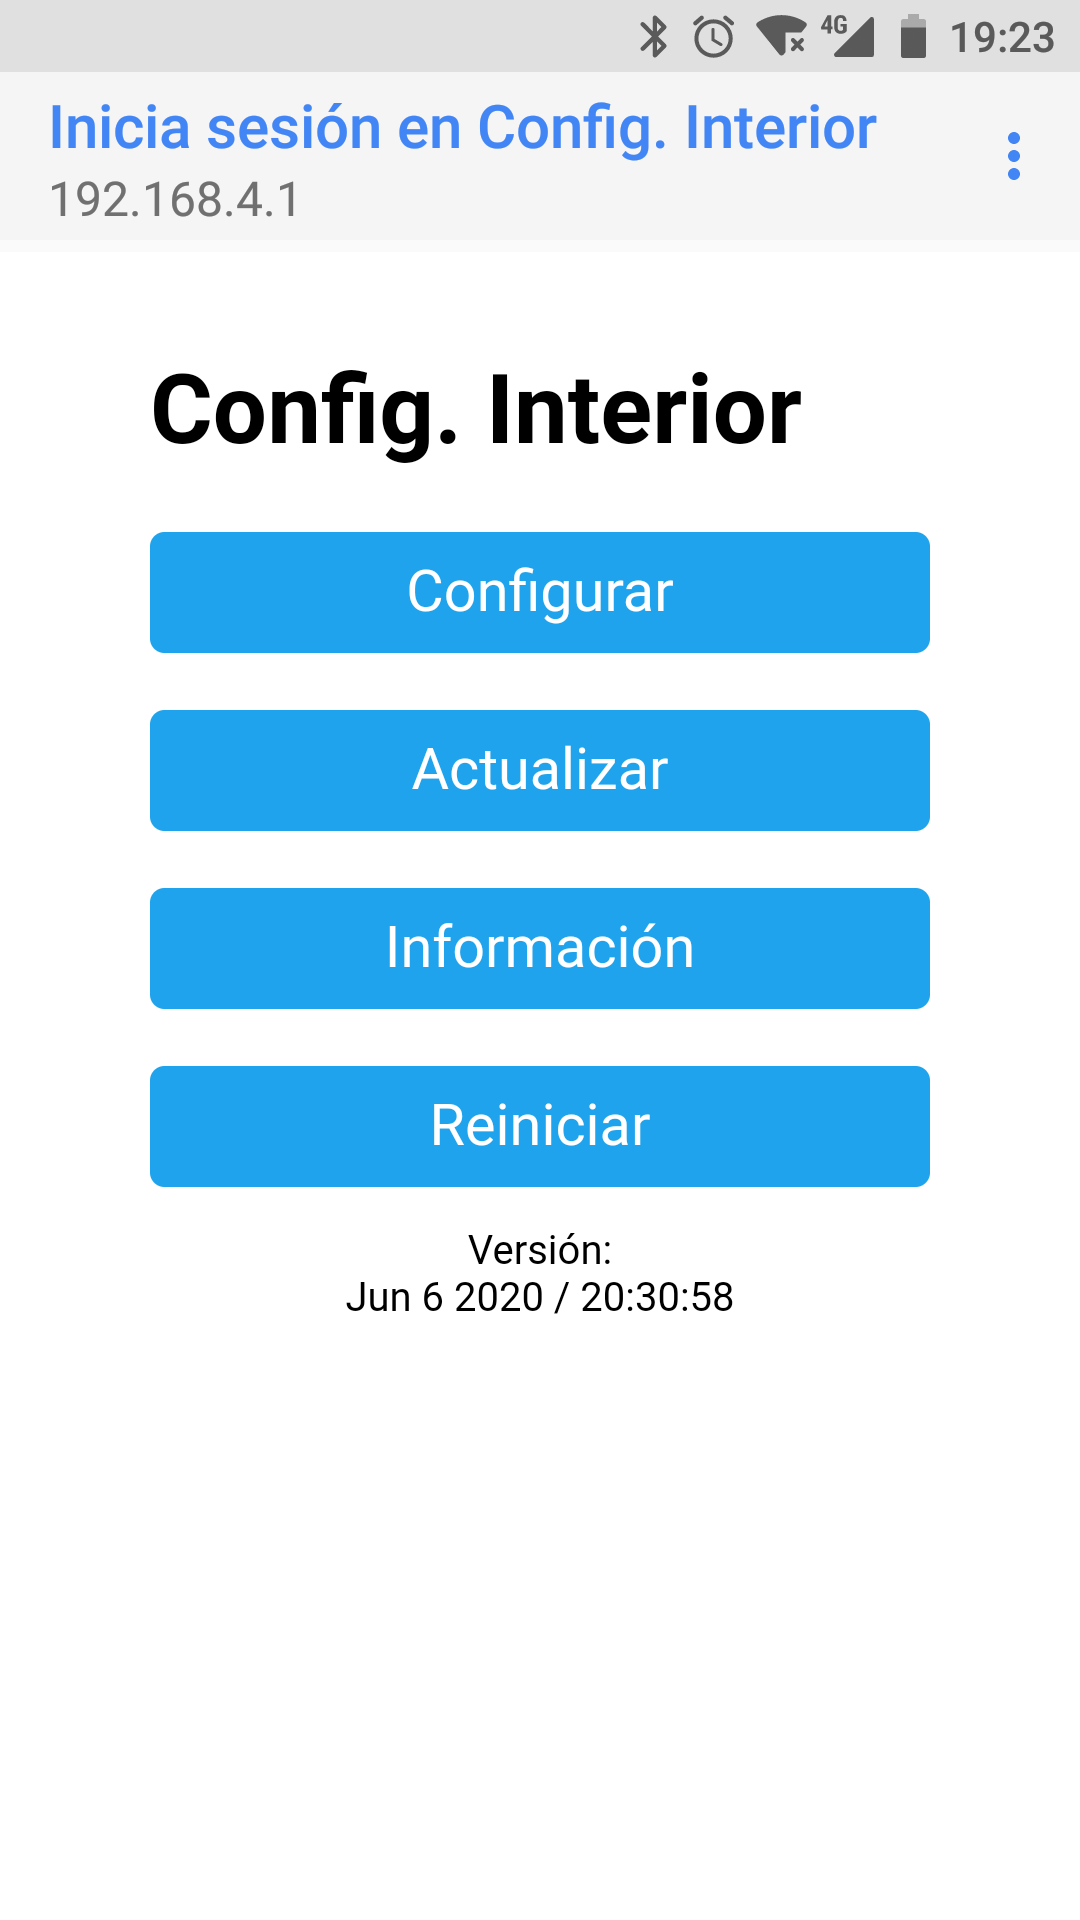
\includegraphics[width=1\columnwidth,frame]{images/interior-menu}
  \caption{}
  \label{fig:interior-menu}
\end{subfigure}
\hfill
\begin{subfigure}{0.49\columnwidth}
  \centering
  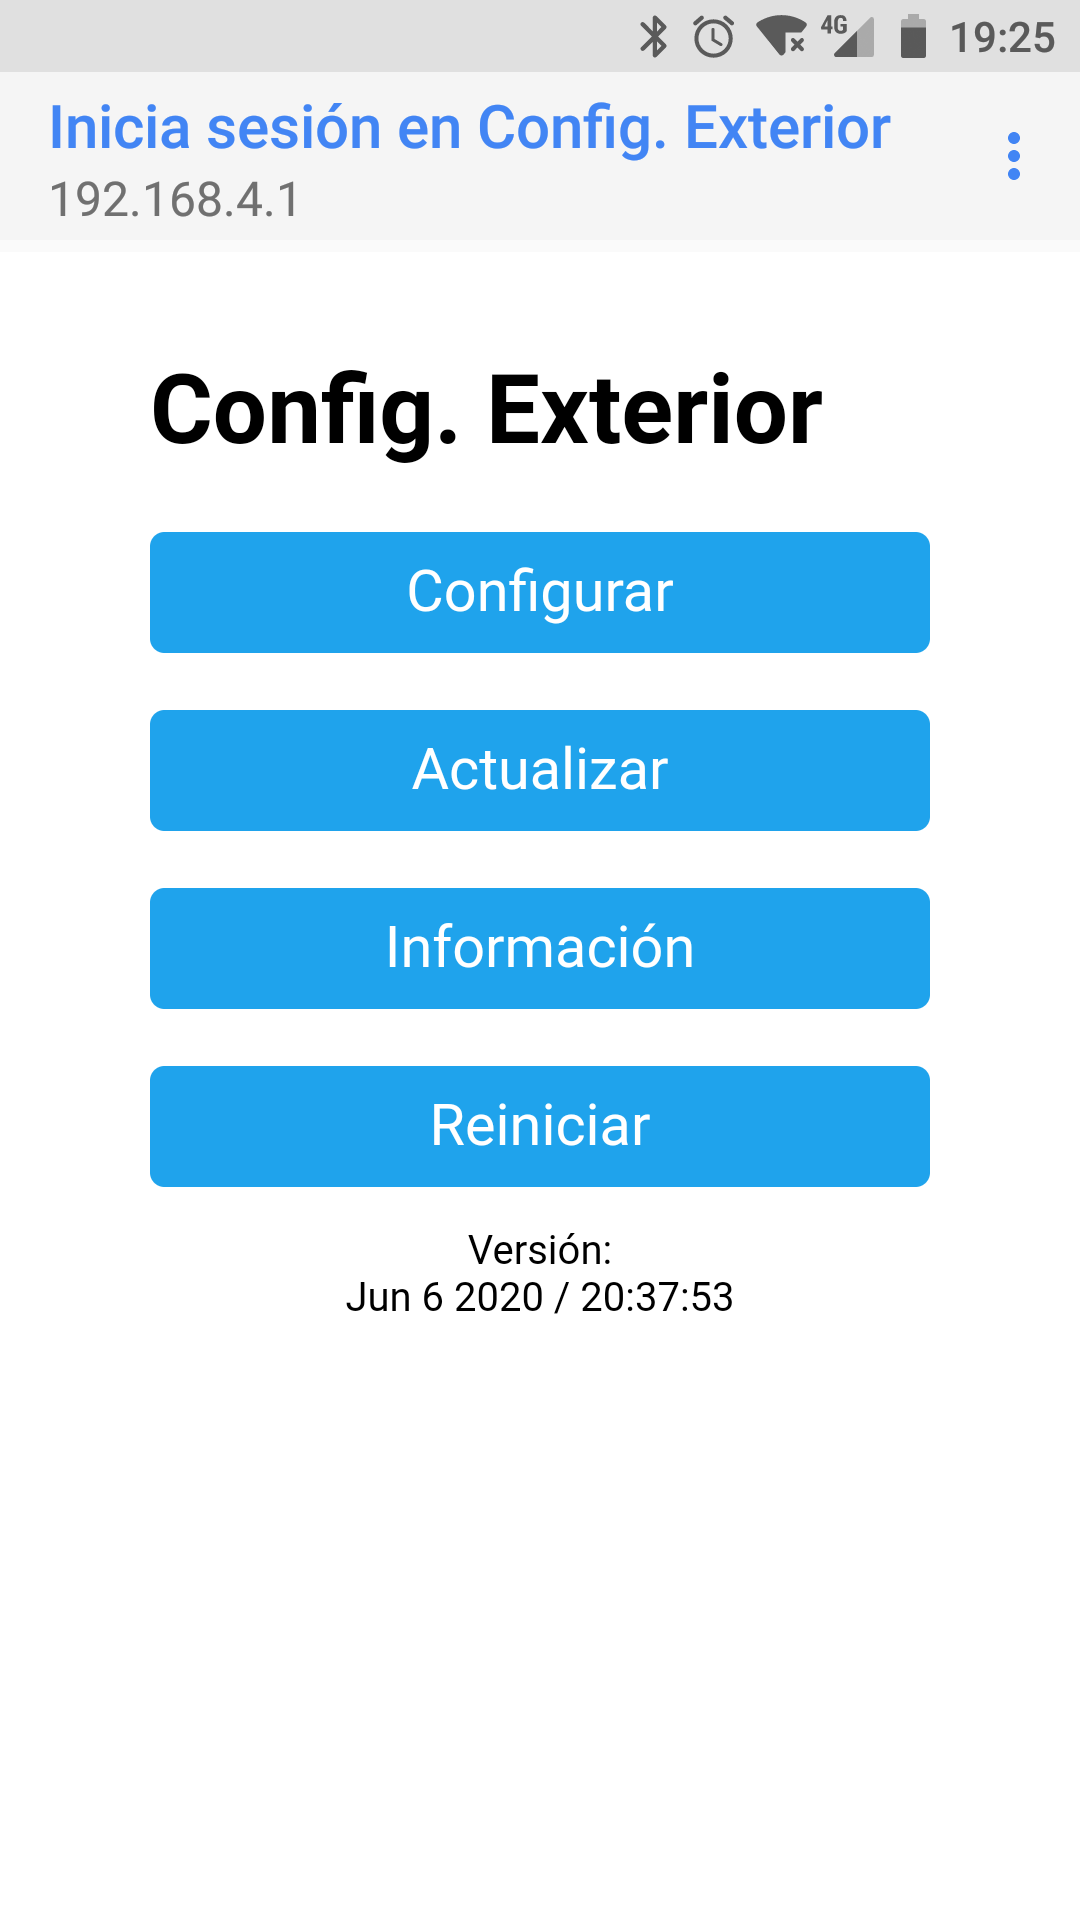
\includegraphics[width=1\columnwidth,frame]{images/exterior-menu}
  \caption{}
  \label{fig:exterior-menu}
\end{subfigure}
\caption{Menú de gestión de los módulos interior (a) y exterior (b)}
\label{fig:menu}
\end{figure}

\subsection{Opciones de gestión}

La figura~\ref{fig:menu} muestra las opciones de gestión que ofrecen ambos módulos:

\begin{descriptioncompact}

\item[Configurar] --- Permite establecer diversos parámetros de funcionamiento, como el nombre de host, la frecuencia de actualizaciones, el horario de silencio, \etc Las opciones de configuración se describen en la sección~\ref{sec:config}.

\item[Actualizar] --- Permite actualizar el firmware de los distintos módulos sin necesidad de conectarlos físicamente a un ordenador mediante una conexión USB. El proceso de actualización se detalla en la sección~\ref{sec:actualizar}.

\item[Información] --- Muestra información básica del sistema y el hardware de los módulos. La información disponible se describe en la sección~\ref{sec:info}.

\item[Reiniciar] --- Reinicia el sistema sin guardar los cambios. La sección~\ref{sec:reinicio} describe el proceso de reinicio.

\end{descriptioncompact}

Finalmente, en la parte inferior de la figura~\ref{fig:menu} se muestra la información de compilación (fecha y hora) del software del \CMS.

\subsubsection{Parámetros de configuración}
\label{sec:config}

En esta sección se detallan los diversos parámetros que se pueden configurar tanto para el \MIE como para el \MEE cuando se selecciona en el menú principal la opción \emph{Configurar}.

\importantbegin{Acceso a los parámetros de configuración}
Sea paciente mientras se carga la página que permite ajustar los parámetros de configuración. Puede tardar unos segundos ya que se deben escanear las redes wifi disponibles al alcance de los módulos.
\importantend

Las figuras~\ref{fig:interior-config} y \ref{fig:exterior-config} muestran el aspecto que tiene la interfaz de configuración para el \MI y el \ME respectivamente. Cuando se ha terminado de establecer la configuración deseada, es necesario pulsar en el botón \emph{Guardar} que se encuentra al final de la interfaz de configuración. En tal caso, se mostrarán los mensajes de confirmación de la figura~\ref{fig:config-saved} según proceda, y el módulo recién configurado se reiniciará. En caso de no desear guardar los cambios, es posible volver atrás y reiniciar el módulo (ver sección~\ref{sec:reinicio}) sin alterar la configuración previa.

\begin{figure}
\begin{subfigure}{0.49\columnwidth}
  \centering
  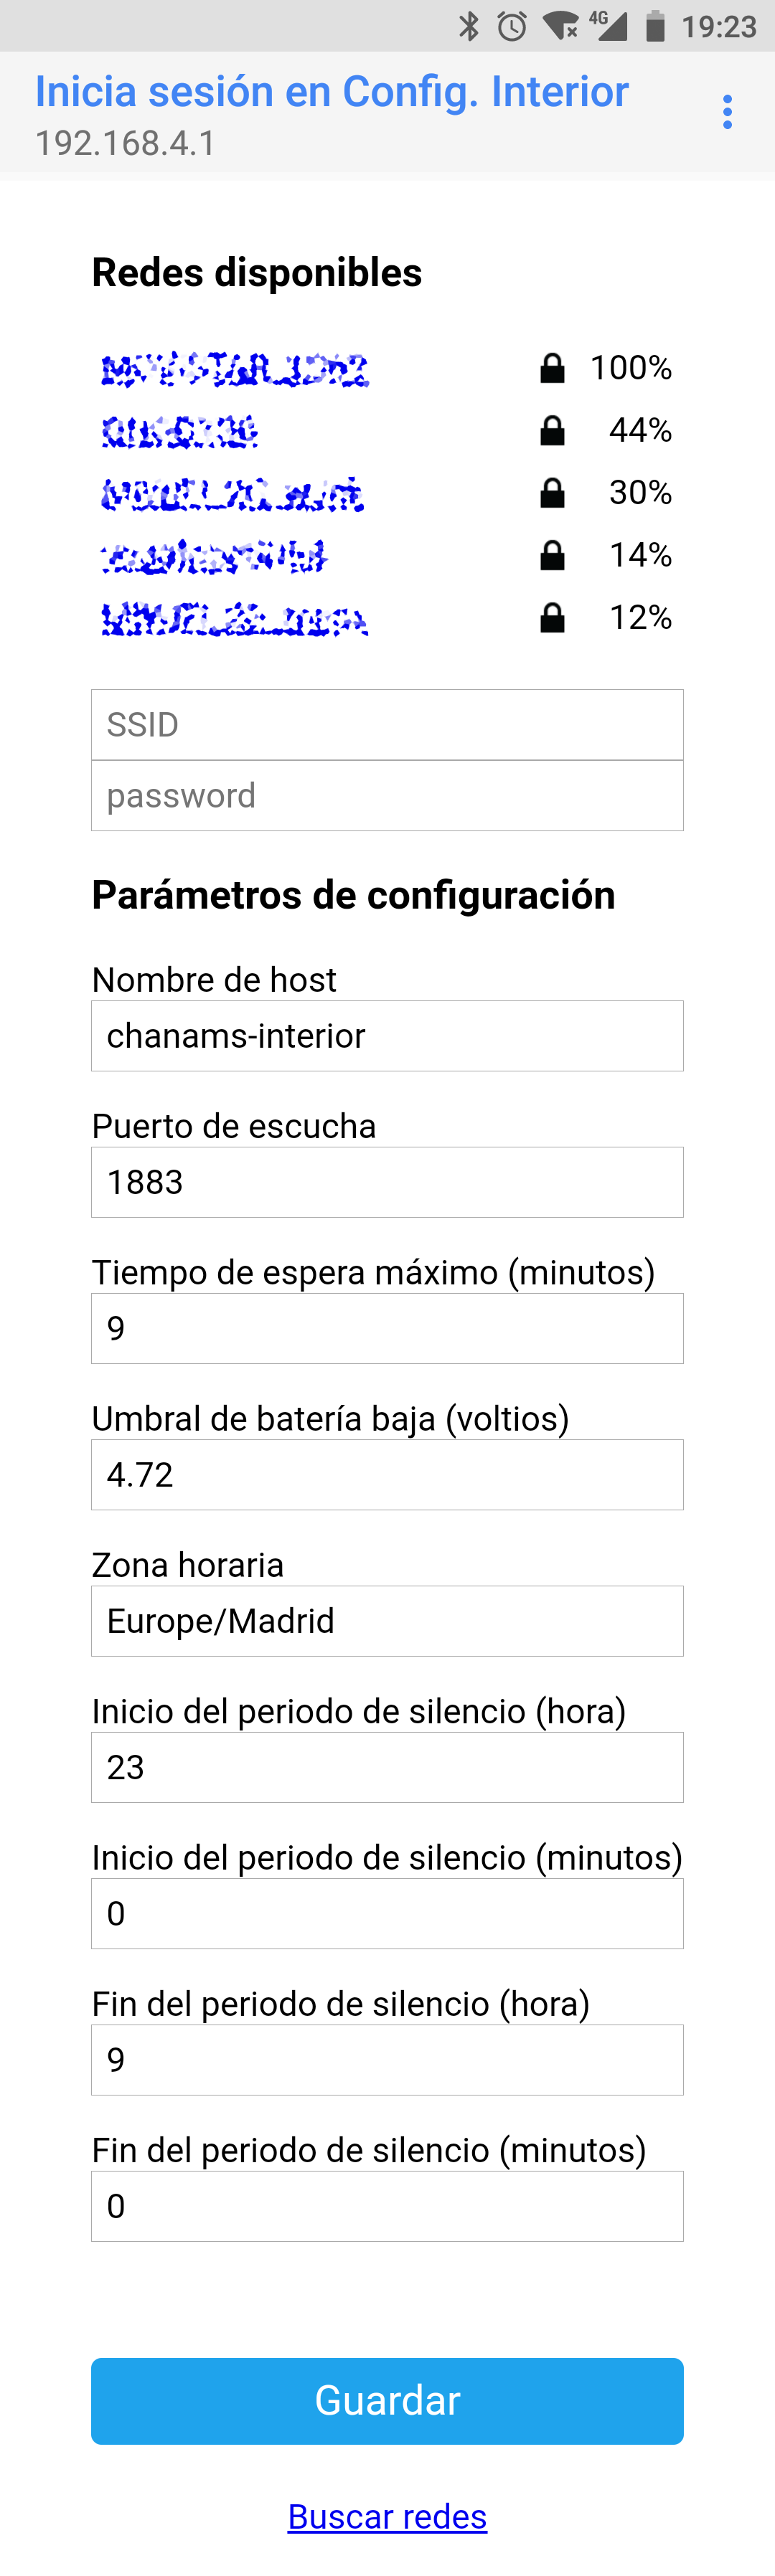
\includegraphics[height=0.94\textheight,frame]{images/interior-config}
  \caption{}
  \label{fig:interior-config}
\end{subfigure}
\hfill
\begin{subfigure}{0.49\columnwidth}
  \centering
  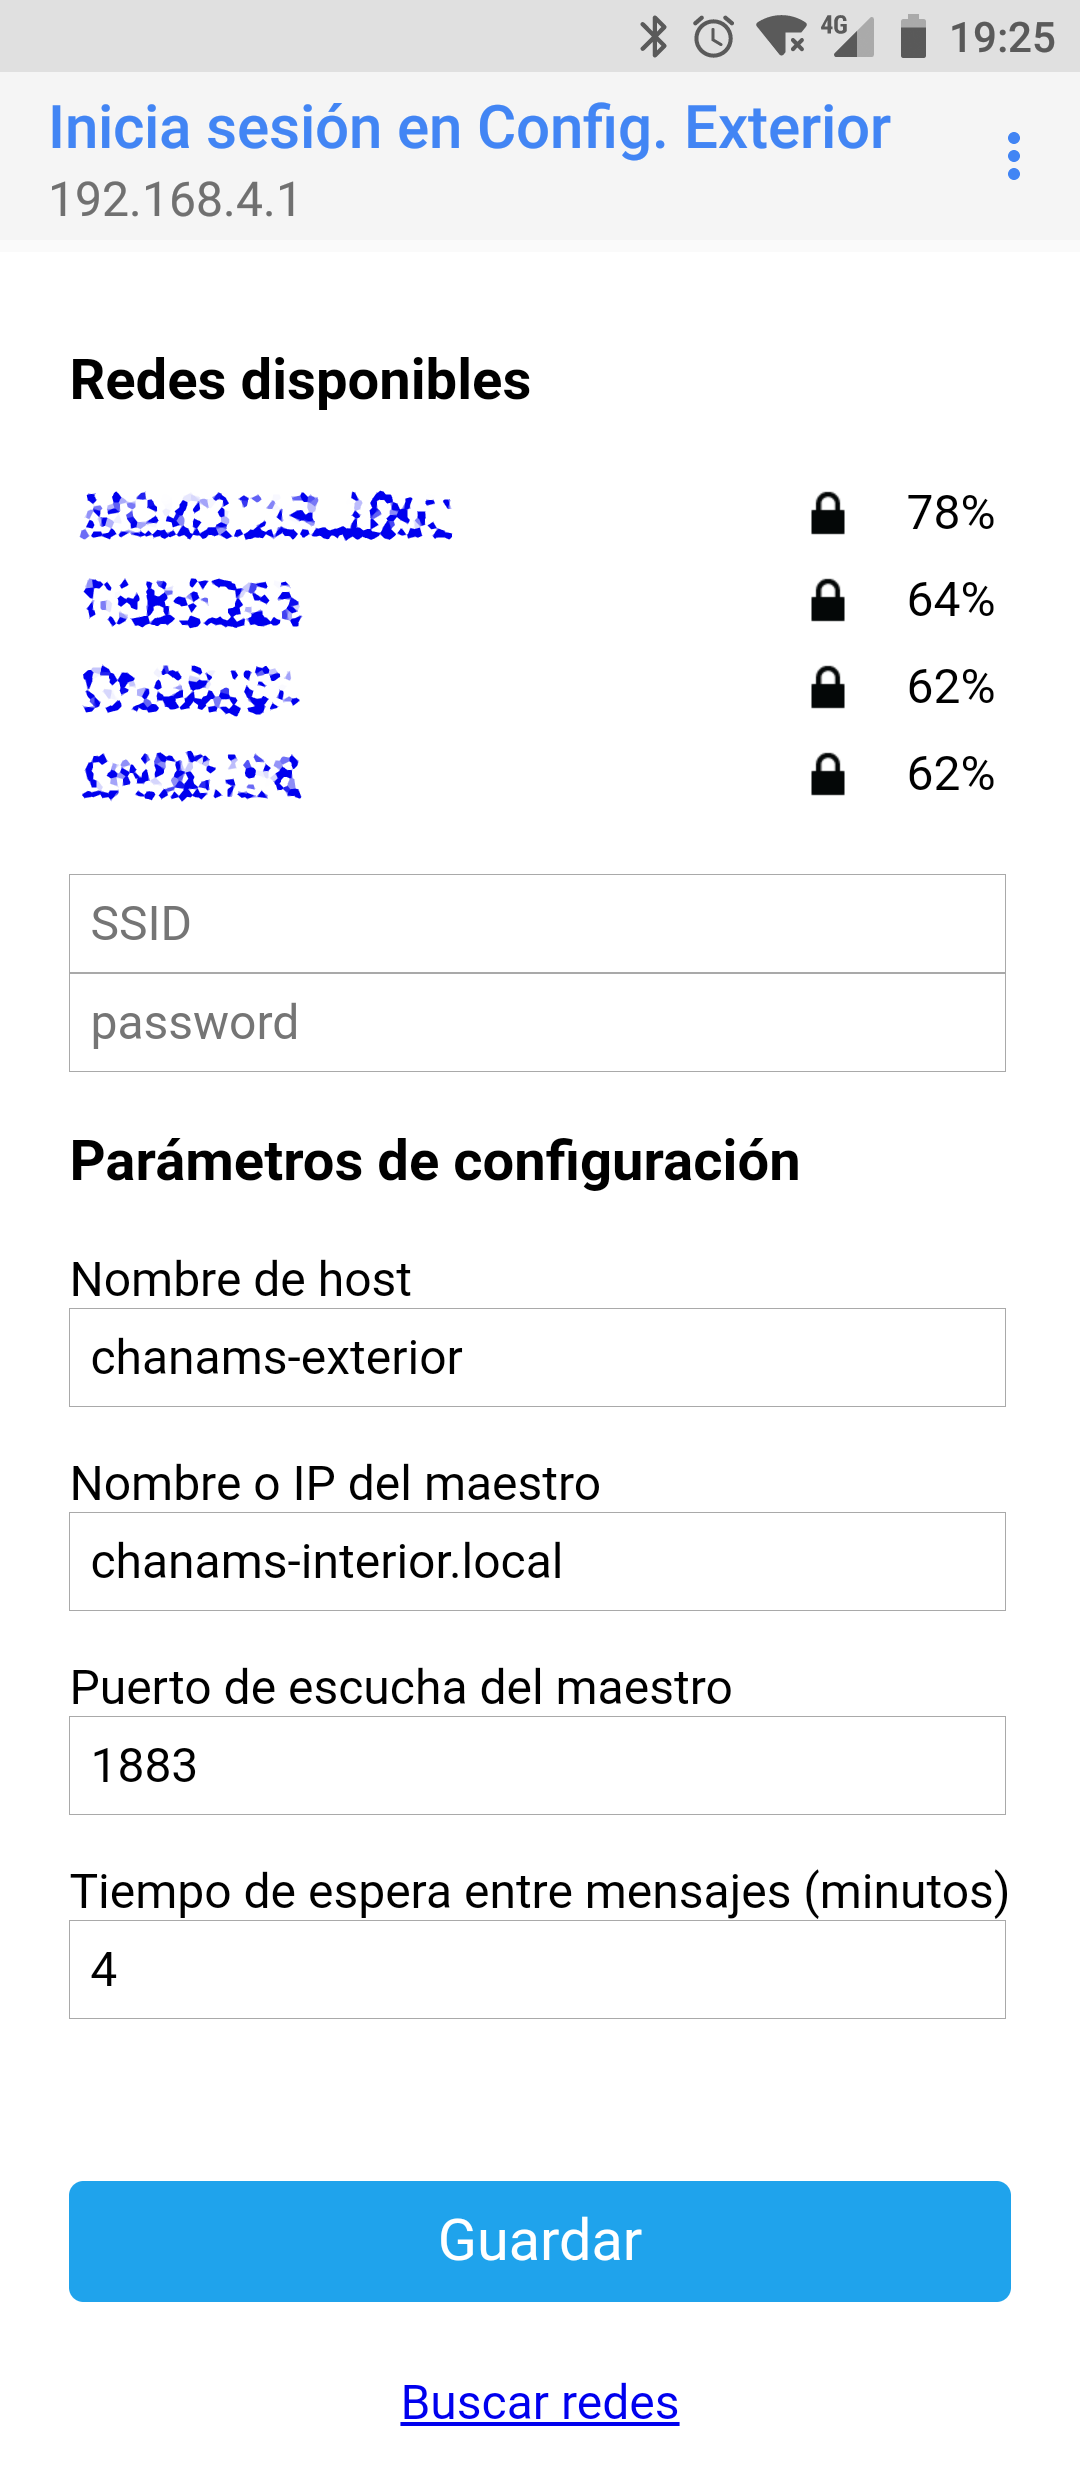
\includegraphics[width=0.9\columnwidth,frame]{images/exterior-config}
  \caption{}
  \label{fig:exterior-config}
\end{subfigure}
\caption{Configuración de los módulos interior (a) y exterior (b)}
\end{figure}

\begin{figure}
\begin{subfigure}{0.49\columnwidth}
  \centering
  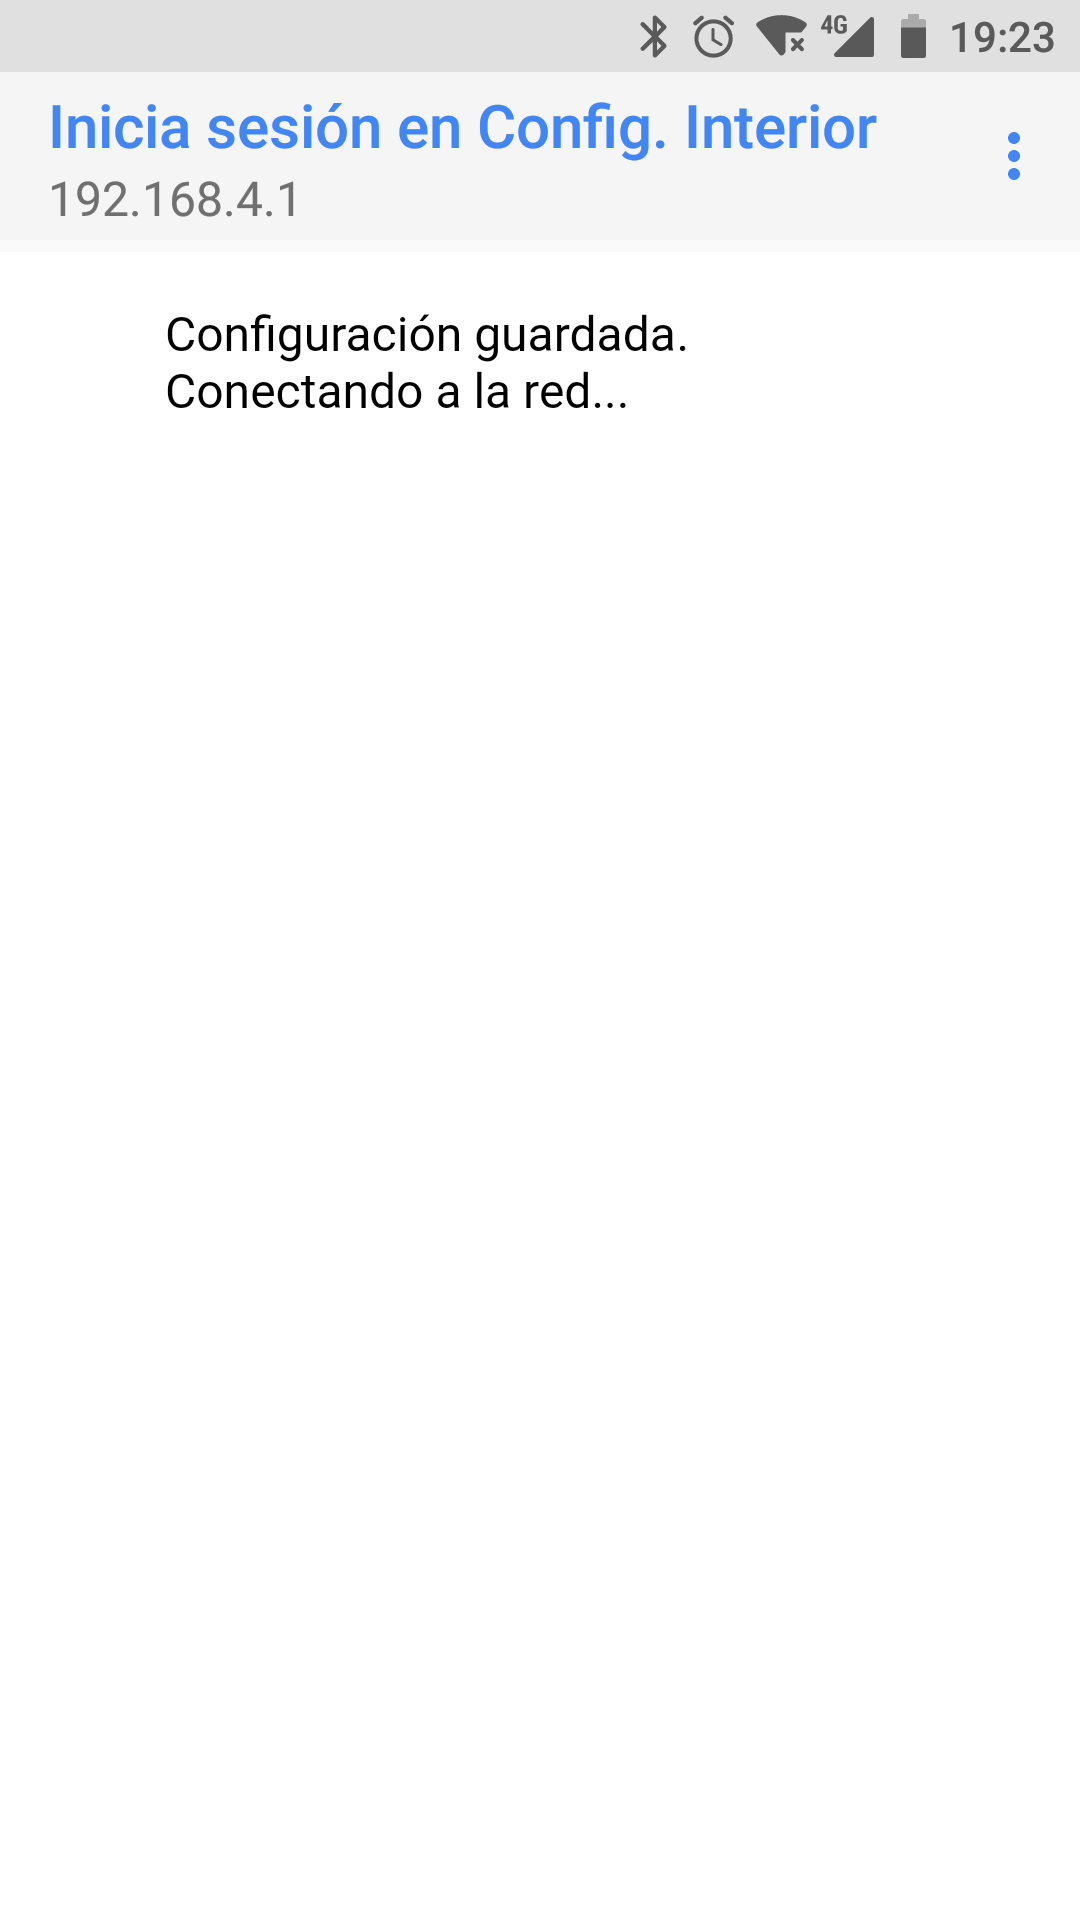
\includegraphics[width=1\columnwidth,frame]{images/interior-config-saved}
  \caption{}
  \label{fig:interior-config-saved}
\end{subfigure}
\hfill
\begin{subfigure}{0.49\columnwidth}
  \centering
  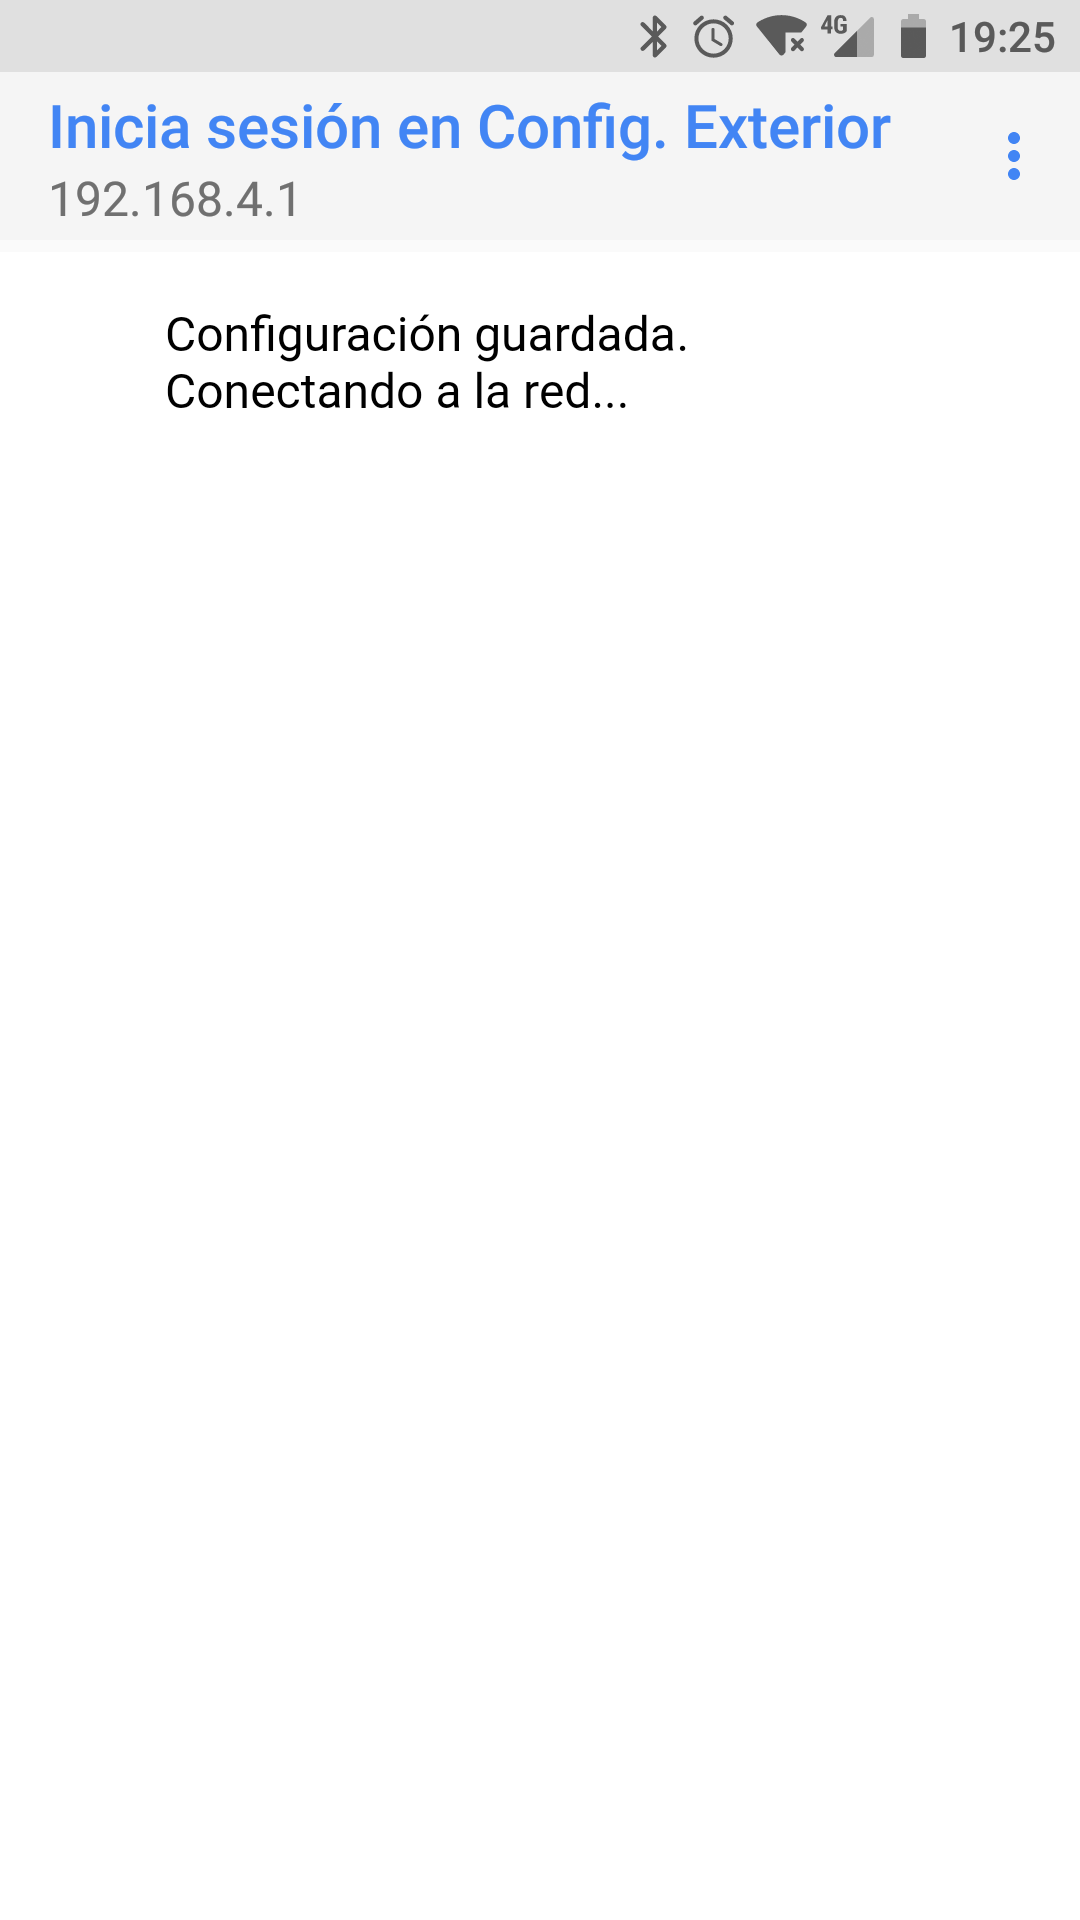
\includegraphics[width=1\columnwidth,frame]{images/exterior-config-saved}
  \caption{}
  \label{fig:exterior-config-saved}
\end{subfigure}
\caption{Mensaje de confirmación de configuración guardada en los módulos interior (a) y exterior (b)}
\label{fig:config-saved}
\end{figure}


\paragraph{Redes disponibles}

Como ya se ha avanzado en la sección~\ref{sec:inicio-rapido} (\textit{\nameref{sec:inicio-rapido}}), la sección \emph{Redes disponibles} permite establecer el nombre y la contraseña de la red wifi a la que se conectarán los módulos del \CMS. El establecimiento de la configuración de red wifi se hace de forma similar tanto en el \MIE como en el \MEE. 

\paragraph{Parámetros de configuración del \textit{módulo interior}}
\label{sec:params-interior}

\begin{description}

  \item[Nombre de host] --- Nombre que anunciará el \MIE como su nombre de host. Los dispositivos que soporten el protocolo mDNS podrán resolver la dirección IP del \MI empleando el nombre DNS \texttt{nombre-de-host\allowbreak.\allowbreak\-lo\-cal} (por ejemplo, \texttt{chanams-interior.local}). El nombre de host sólo puede contener letras mayúsculas (\texttt{A..Z}), minúsculas (\texttt{a..z}), números (\texttt{0..9}) y \mbox{guiones~(\texttt{-})}.
  
  Valor por defecto: \texttt{chanams-interior}
  
  \item[Puerto de escucha] --- Puerto de escucha del broker MQTT alojado en el \MIE.

  Valor por defecto: \texttt{1883}
  
  \item[Tiempo de espera máximo (minutos)] --- Tiempo máximo en minutos que el \MIE debe esperar entre dos mensajes del \MEE. Cuando dicho tiempo se excede sin que el \MI haya recibido comunicación por parte del \ME, se considerará que la conexión se ha perdido y se disparará la \emph{alarma de conexión perdida} (ver sección~\ref{sec:alarmas}, \textit{\nameref{sec:alarmas}}, y tabla~\ref{tab:luces}).
  
  Valor por defecto: \texttt{16}
  
  \tipbegin{Estableciendo un tiempo de espera máximo}
  Dada la naturaleza del protocolo de comunicación entre el \MEE y el \MIE, no es extraño que la comunicación entre ambos se pierda puntualmente perdiéndose algunos mensajes. Por tanto, se recomienda que el \emph{Tiempo de espera máximo} del \MIE sea al menos 3 veces (o incluso más) el \emph{Tiempo de espera entre mensajes} del \MEE (ver sección~\ref{sec:params-exterior} a continuación) más un minuto extra.
  
  Así, el valor por defecto se calcula como (5 $\times$ 3) $+$ 1 $=$ 16, donde 5 es el \emph{Tiempo de espera entre mensajes}, y 16 el \emph{Tiempo de espera máximo} resultante.
  
  En todo caso, el \emph{Tiempo de espera máximo} debe ser inferior al tiempo que puede pasar el depósito exterior sin supervisión y sin rebosar cuando se encuentra cerca de su límite de capacidad.
  \tipend
  
  
  \item[Umbral de batería baja (voltios)] --- Valor en voltios ---decimales separados por punto (\texttt{.})--- a partir del cual se considerará que la batería del \MEE está lo suficientemente baja como baja para lanzar los \emph{avisos de batería baja}  (ver sección~\ref{sec:alarmas}, \textit{\nameref{sec:alarmas}}).
  
  Valor por defecto: \texttt{4.72}
  
  \tipbegin{Ajuste del umbral de batería baja}
  El valor por defecto del \emph{Umbral de batería baja} está ajustado según los datos experimentales recogidos en el anexo~\ref{app:curva-descarga}. No obstante, puede ser deseable tanto incrementar como decrementar este umbral.
  
  Por ejemplo, a medida que las baterías se degradan, la caída en el voltaje es más pronunciada y rápida acortando el tiempo entre el \emph{aviso de batería baja} y la \emph{alarma de conexión perdida} (ver sección~\ref{sec:alarmas}, \textit{\nameref{sec:alarmas}}). Ajustando este umbral a un valor más alto se puede incrementar el tiempo entre el \emph{aviso} y la \emph{alarma}.
  
  Igualmente, con baterías en perfectas condiciones, puede desearse incrementar el tiempo entre el \emph{aviso de batería baja} y la \emph{alarma de conexión perdida} si el \emph{Tiempo de espera entre mensajes} (ver sección~\ref{sec:params-exterior}) se ha establecido a un intervalo muy largo, ya que en tal caso podrían pasar días o semanas entre uno y otro.
  \tipend
  
  \item[Zona horaria] --- Nombre de la zona horaria\footnote{Véase \url{https://en.wikipedia.org/wiki/List_of_tz_database_time_zones} para la lista de zonas horarias estándar.} donde se encuentra instalado el \CMS. Sirve para ajustar automáticamente el reloj interno del \MEE a la hora local a partir de la hora universal UTC. El reloj interno también se ajustará automáticamente al horario de verano o invierno si es necesario.
  
  Valor por defecto: \texttt{Europe/Madrid}

  \item[Inicio del periodo de silencio (hora)] e~~{\color{main}\uppercase{Inicio del periodo de silencio (minutos)}} --- Estos dos parámetros de configuración permiten establecer la hora y minutos (incluídos) a partir de los cuales el \CMS no emitirá avisos sonoros (ver sección~\ref{sec:alarmas}, \textit{\nameref{sec:alarmas}}). 
  
  
  Valor por defecto (hora): \texttt{23}
  
  Valor por defecto (minutos): \texttt{0}
  
  \item[Fin del periodo de silencio (hora)] y~~{\color{main}\uppercase{Fin del periodo de silencio (minutos)}}~--- Estos dos parámetros de configuración permiten establecer la hora y minutos (excluídos) a partir de los cuales el \CMS emitirá avisos sonoros (ver sección~\ref{sec:alarmas}, \textit{\nameref{sec:alarmas}}).
  
  Valor por defecto (hora): \texttt{9}
  
  Valor por defecto (minutos): \texttt{0}
  
  \attbegin{Ejemplo de periodo de silencio}
  Tomando como referencia los valores por defecto para el \emph{Inicio del periodo de silencio} y el \emph{Fin del periodo de silencio}, el \CMS no emitirá ningún sonido entre las 23:00 y las 08:59.
  \attend
\end{description}

\paragraph{Parámetros de configuración del \textit{módulo exterior}}
\label{sec:params-exterior}

\begin{description}

  \item[Nombre de host] --- Nombre que anunciará el \MEE como su nombre de host. El nombre de host puede contener únicamente letras mayúsculas (\texttt{A..Z}), minúsculas (\texttt{a..z}), números (\texttt{0..9}) y \mbox{guiones~(\texttt{-})}. Nótese que, aunque los dispositivos que soportan el protocolo mDNS podrían teóricamente resolver la dirección IP del \ME empleando el nombre DNS \texttt{nombre-de-host\allowbreak.\allowbreak\-lo\-cal} (por ejemplo, \texttt{chanams-exterior.local}), en la práctica, el \ME pasa la mayor parte del tiempo en reposo y con el enlace wifi desconectado.
  
  Valor por defecto: \texttt{chanams-exterior}
  
  \item[Nombre o IP del módulo interior] --- Nombre DNS o IP del \MIE. Si se emplea un nombre DNS ---el \MEE soporta el protocolo mDNS--- puede emplearse el \emph{Nombre de host} que se describe en la sección~\ref{sec:params-interior} (\textit{\nameref{sec:params-interior}}) añadiéndole el sufijo \texttt{.local}.
  
  Valor por defecto: \texttt{chanams-interior.local}
  
  \item[Puerto de escucha del módulo interior] --- Puerto de escucha del broker MQTT alojado en el \MIE. Debe conincidir con el \emph{Puerto de escucha} que se describe en la sección~\ref{sec:params-interior} (\textit{\nameref{sec:params-interior}}).

  Valor por defecto: \texttt{1883}
  
  \item[Tiempo de espera entre mensajes (minutos)] --- Tiempo que el \MEE debe permanecer en reposo entre comprobaciones del nivel de depósito del agua y el resto de sensores. A mayor tiempo de espera del \ME, mayor será la duración de la batería.
  
  No obstante, ha de considerarse que el \emph{Tiempo de espera entre mensajes} está relacionado con el \emph{Tiempo de espera máximo} (ver sección~\ref{sec:params-interior}, \textit{\nameref{sec:params-interior}}), que a su vez debe ser inferior al tiempo máximo que el depósito puede permanecer sin supervisión cuando está cercano a su máxima capacidad. Se recomienda que el \emph{Tiempo de espera entre mensajes} sea al menos 3 veces menor que el \emph{Tiempo de espera máximo}. Esto permitiría la pérdida de 3 mensajes por causas normales entre el \ME y el \MI sin que salten las alarmas. 

  Valor por defecto: \texttt{5}
   
\end{description}


\subsubsection{Actualización remota}
\label{sec:actualizar}

\begin{figure}
\begin{subfigure}{0.49\columnwidth}
  \centering
  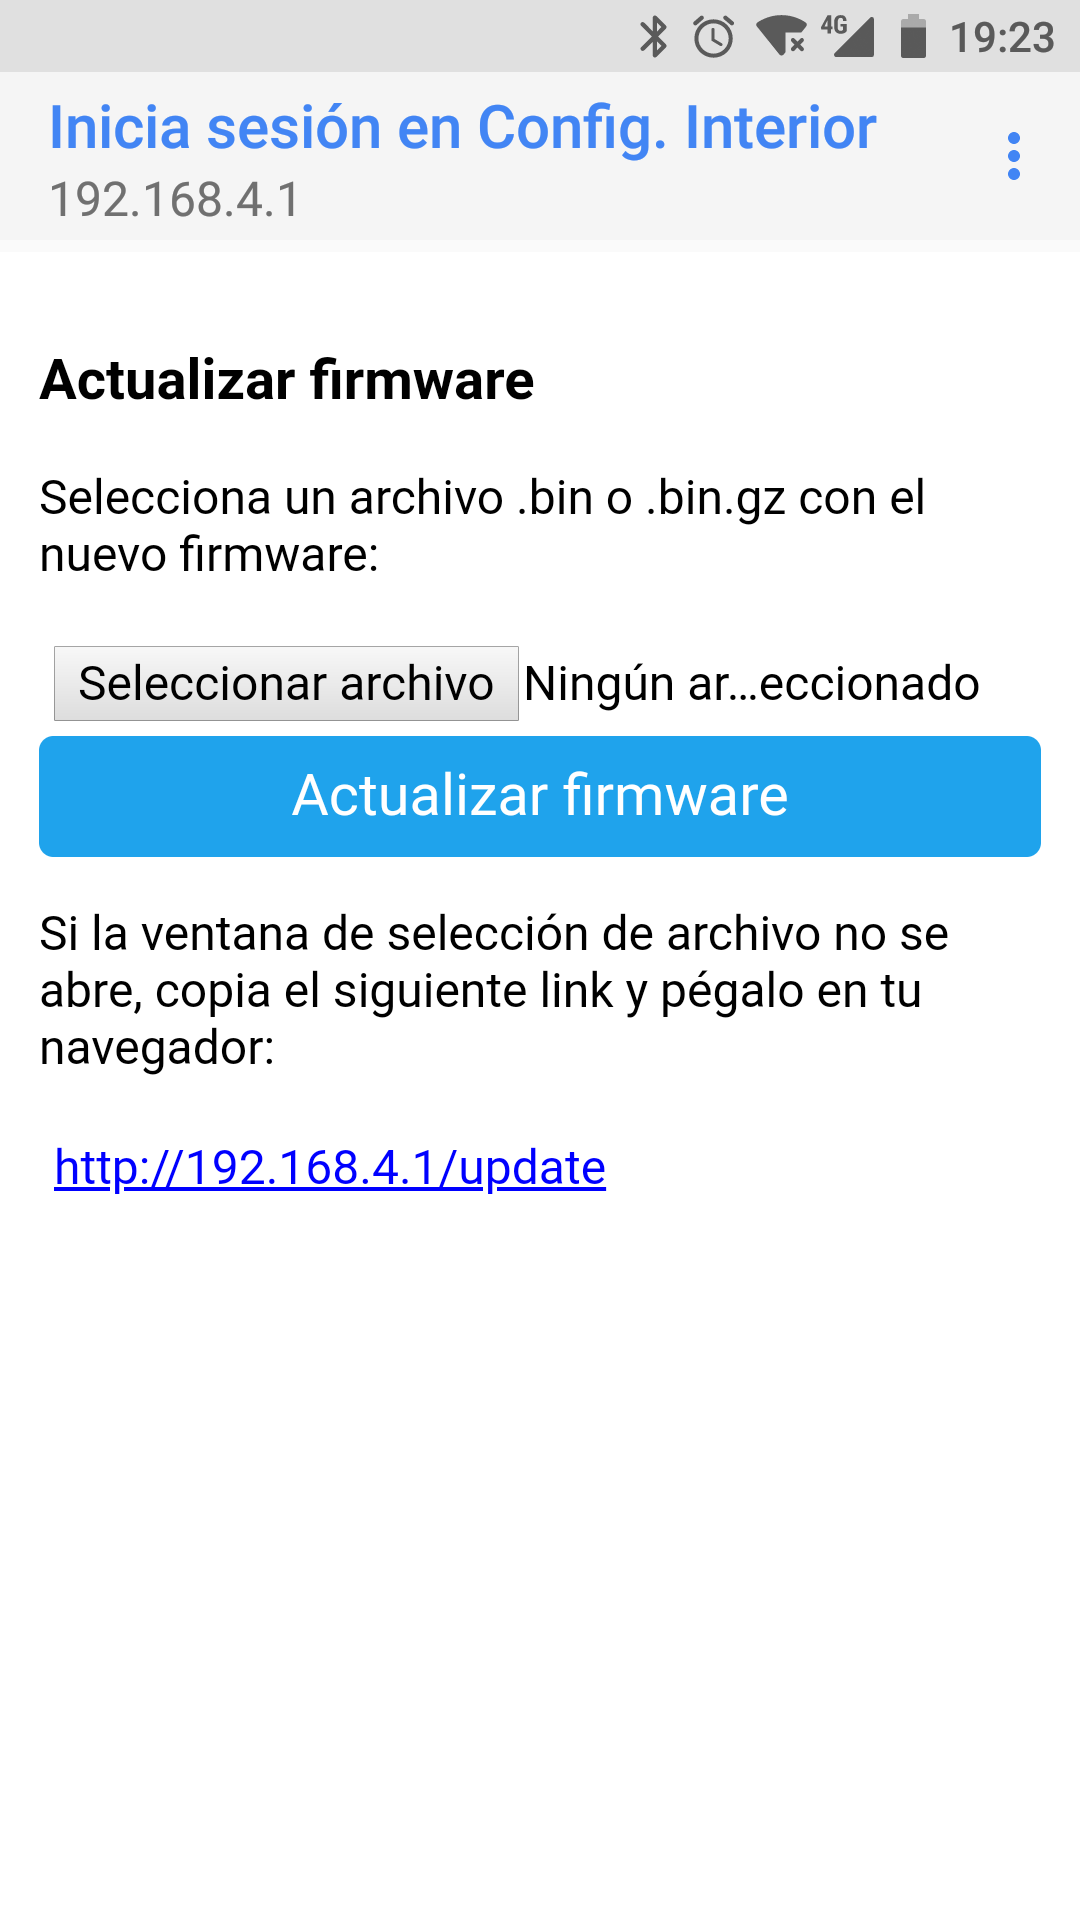
\includegraphics[width=1\columnwidth,frame]{images/interior-firmware-update}
  \caption{}
  \label{fig:interior-firmware-update}
\end{subfigure}
\hfill
\begin{subfigure}{0.49\columnwidth}
  \centering
  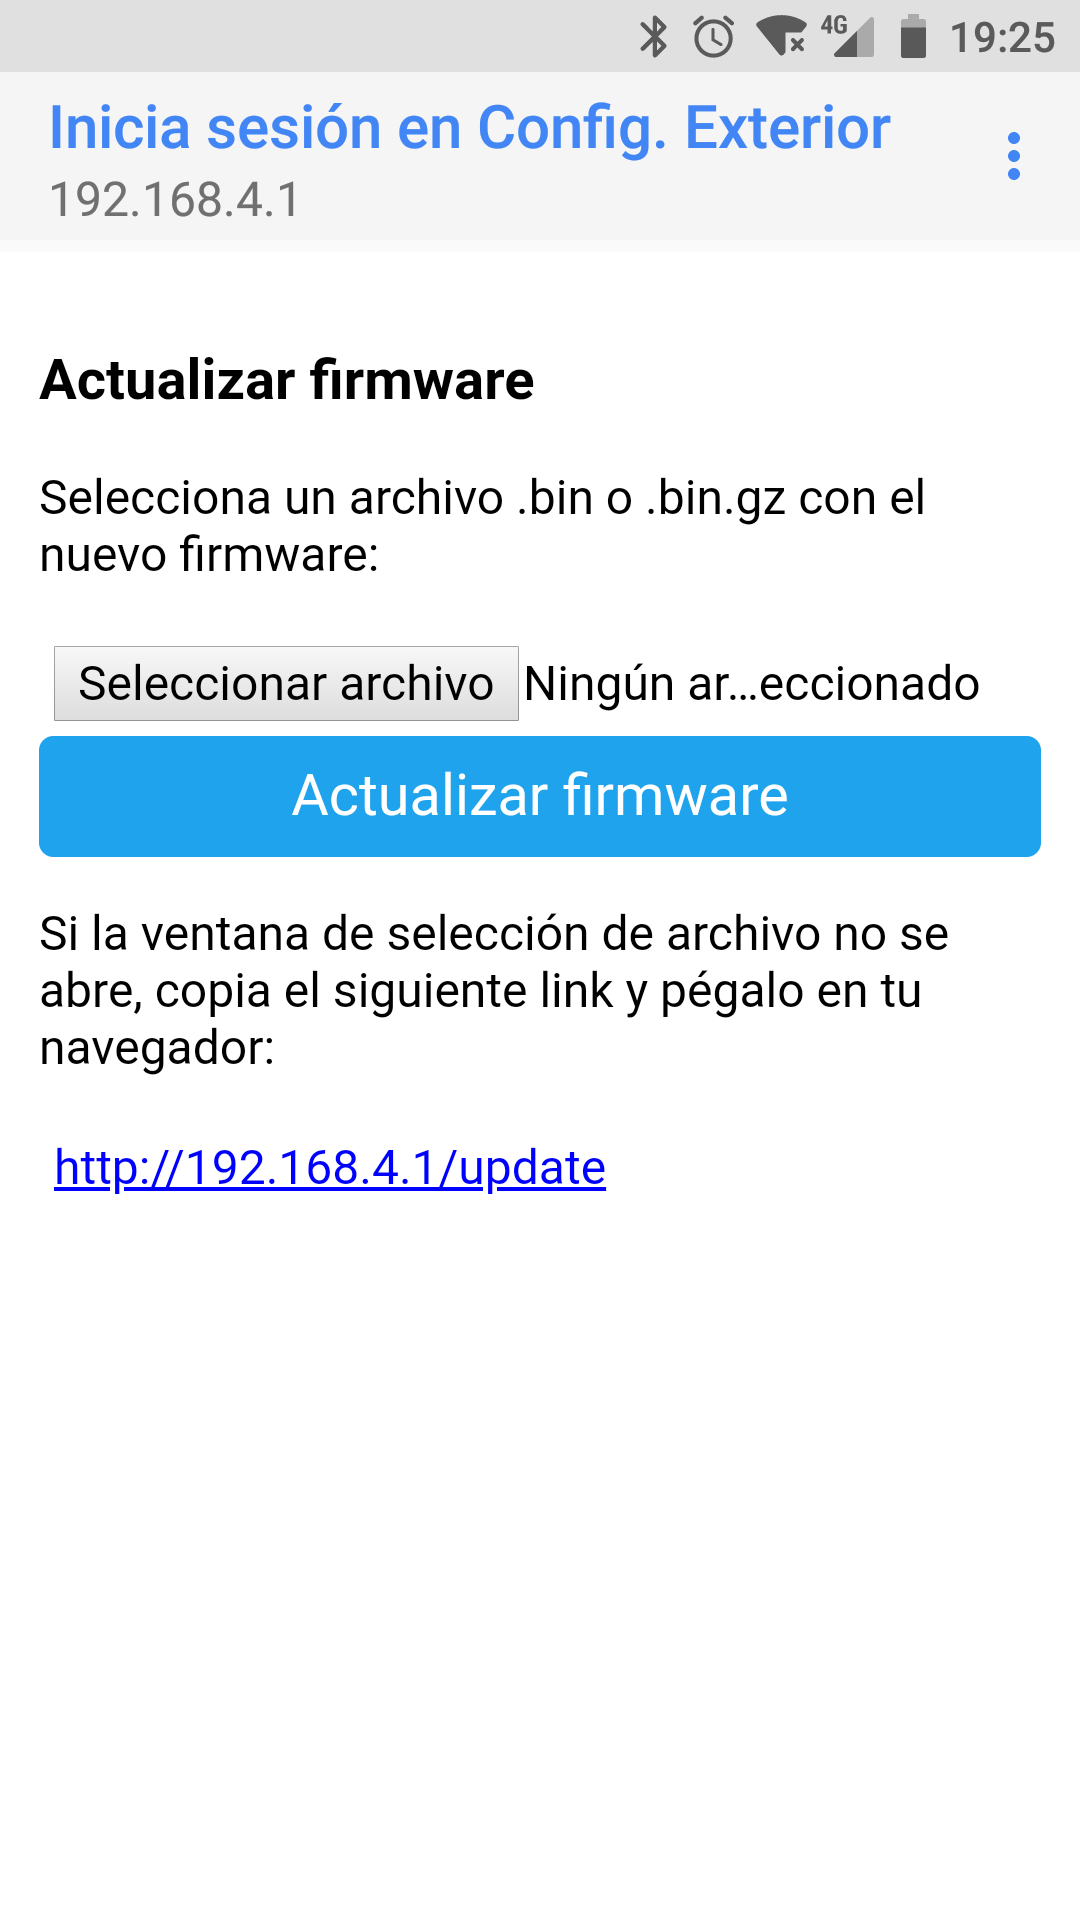
\includegraphics[width=1\columnwidth,frame]{images/exterior-firmware-update}
  \caption{}
  \label{fig:exterior-firmware-update}
\end{subfigure}
\caption{Actualización del firmware de los módulos interior (a) y exterior (b)}
\label{fig:firmware-update}
\end{figure}

\begin{figure}
\begin{subfigure}{0.32\columnwidth}
  \centering
  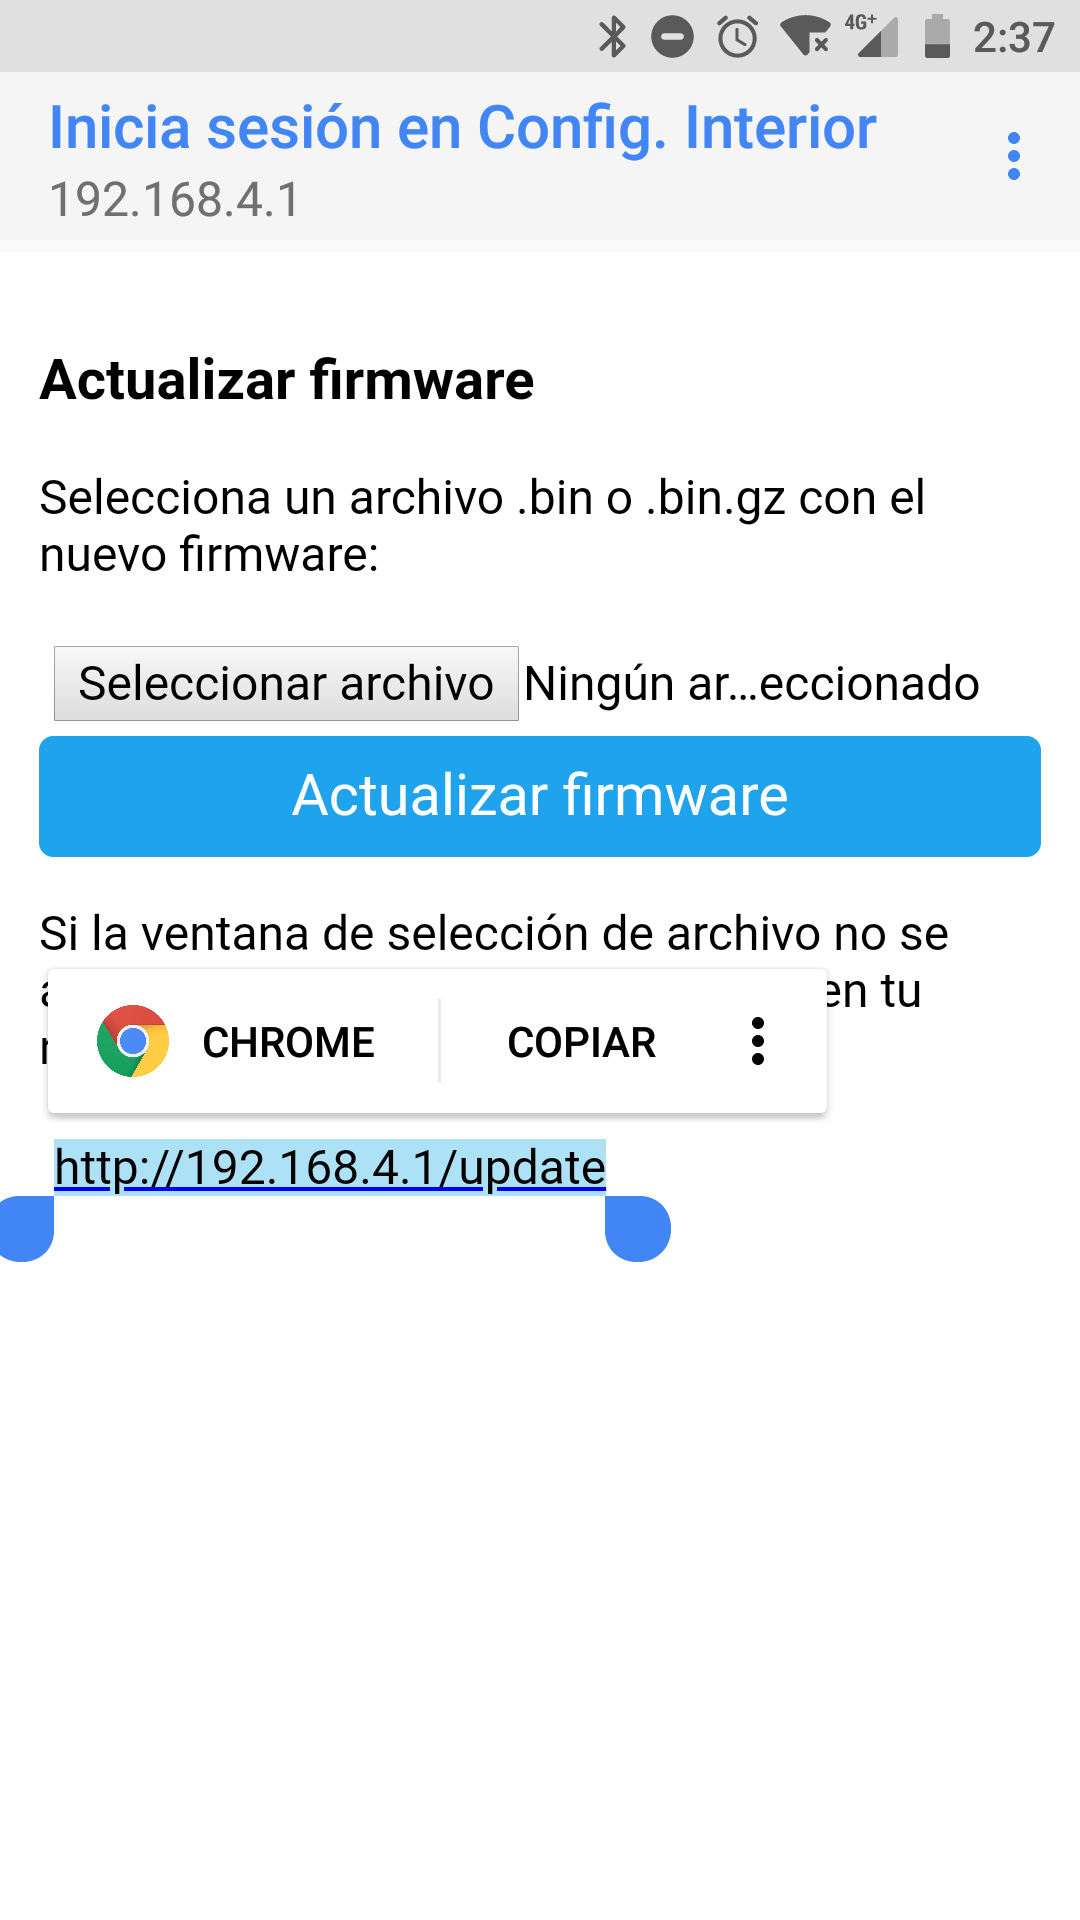
\includegraphics[width=1\columnwidth,frame]{images/interior-firmware-update-selection}
  \caption{}
  \label{fig:interior-firmware-update-selection}
\end{subfigure}
\hfill
\begin{subfigure}{0.32\columnwidth}
  \centering
  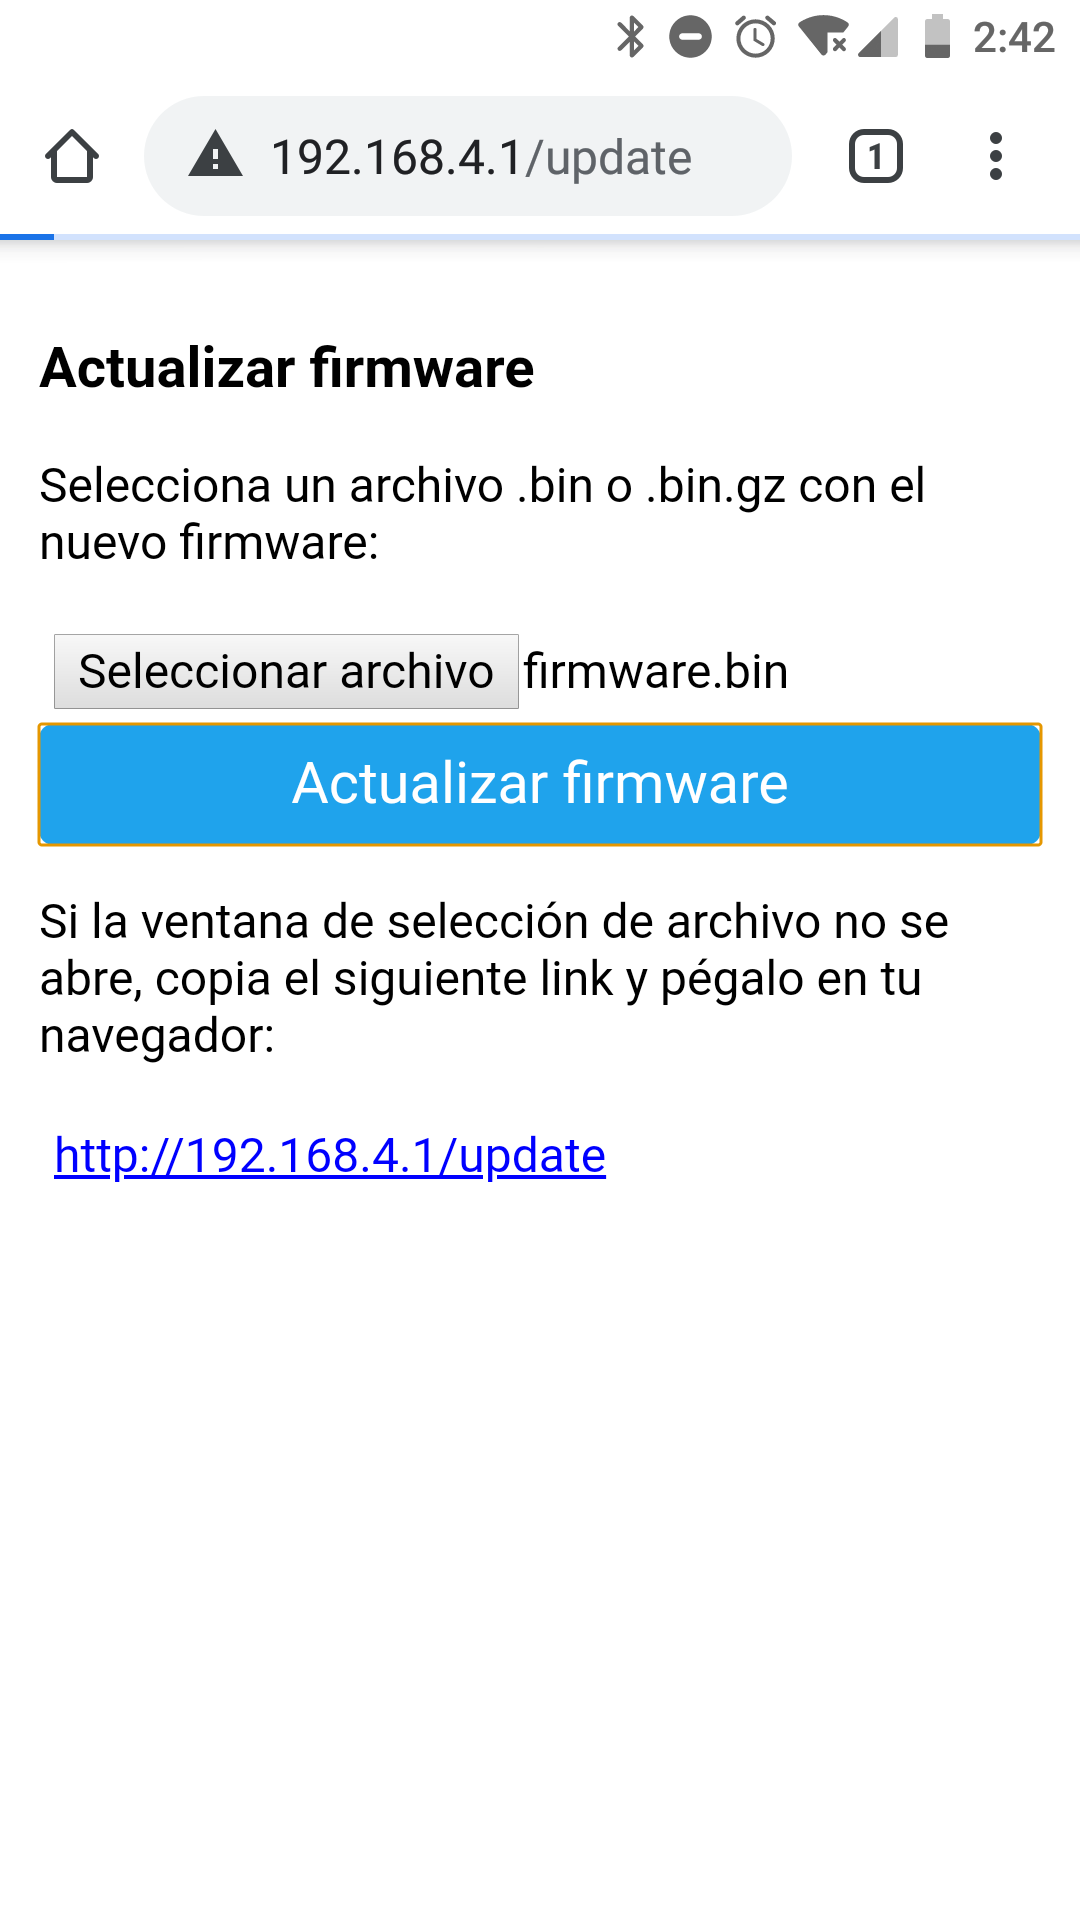
\includegraphics[width=1\columnwidth,frame]{images/interior-firmware-update-chrome}
  \caption{}
  \label{fig:interior-firmware-update-chrome}
\end{subfigure}
\hfill
\begin{subfigure}{0.32\columnwidth}
  \centering
  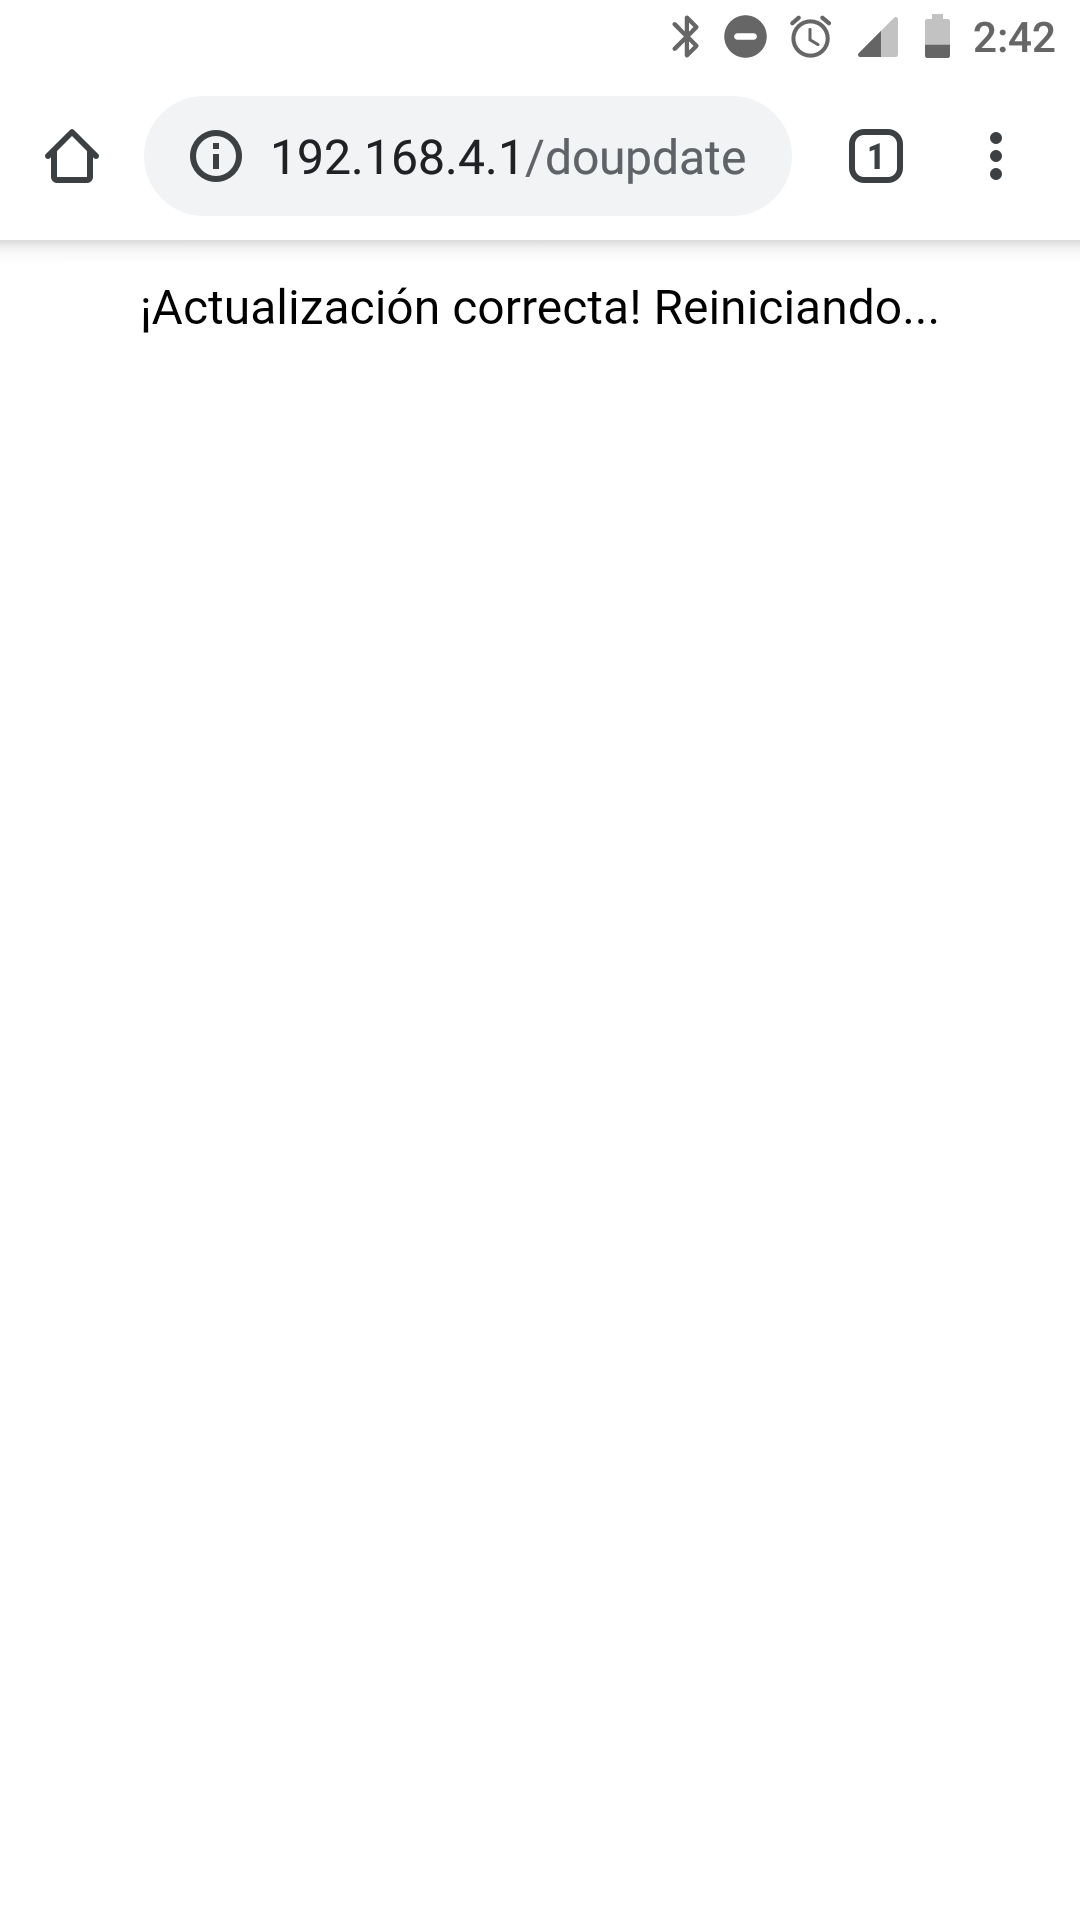
\includegraphics[width=1\columnwidth,frame]{images/interior-firmware-update-done}
  \caption{}
  \label{fig:interior-firmware-update-done}
\end{subfigure}
\caption{Actualización del firmware: (a) acceder desde el navegador, (b) seleccionar el fichero .bin, (c) confirmación de actualización correcta}
\label{fig:firmaware-update-browser}
\end{figure}

Es posible actualizar el software tanto del \MIE como del \MEE de forma remota a partir de la opción \emph{Actualizar} (ver figura~\ref{fig:firmware-update}). Para ello, se deberá disponer de una imagen del firmware actualizado en formato de fichero binario (\texttt{.bin}).

Para ello, se ha de pulsar sobre \emph{Seleccionar archivo}, seleccionando el fichero del firmware actualizado (por ejemplo, \texttt{firmware.bin}). La actualización se aplica pulsando en \emph{Actualizar software}. La actualización se ejecuta en unos pocos segundos, y al finalizar, el módulo se reinicia.


\attbegin{Actualizando en portal cautivo en un dispositivo móvil}
Si accede a la interfaz de actualización desde la interfaz de portal cautivo de un dispositivo móvil, es posible que el botón de \emph{Seleccionar archivo} se encuentre deshabilitado. En tal caso, deberá acceder a la interfaz de actualización desde un navegador web estándar tal y como muestra la figura~\ref{fig:firmaware-update-browser}.


\textbf{Para poder acceder a la interfaz de gestión desde un navegador web ---como \textit{Google Chrome}--- desde su dispositivo móvil, es probable que deba desactivar previamente su conexión de datos.}


En primer lugar (figura~\ref{fig:interior-firmware-update-selection}), deberá seleccionar y copiar la dirección de la interfaz web de actualización. A continuación (figura~\ref{fig:interior-firmware-update-chrome}), deberá ir al navegador web de sus dispositivo ---como Google Chrome--- y pegar la dirección en la barra de direcciones. En este punto, ya podrá hacer uso de los botones de la interfaz y proceder a seleccionar el archivo \texttt{firmware.bin} con normalidad. Por último, tras pulsar \emph{Actualizar firmware}, el módulo informará del resultado de la actualización y se reiniciará (figura~\ref{fig:interior-firmware-update-done}). Este proceso es el mismo tanto para el \MIE como para el \MEE.
\attend

\subsubsection{Información del sistema}
\label{sec:info}

La sección de \emph{Información} muestra información interna del hardware y del sistema que controlan tanto el \MIE como el \MEE. La informaciónque se muestra es:



\begin{description}

  \item[Chip id] --- Identificador del chip ESP8266 como un entero de 32 bits.

  \item[Flash Chip id] --- Identificador del chip de la memoria flash como un entero de 32 bits.
   
  \item[IDE Flash Size] --- Tamaño de la memoria flash, en bytes, tal y como lo percibe el SDK (puede ser menor que el tamaño real).
   
  \item[Real Flash Size] --- Tamaño real de la memoria flash, en bytes, basado en el identificador del chip de la memoria flash.
  
  \item[Soft AP IP] --- Dirección IP del punto de acceso por software que permite conectarse al módulo que se encuentra en modo gestión.
   
  \item[Soft AP MAC] --- Dirección MAC del punto de acceso por software.
   
  \item[Station MAC] --- Dirección MAC de la estación wifi del chip ESP8266.
   
\end{description}

\vfill

\begin{figure}[b!]
\begin{subfigure}{0.49\columnwidth}
  \centering
  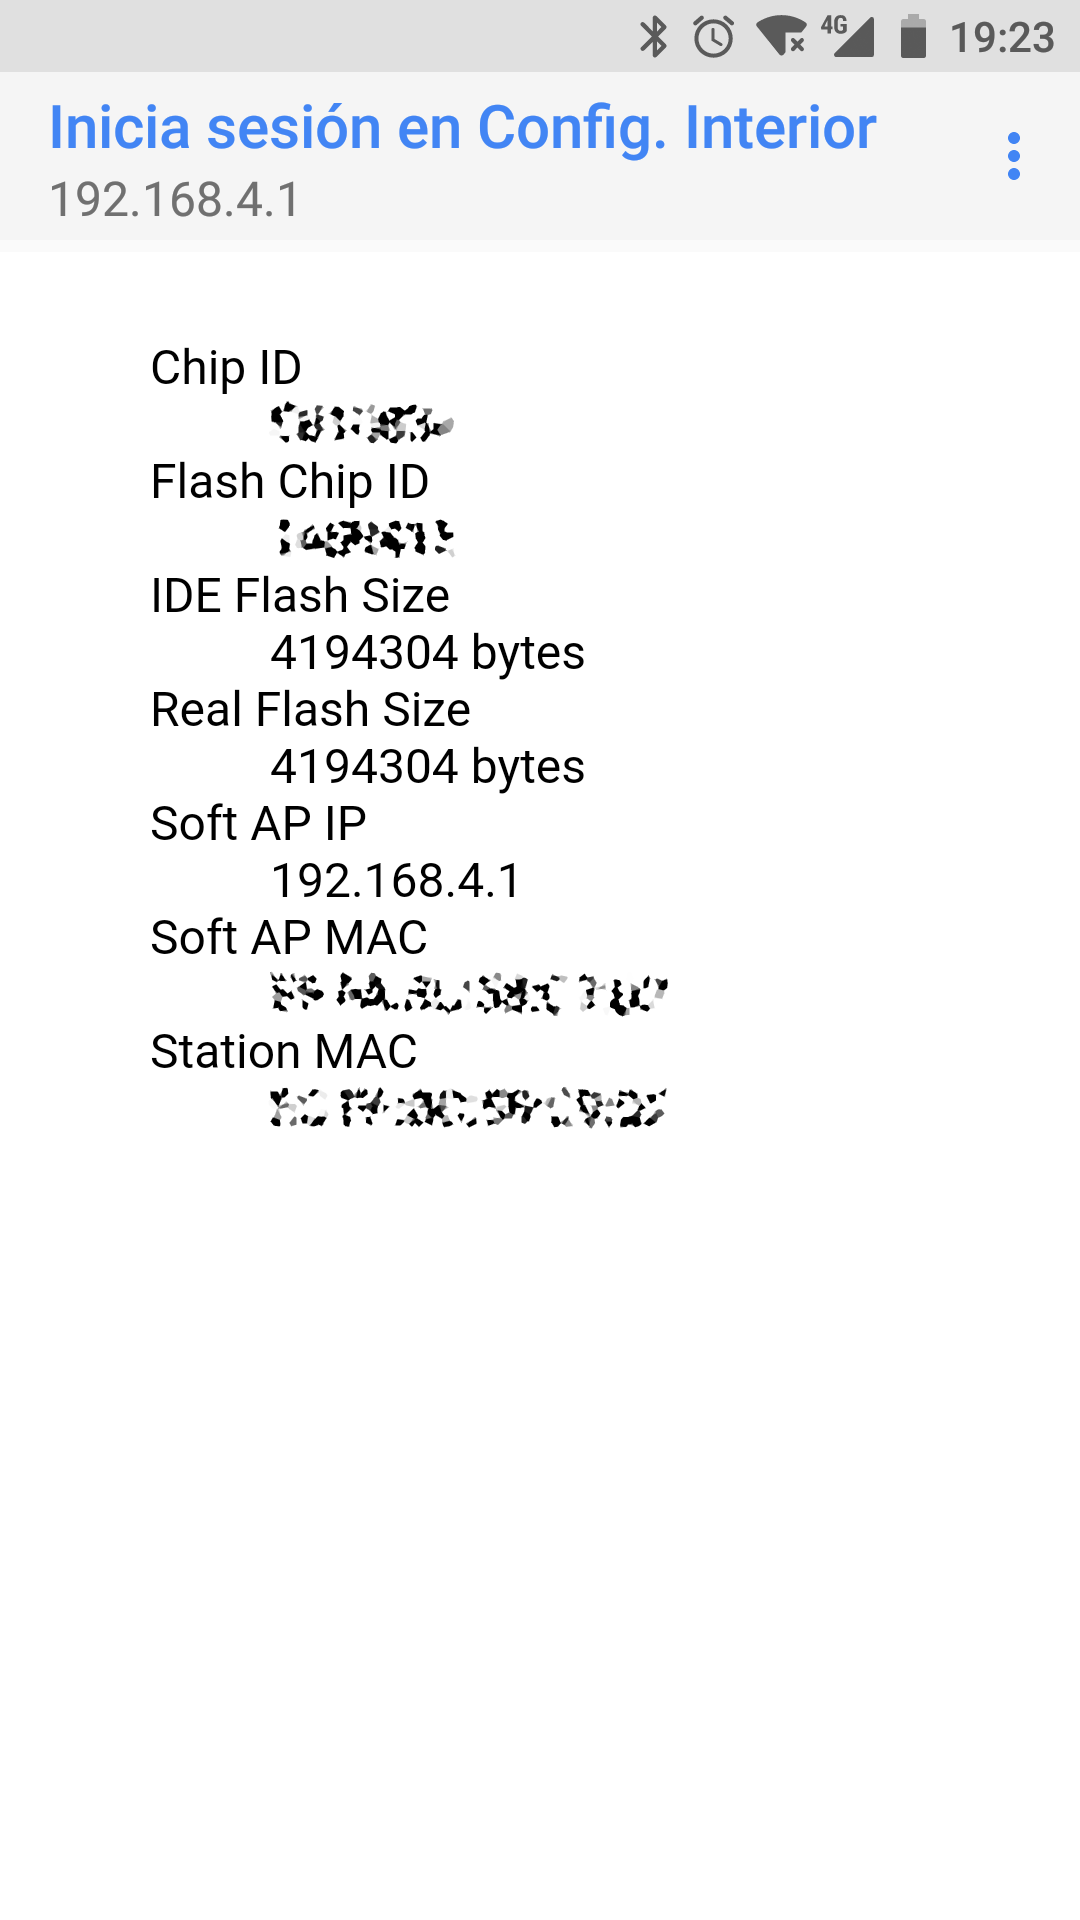
\includegraphics[width=1\columnwidth,frame]{images/interior-info}
  \caption{}
  \label{fig:interior-info}
\end{subfigure}
\hfill
\begin{subfigure}{0.49\columnwidth}
  \centering
  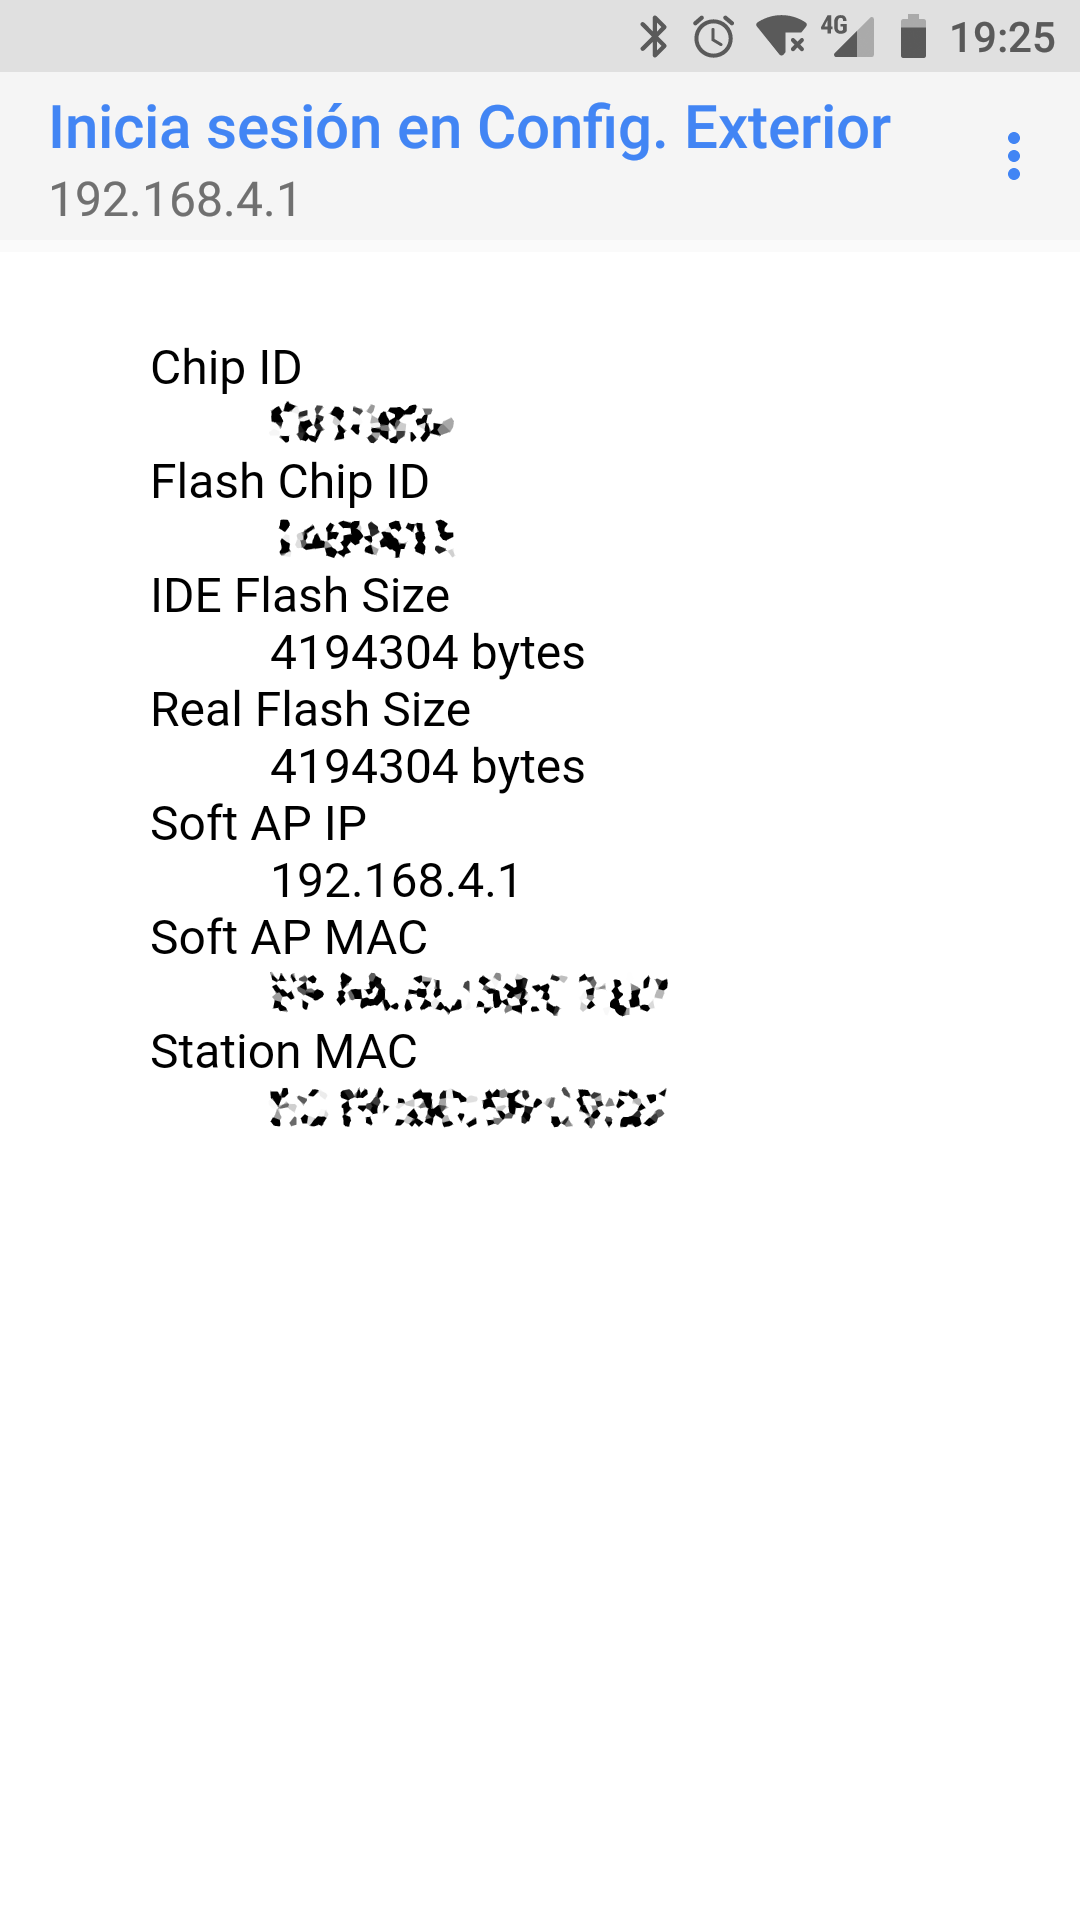
\includegraphics[width=1\columnwidth,frame]{images/exterior-info}
  \caption{}
  \label{fig:exterior-info}
\end{subfigure}
\caption{Información de los módulos interior (a) y exterior (b)}
\label{fig:info}
\end{figure}

\clearpage

\subsubsection{Reinicio}
\label{sec:reinicio}

Al pulsar la opción \emph{Reiniciar}, el sistema se reinicia directamente sin realizar ningún cambio en la configuración tal y como se muestra en las figuras~\ref{fig:interior-restart} y \ref{fig:exterior-restart}.

\vfill

\begin{figure}[b!]
\begin{subfigure}{0.49\columnwidth}
  \centering
  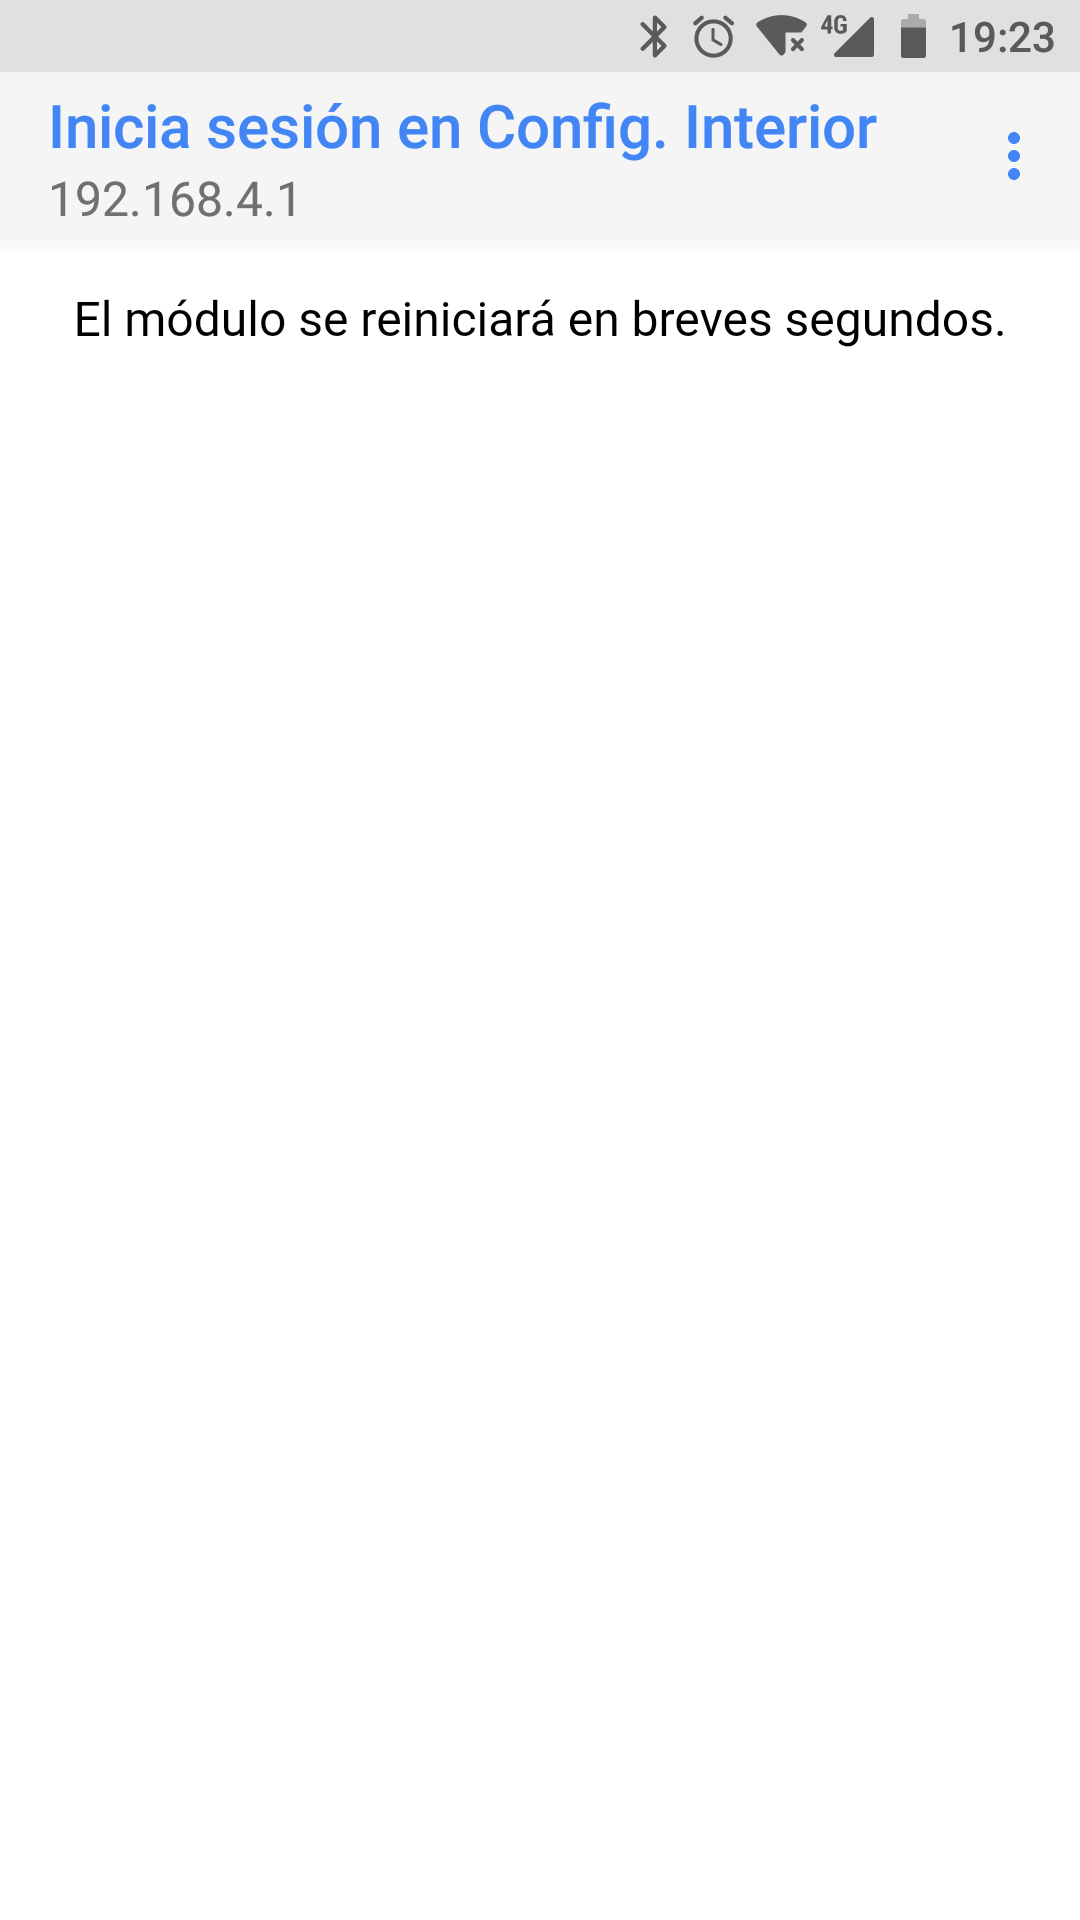
\includegraphics[width=1\columnwidth,frame]{images/interior-restart}
  \caption{}
  \label{fig:interior-restart}
\end{subfigure}
\hfill
\begin{subfigure}{0.49\columnwidth}
  \centering
  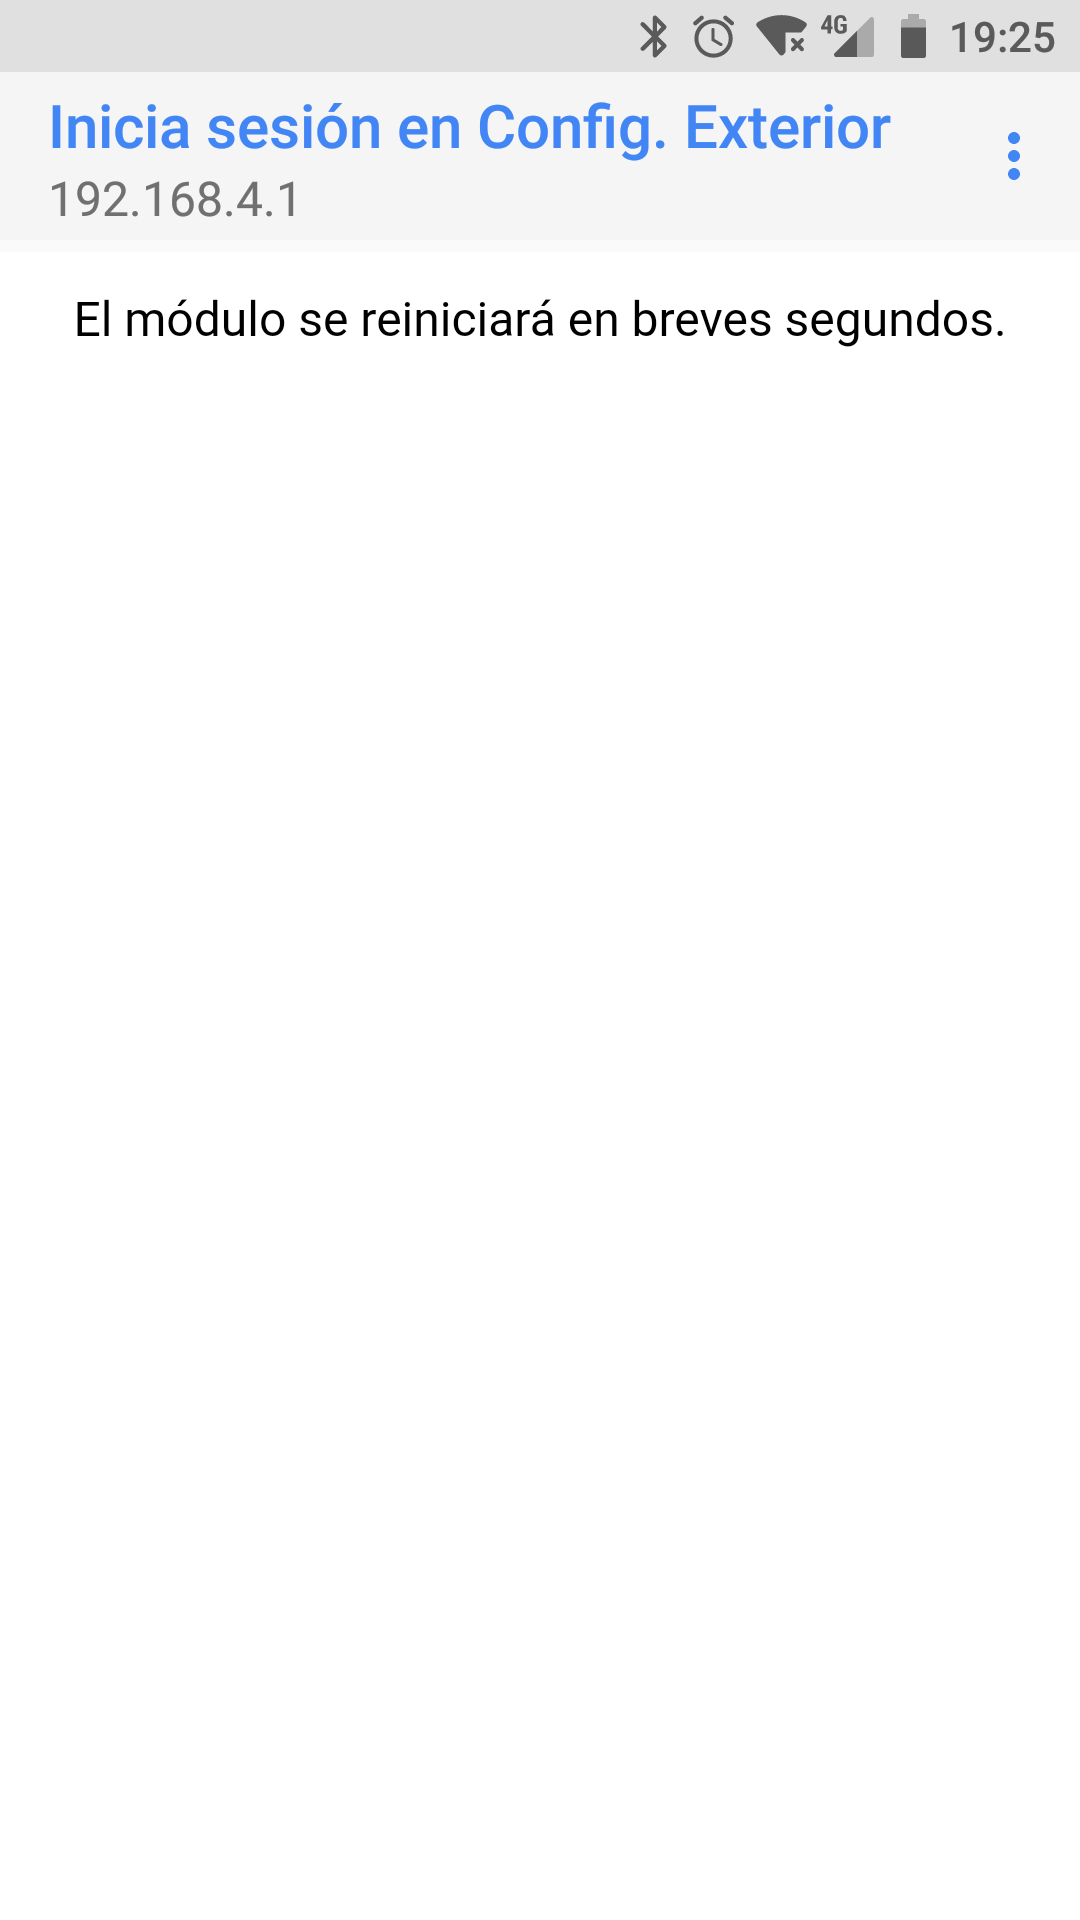
\includegraphics[width=1\columnwidth,frame]{images/exterior-restart}
  \caption{}
  \label{fig:exterior-restart}
\end{subfigure}
\caption{Reiniciando los módulos interior (a) y exterior (b)}
\label{fig:restart}
\end{figure}


\section{Resolución de problemas}
\label{sec:resolucion-problemas}

\subsection{En caso de batería baja}
\label{sec:bateria-baja}

\begin{enumeratecompact}

\item \textbf{Reemplace las baterías del \MEE.} Para ello:

\begin{itemizecompact}

\item acceda al \MEE; 
\item retire la cubierta trasera transparente;
\item retire las baterías antiguas; y finalmente,
\item coloque las nuevas siguiendo las indicaciones del portabaterías. 

\end{itemizecompact}

Una vez haya cambiado las baterías, espere a que el \MIE y el \MIE se sincronicen correctamente.  

\begin{itemizecompact}

\item Si los módulos se sincronizan, y la alarma se ha detenido, ha terminado.

\item Si los módulos se sincronizan, pero el aviso de batería baja sigue sonando, continúe en el paso 2.

\item En caso de no sincronización, siga el procedimiento que se detalla en la sección~\ref{sec:conn-perdida}.

\end{itemizecompact}

\item \textbf{Compruebe que las nuevas baterías tienen el nivel de carga correcto.} Para ello, revise el nivel de batería en la pantalla 2 del menú de información del \MIE pulsando el botón multifunción \circled{I8}. Tenga en cuenta que:

\begin{itemizecompact}

\item Unas baterías recién cargadas típicamente indican un voltaje superior a los 5,0 V cuando están en perfectas condiciones. Si el valor es menor, las baterías han comenzado a degradarse.

\item Unas baterías en buenas condiciones deben de permanecer la mayor parte del tiempo de uso en un valor alrededor de los 4,8 V -- 4,9 V.

\item Si las baterías se han cargado recientemente, y su voltaje ha caído rápidamente tras poco tiempo se uso, reemplácelas por un juego nuevo y vuelva al paso 1.

\item Si las baterías muestran valores normales, pero el aviso de batería baja continúa sonando regularmente, continúe en el paso 3.

\end{itemizecompact}

\item \textbf{Compruebe el \emph{Umbral de batería baja} configurado en el \MIE.} Para ello acceda al modo gestión siguiendo el procedimiento detallado en la sección~\ref{sec:acceso-gestion}. Un valor razonable estará típicamente entre los 4,6 V y 4,8 V aproximadamente (véase la figura~\ref{fig:discharge-curve} para poder estimar los valores adecuados). En todo caso, el valor deberá ser inferior al voltaje que las baterías del \ME reportan la mayor parte de su vida útil.

\begin{itemizecompact}

\item Si necesita ajustar el \emph{Umbral de batería baja}, siga el procedimiento detallado en la sección~\ref{sec:params-interior}.

\end{itemizecompact}

\end{enumeratecompact}



\importantbegin{No emplear pilas alcalinas}
\textbf{RECUERDE: el \MEE debe emplear 4 pilas AA recargables de NiMH de 1,2 V}. El empleo de pilas alcalinas puede provocar daños permanentes por sobretensión en el \ME. 
\importantend


\subsection{En caso de depósito lleno}
\label{sec:deposito-lleno}

\begin{enumeratecompact}

\item \textbf{Vacíe el depósito que está siendo monitorizado por el \MEE.} Para ello:

\begin{itemizecompact}

\item Acceda donde se encuentre el \MEE.

\item Retire el sensor de boya del interior del depósito.

\item Vacíe el depósito en un lugar adecuado.

\item Vuelva a colocar el depósito en su lugar, e inserte de nuevo la boya en el interior del depósito a una altura adecuada cerca del límite de su capacidad.  

\end{itemizecompact}

\item \textbf{Deje que el \MEE y el \MIE actualicen su estado.} Para ello puede (alternativamente):

\begin{enumeratecompact}
  
\item esperar a que el \MEE envíe el siguiente mensaje de sincronización según el \emph{Tiempo de espera entre mensajes} configurado; o

\item reiniciar el \MEE forzando la sincronización. Para ello, coloque el interruptor de encendido \circled{E2} en la posición \off, espere unos segundos, y vuelva a conectar el \ME moviendo el interruptur de encendido \circled{E2} a la posición~\on. En caso de no sincronización, siga el procedimiento que se detalla en la sección~\ref{sec:conn-perdida}.
  
\end{enumeratecompact}

\item \textbf{Compruebe que la alarma de depósito lleno deja de sonar.} 

\begin{itemizecompact}

\item Si la \emph{alarma de depósito lleno} ha dejado de sonar, ha terminado.

\item Si la \emph{alarma de depósito lleno} continúa sonando aunque el depósito haya sido vaciado. Compruebe que:

\begin{itemizecompact}

\item El sensor de boya está en posición vertical.

\item El flotador del sensor de boya se encuentra en la posición inferior.

\item El sensor de boya está limpio y el flotador se mueve con facilidad.

\item El cable del sensor de boya y los conectores están en buenas condiciones y libres de óxido.

\end{itemizecompact}

Una vez hechas estas comprobaciones, vuelva al paso 2.

\end{itemizecompact}

\item \textbf{Si tras haber seguido los puntos previos, la \emph{alarma de depósito lleno} continúa sonando,} existe un problema anormal con el sensor de boya. Desconecte el \CMS y llévelo a reparar.

\end{enumeratecompact}

\subsection{En caso de conexión perdida}
\label{sec:conn-perdida}
En caso de que el \CMS le alerte de que se ha perdido la conexión entre en \MIE y el \MEE, proceda de la siguiente manera:

\begin{enumeratecompact}

\item \textbf{Reinicie el \MIE}. Para ello, pulse el botón de reinicio \circled{I5} ---o alterntivamente, desconecte y reconecte pasados unos segundos la alimentación USB \circled{I6}--- y espere a que el \MI informe en la pantalla LCD \circled{I1} de que se encuentra conectado a una red wifi.

\begin{itemizecompact}

\item Si tras varios intentos el \MI no se conecta a una red wifi, entre en el modo de gestión (sección~\ref{sec:gestion-avanzada}, \nameref{sec:gestion-avanzada}) y configure de nuevo el nombre de la red y la contraseña (sección~\ref{sec:config}, \nameref{sec:config}).

\end{itemizecompact}

\item \textbf{Reinicie el \MEE y compruebe que dispone de batería}. Para ello, coloque el interruptor de encendido \circled{E2} en la posición \off, espere unos segundos, y vuelva a conectar el \ME moviendo el interruptur de encendido \circled{E2} a la posición~\on. 

\begin{itemizecompact}

\item Si la luz de notificación de actividad \circled{E1} no se enciende, reemplace las pilas del \ME, y vuelva al inicio del paso 2.

\item Si la luz de notificación de actividad \circled{E1} emite un breve destello azul, continúe. 

\end{itemizecompact}


\item \textbf{Compruebe de nuevo las luces de notificación del \MIE pasados unos instantes (máximo 45 segundos)}.

\begin{itemizecompact}

\item Si la luz de notificación de fallo \circled{I2} se ha apagado y la luz de notificación de conexión \circled{I4} ha pasado a color \textbf{verde fijo}, la conexión se ha reestablecido y no se debe realizar ninguna acción más.

\item Si la luz de notificación de fallo \circled{I2} se ha apagado y la luz de notificación de conexión \circled{I4} ha pasado a color \textbf{verde parpadeante}, la conexión se ha reestablecido pero se deben reemplazar las pilas del \ME a la mayor brevedad posible.

\item Si la luz de notificación de fallo \circled{I2} continúa encendida, repita de nuevo los pasos 1 y 2. \textbf{\color{main}Si tras varios intentos} la luz de notificación de fallo \circled{I2} permanece encedida, entre en el modo de gestión del \ME (sección~\ref{sec:gestion-avanzada}, \nameref{sec:gestion-avanzada}) y compruebe que tanto el \MI como el \ME están conectados a la misma red wifi con la contraseña correcta, y que los valores \emph{Nombre o IP del host interior} y \emph{Puerto de escucha del host interior} configurados en el \ME se corresponden con \emph{Nombre de host} y \emph{Puerto de escucha} del \MI~---mostrados también en las pantallas 3 (figura~\ref{fig:screen3}) y 4 (figura~\ref{fig:screen4}) del módulo interior.

\end{itemizecompact}

\end{enumeratecompact}



\appendix

\cleardoublepage

\thispagestyle{empty}

\vspace*{\fill}

\begin{center}
{\color{main}\headingfont\LARGE\bfseries\uppercase{INFORMACIÓN TÉCNICA}}
\end{center}

\vspace*{\fill}

\cleardoublepage

\section{Placa de circuito impreso del módulo interior}
\label{app:componentes-interior}

\subsection{Lista de materiales}

\vfill

\begin{table}[H]
\caption{Lista de materiales del módulo interior}
\label{tab:example}
\begin{tabularx}{\textwidth}{cX}
\toprule
\headingc{Cantidad} & \headingc{Descripción} \\
\topruleb
  1 & PCB de prototipado (70mm x 90mm)\\*\midrule
  1 & NodeMCU v3 (ESP8266)\\*\midrule
  1 & Display LCD 16x2 HD44780 1602A\\*\midrule
  1 & Interfaz I2C para 1602A FC-113\\*\midrule
  1 & Botón \textit{push} (normalmente abierto)\\*\midrule
  1 & LED rojo\\*\midrule
  1 & LED amarillo\\*\midrule
  1 & LED verde\\*\midrule
  2 & Resistencia 1 kΩ\\*\midrule
  1 & Resistencia 100 Ω \\*\midrule
  1 & Un zumbador piezoeléctrico\\*\midrule
  1 & Conversor de nivel lógico (3,3v $\leftrightarrow$ 5v)\\*\midrule
  1 & Interruptor de dos posiciones (3 pines)\\*\midrule
 -- & Pines variados\\*\midrule
 -- & Conectores Dupont variados\\*\midrule
 -- & Cables variados\\*\bottomrule
\end{tabularx}
\end{table}

\vfill

\clearpage

\begin{sidewaysfigure}
  \centering
  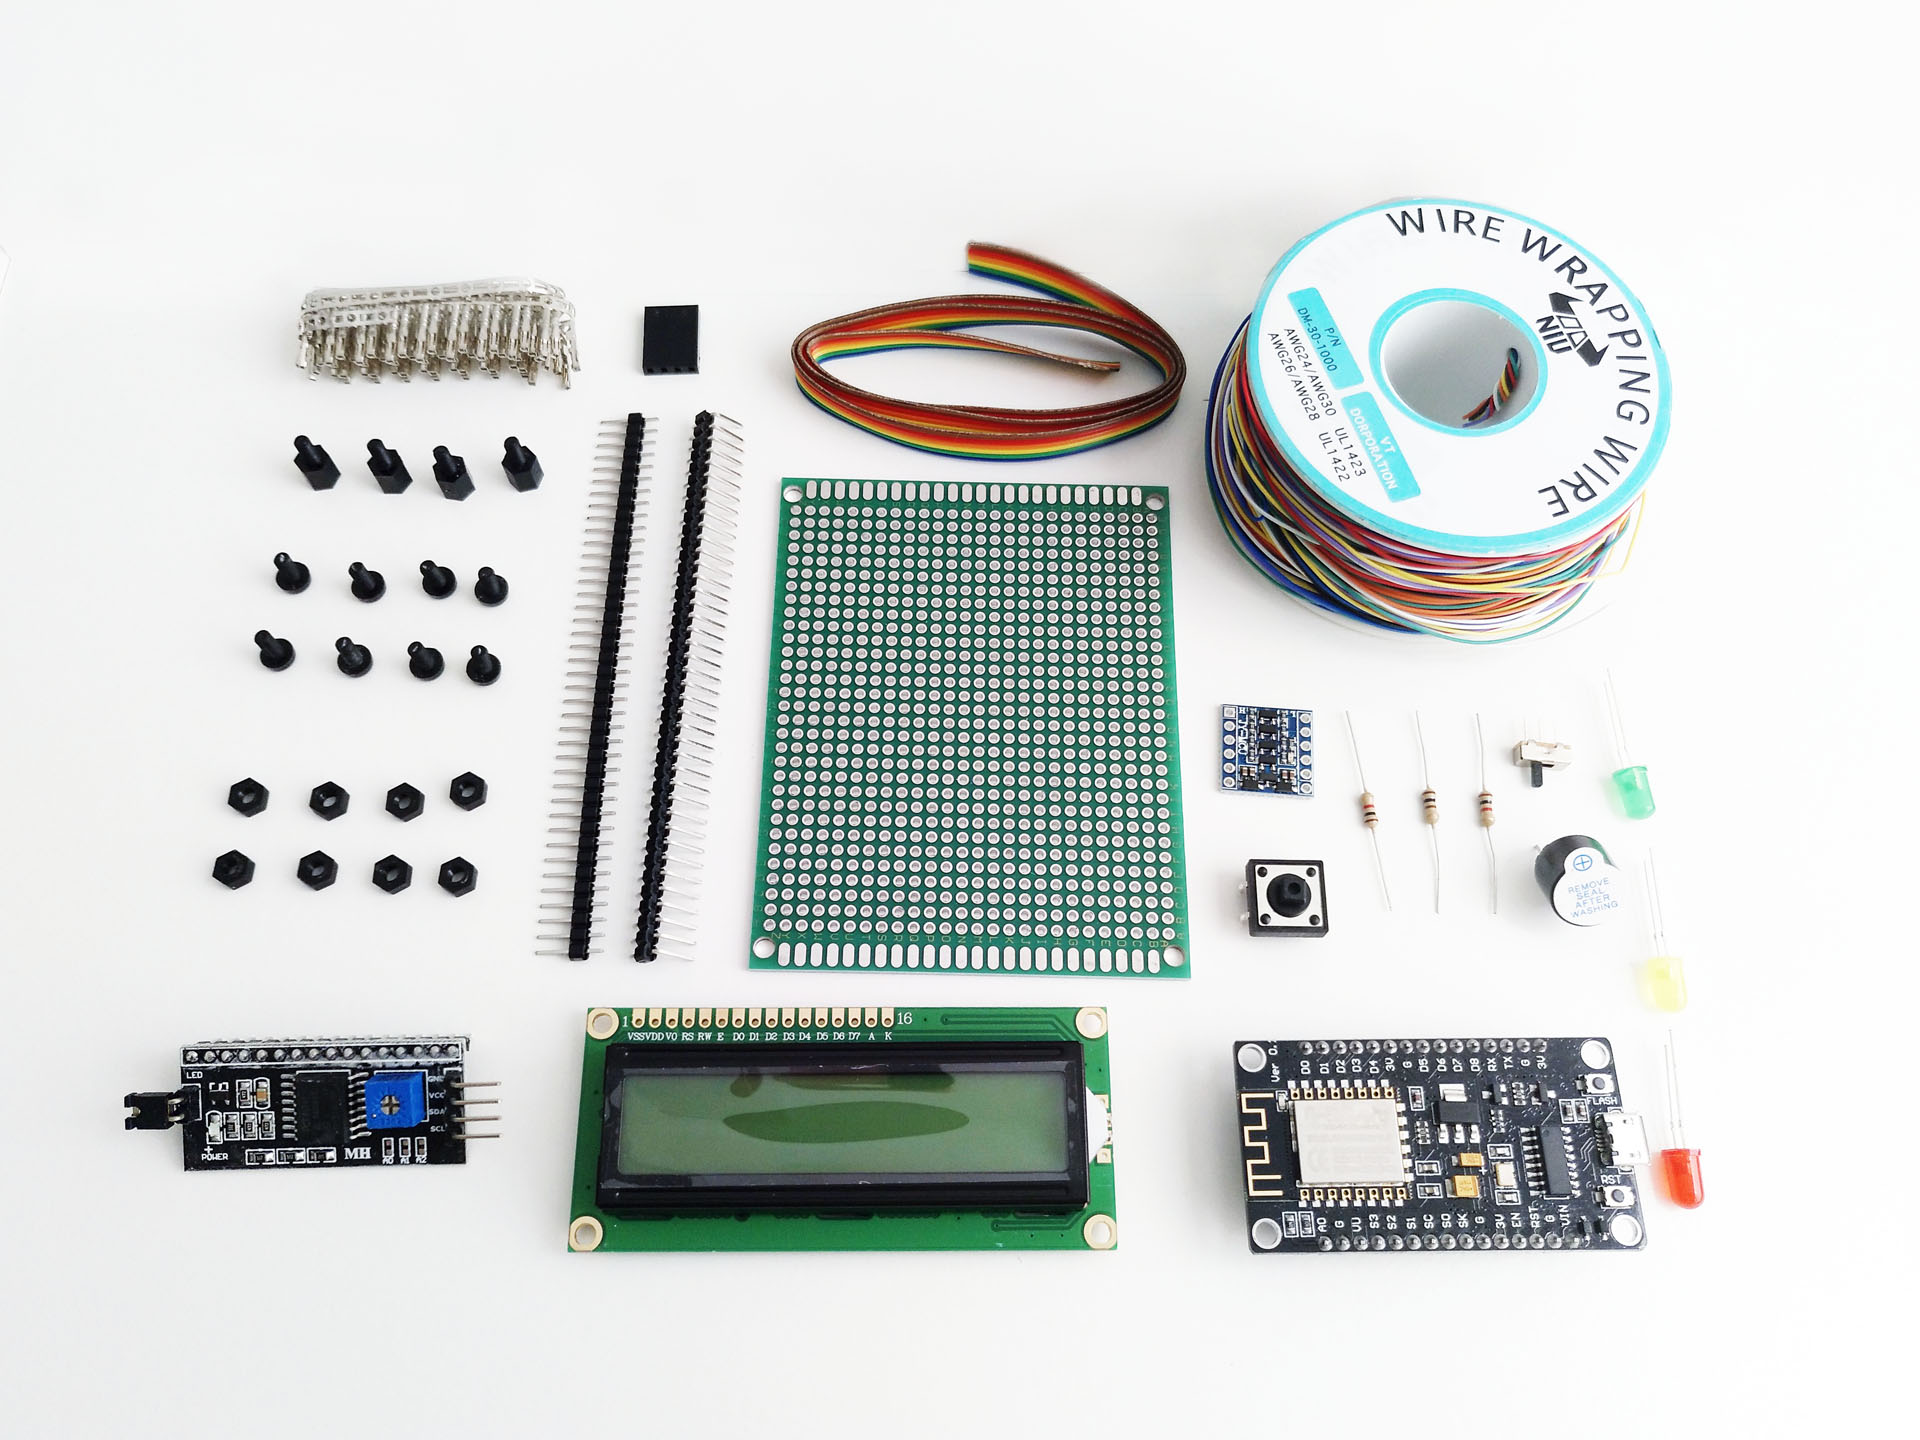
\includegraphics[width=0.98\columnwidth]{../photos/interior-pieces}
  \caption{Piezas para la construcción del módulo interior}
  \label{fig:interior-pieces}
\end{sidewaysfigure}

\clearpage

\subsection{Diseño de circuito impreso del módulo interior}

\vfill

\begin{figure}[H]
  \centering
  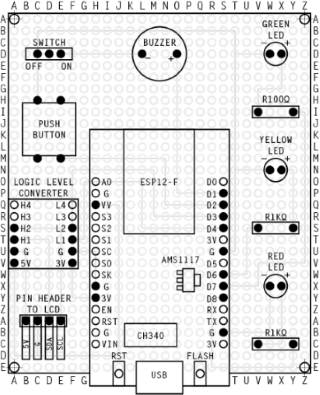
\includegraphics[width=0.7\columnwidth]{../design/interior-board-front}
  \caption{Diseño frontal de la placa de circuito impreso}
  \label{fig:interior-board-front}
\end{figure}

\vfill

\clearpage

\begin{figure}
  \centering
  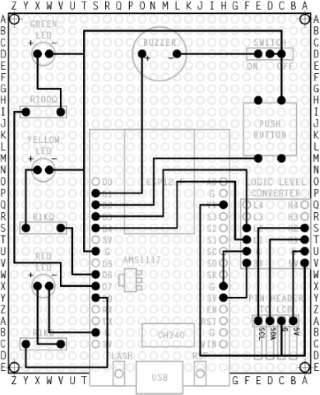
\includegraphics[width=0.7\columnwidth]{../design/interior-board-back}
  \caption{Diseño trasero de la placa de circuito impreso}
  \label{fig:interior-board-back}
\end{figure}

\clearpage

\subsection{Acabado final}

\vfill

\begin{figure}[H]
  \centering
  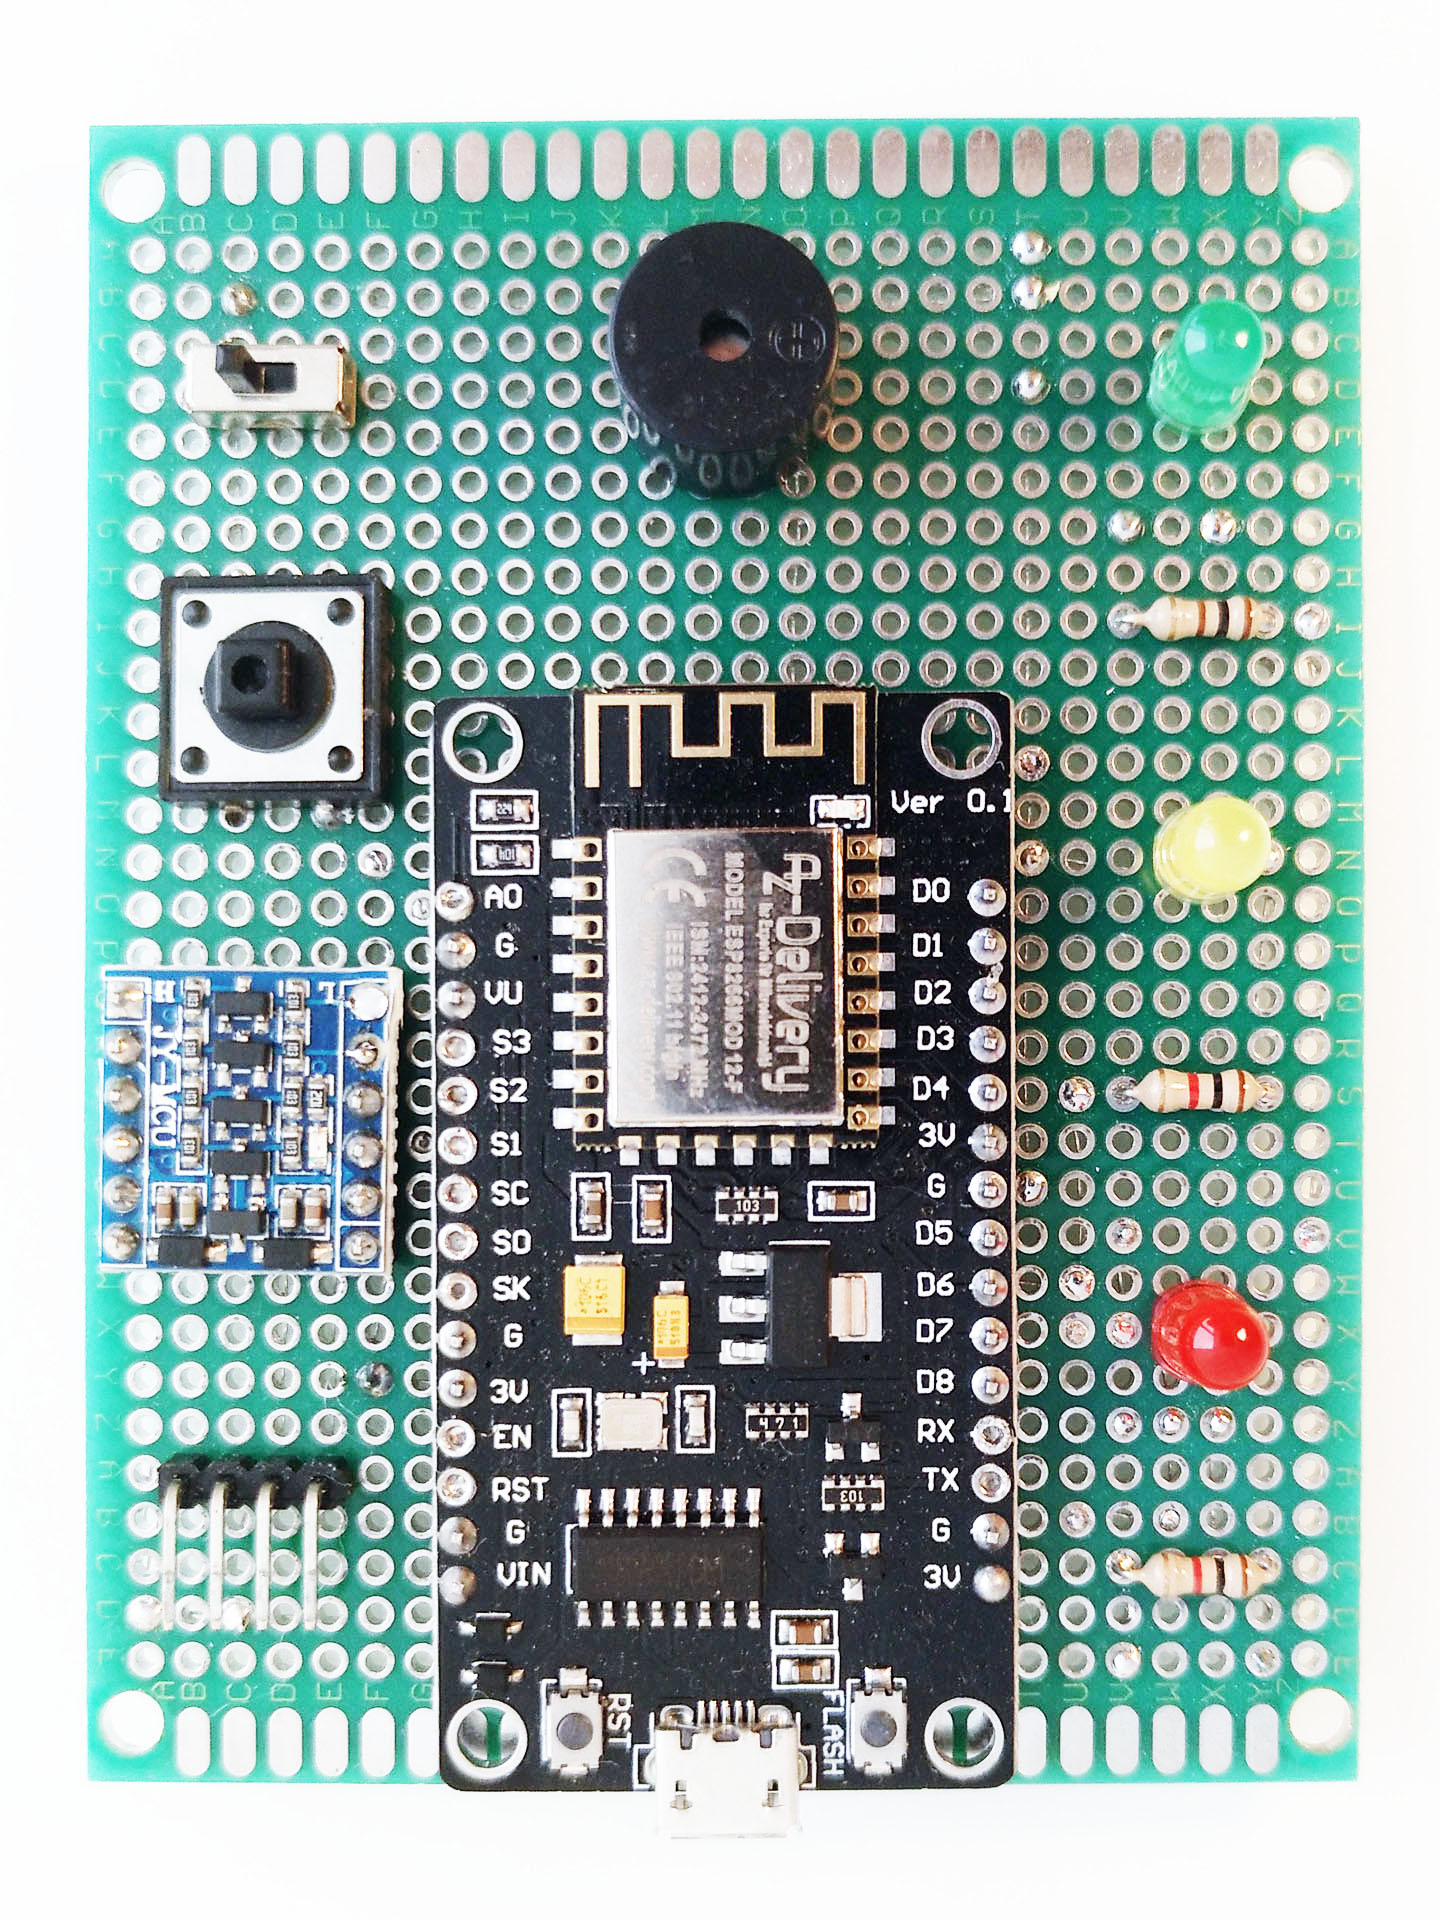
\includegraphics[width=0.7\columnwidth]{../photos/interior-pcb-front}
  \caption{Acabado final de la placa de circuito impreso (vista frontal)}
  \label{fig:interior-pcb-front}
\end{figure}

\vfill

\clearpage

\begin{figure}
  \centering
  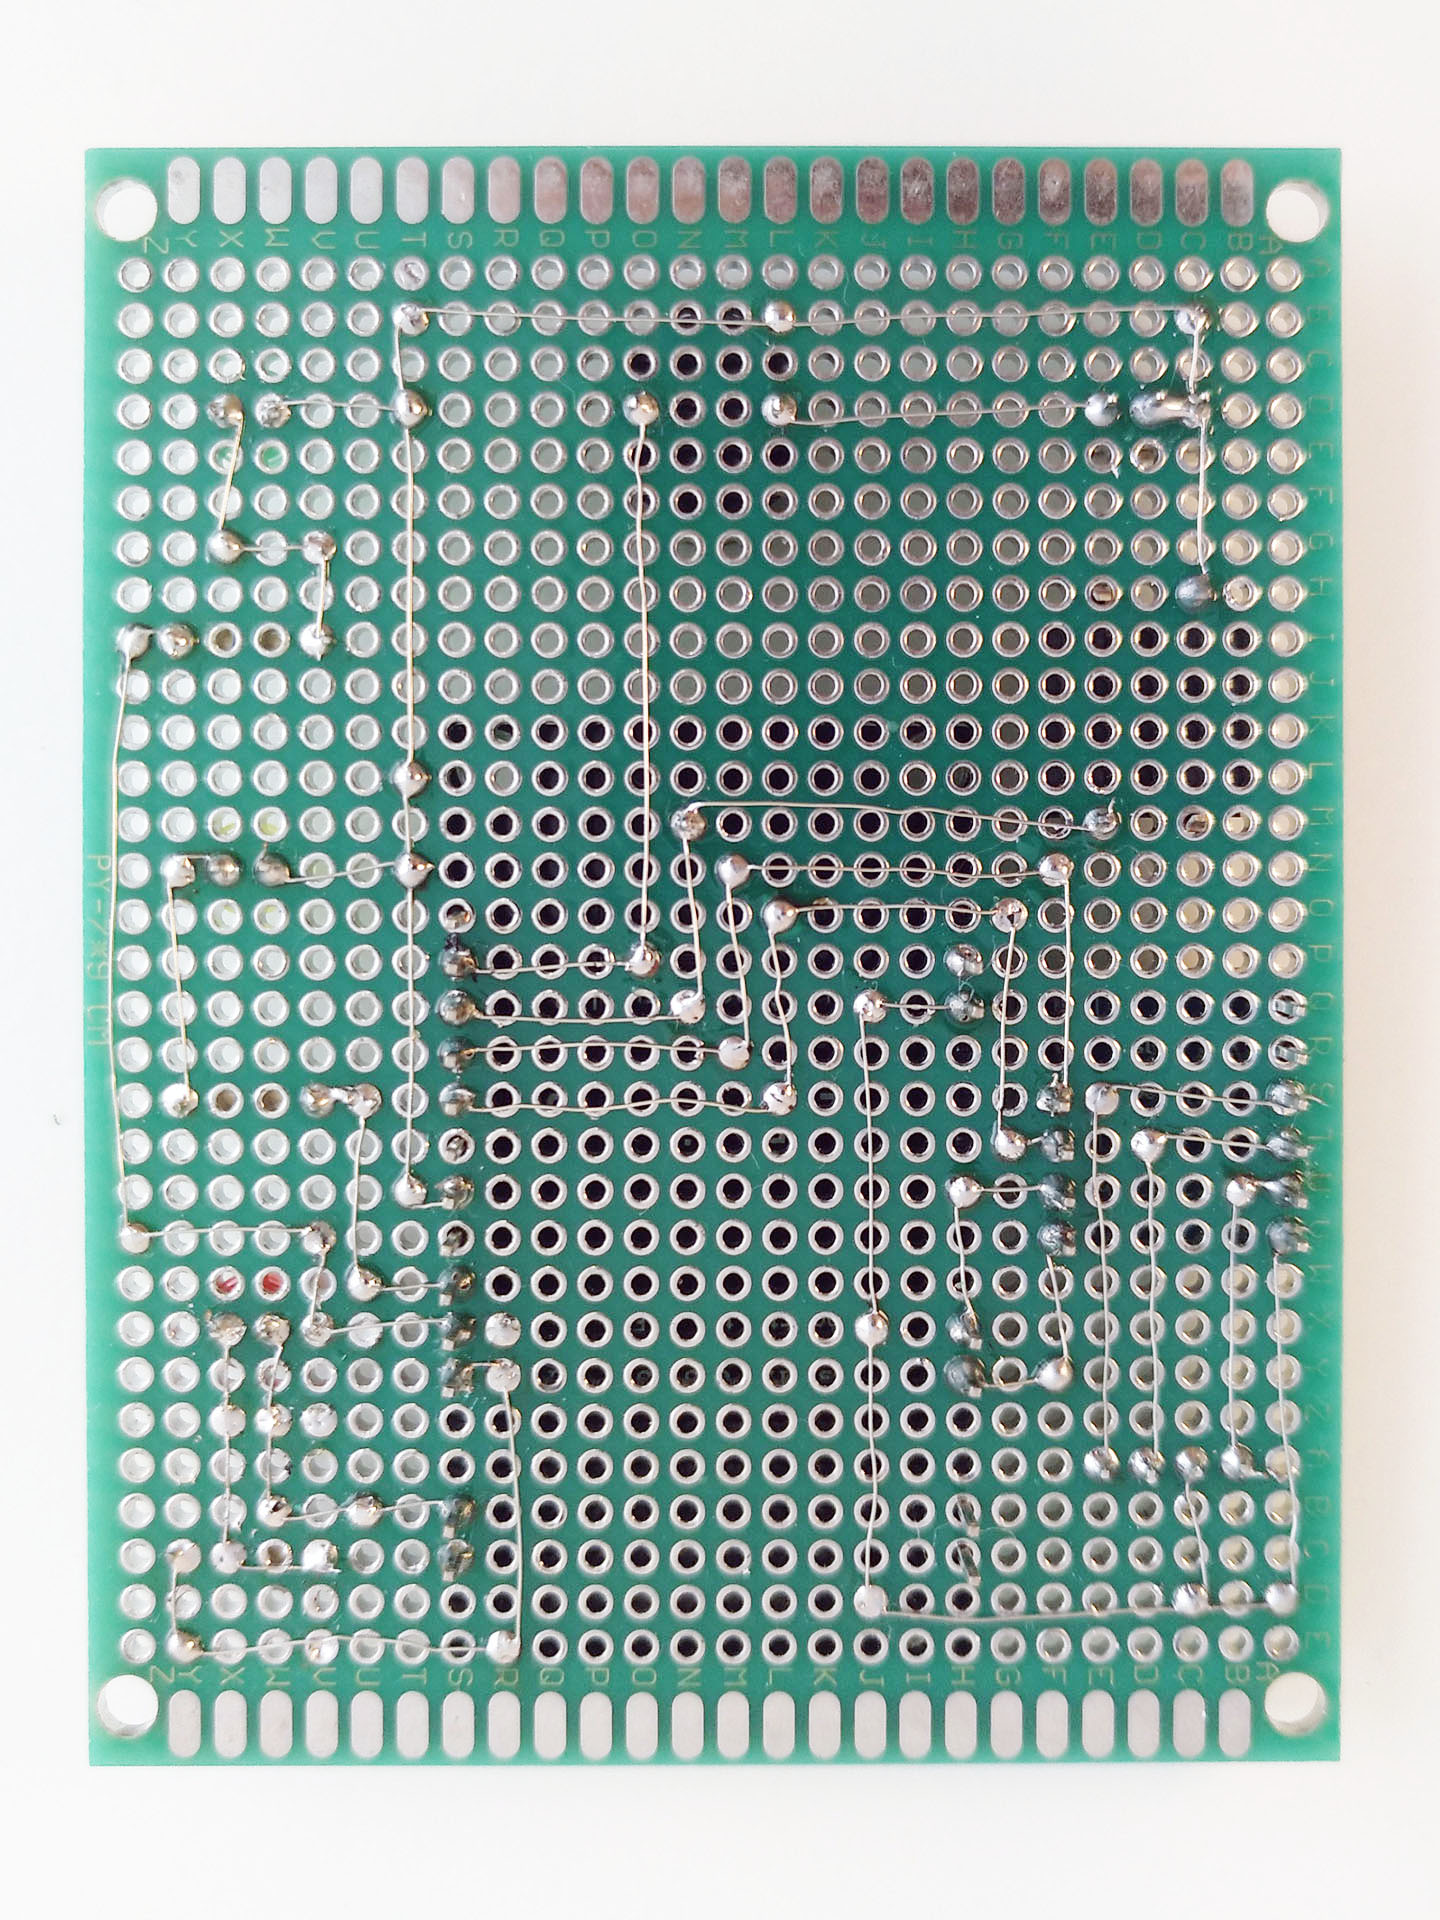
\includegraphics[width=0.7\columnwidth]{../photos/interior-pcb-back}
  \caption{Acabado final de la placa de circuito impreso (vista trasera)}
  \label{fig:interior-pcb-back}
\end{figure}

\clearpage


\section{Chasis del módulo interior}
\label{app:diseno-interior}

\subsection{Lista de materiales}

\vfill

\begin{table}[H]
\caption{Lista de materiales del módulo interior (chasis)}
\label{tab:materiales-carcasa-interior}
\begin{tabularx}{\textwidth}{cX}
\toprule
\headingc{Cantidad} & \headingc{Descripción} \\
\topruleb
1 & Hoja de metacrilato de 3mm de grosor (270mm x 90mm)\\*\midrule
8 & Tuercas de nylon M3 nylon hex nuts\\*\midrule
8 & Tornillos de nylon con cabeza Phillips M3 x 6mm\\*\midrule
4 & Tornillo de nylon con tuerca integrada M3 x 6mm + 6mm\\*\bottomrule
\end{tabularx}
\end{table}

\vfill

\subsection{Boceto del chasis del módulo interior}

\vfill

\begin{figure}[H]
  \centering
  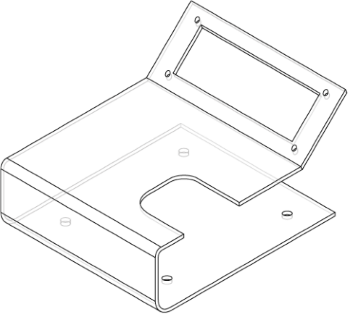
\includegraphics[width=0.53\columnwidth]{../design/interior-body-design}
  \caption{Boceto del chasis del módulo interior}
  \label{fig:interior-body-design}
\end{figure}

\vfill

\clearpage

\subsection{Mecanizado del chasis del módulo interior}

\vfill

\begin{figure}[H]
  \centering
  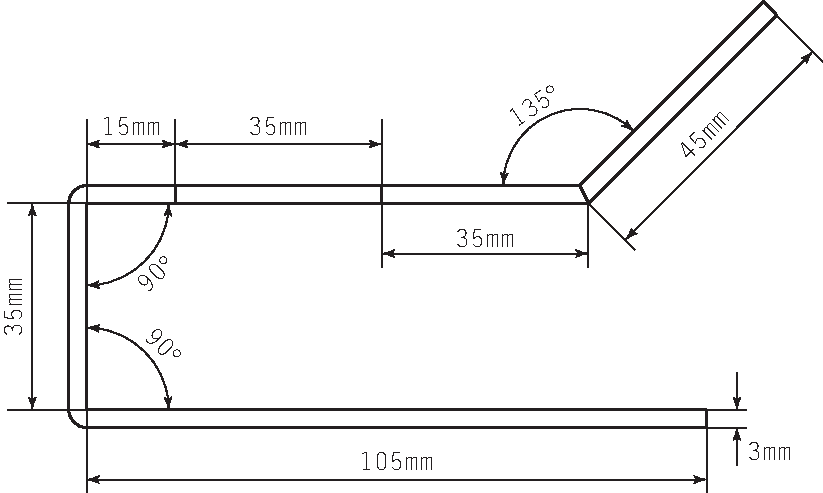
\includegraphics[width=0.8\columnwidth]{../design/interior-body-side}
  \caption{Doblado del chasis del módulo interior (vista lateral)}
  \label{fig:interior-body-side}
\end{figure}

\vfill

\clearpage

\begin{figure}
  \centering
  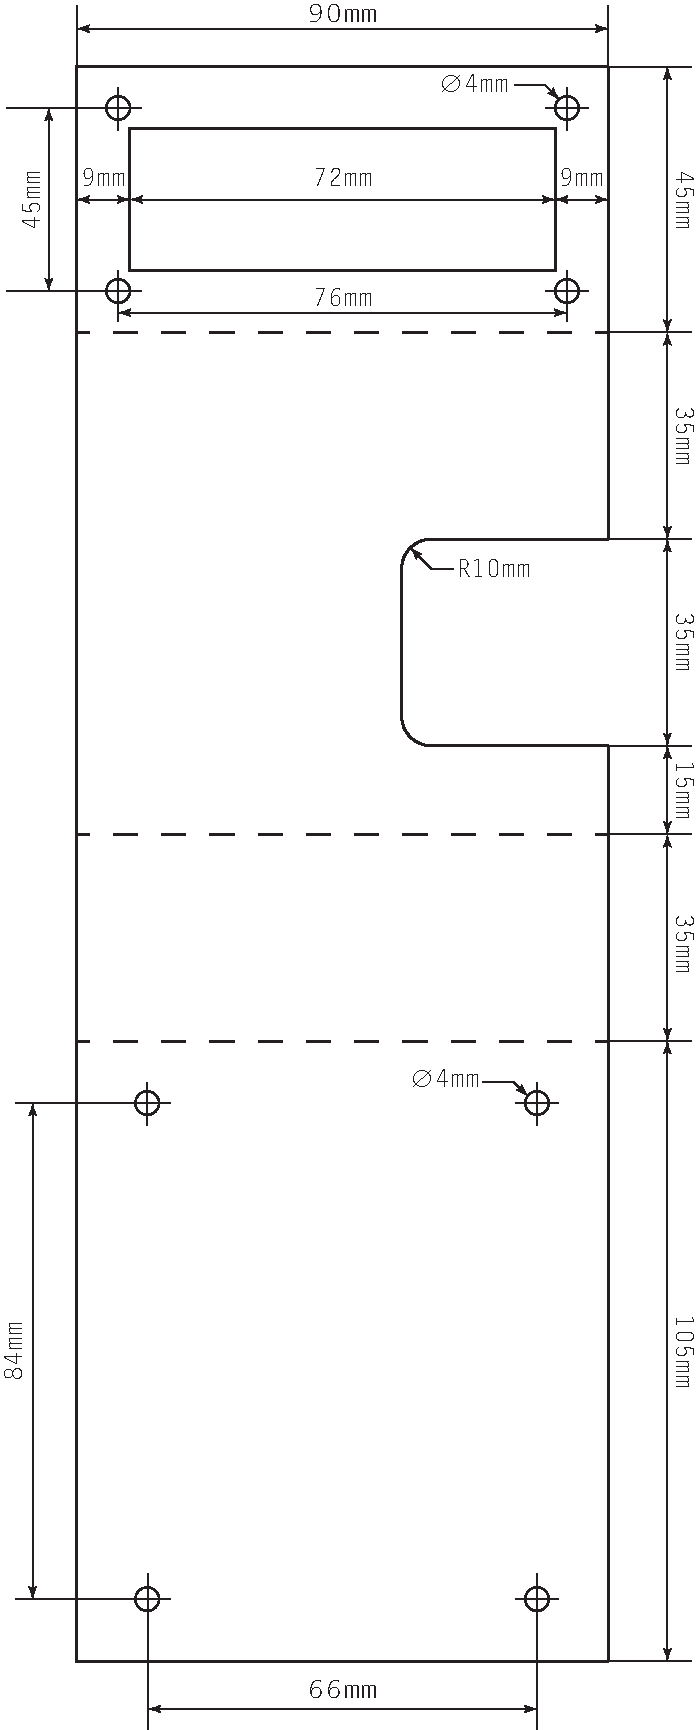
\includegraphics[height=0.98\textheight]{../design/interior-body-blueprint}
  \caption{Diseño del corte del chasis del módulo interior}
  \label{fig:interior-body-blueprint}
\end{figure}



\section{Placa de circuito impreso del módulo exterior}
\label{app:componentes-exterior}

\subsection{Lista de materiales}

\vfill

\begin{table}[H]
\caption{Lista de materiales del módulo exterior}
\label{tab:example}
\begin{tabularx}{\textwidth}{cX}
\toprule
\headingc{Cantidad} & \headingc{Descripción} \\
\topruleb
  1 & PCB de prototipado (70mm x 90mm)\\*\midrule
  1 & NodeMCU v3 (ESP8266)\\*\midrule
  1 & 1 sensor DHT22 (placa)\\*\midrule
  1 & Regulador de baja caída AP7361C-33ER-13\\*\midrule
  1 & Botón \textit{push} (normalmente abierto)\\*\midrule
  1 & Portabaterías 4 pilas AA \\*\midrule
  1 & Interruptor de flotador (normalmente cerrado)\\*\midrule
  1 & Resistencia 100 Ω \\*\midrule
  1 & Resistencia 220 Ω \\*\midrule
  1 & Interruptor de dos posiciones (3 pines)\\*\midrule
 -- & Pines variados\\*\midrule
 -- & Conectores Dupont variados\\*\midrule
 -- & Cables variados\\*\bottomrule
\end{tabularx}
\end{table}

\vfill

\clearpage

\begin{sidewaysfigure}
  \centering
  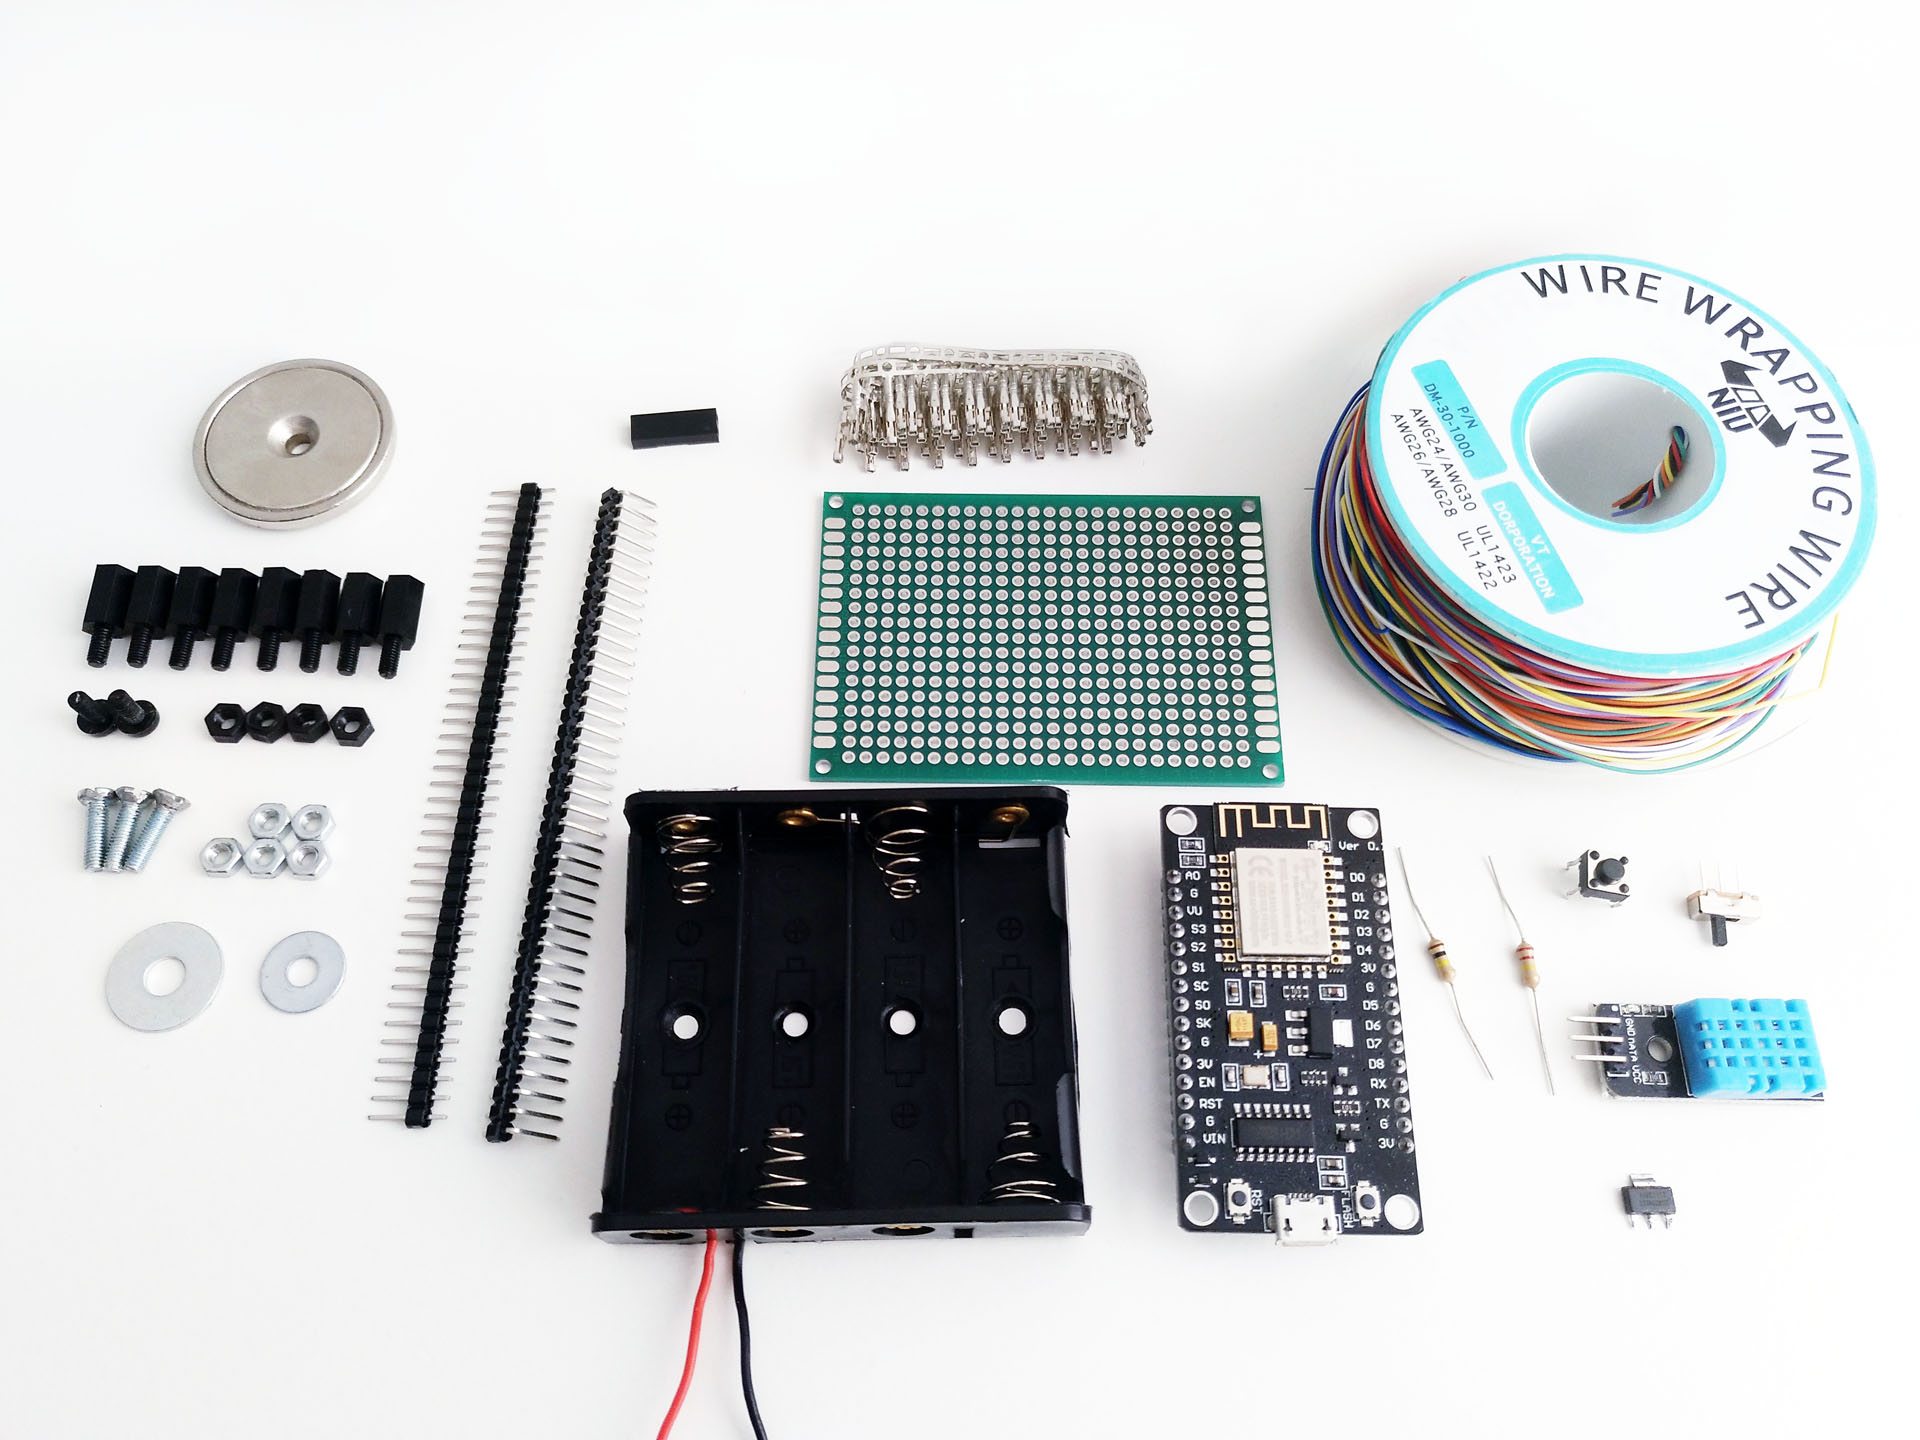
\includegraphics[width=0.98\columnwidth]{../photos/exterior-pieces}
  \caption{Piezas para la construcción del módulo exterior}
  \label{fig:exterior-pieces}
\end{sidewaysfigure}

\clearpage

\subsection{Diseño de circuito impreso del módulo exterior}

\vfill

\begin{figure}[H]
  \centering
  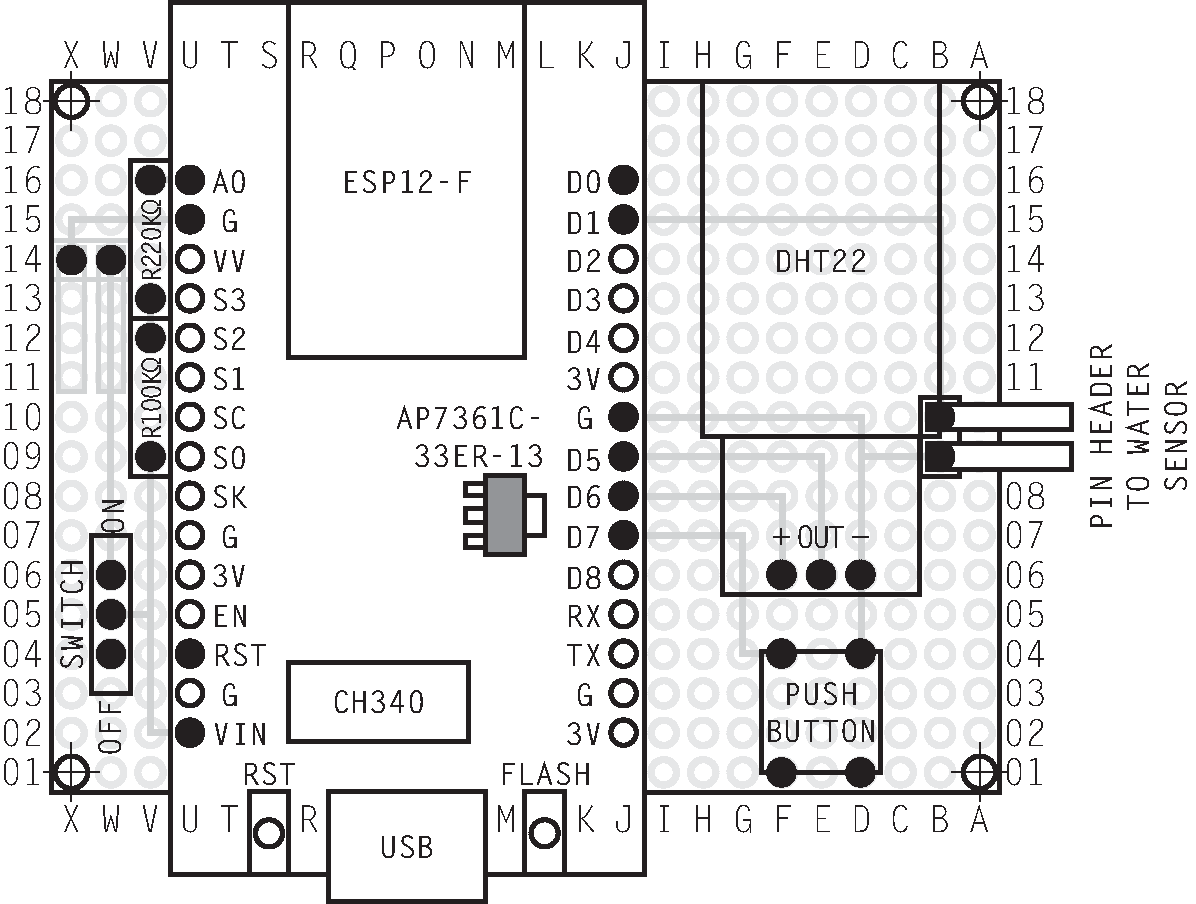
\includegraphics[width=1\columnwidth]{../design/exterior-board-front}
  \caption{Diseño frontal de la placa de circuito impreso}
  \label{fig:exterior-board-front}
\end{figure}

\vfill

\clearpage

\begin{figure}
  \centering
  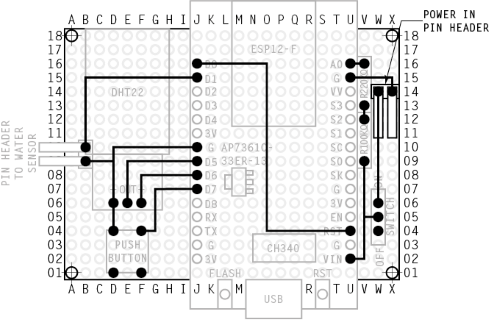
\includegraphics[width=1\columnwidth]{../design/exterior-board-back}
  \caption{Diseño trasero de la placa de circuito impreso}
  \label{fig:exterior-board-back}
\end{figure}

\clearpage

\subsection{Acabado final}

\vfill

\begin{figure}[H]
  \centering
  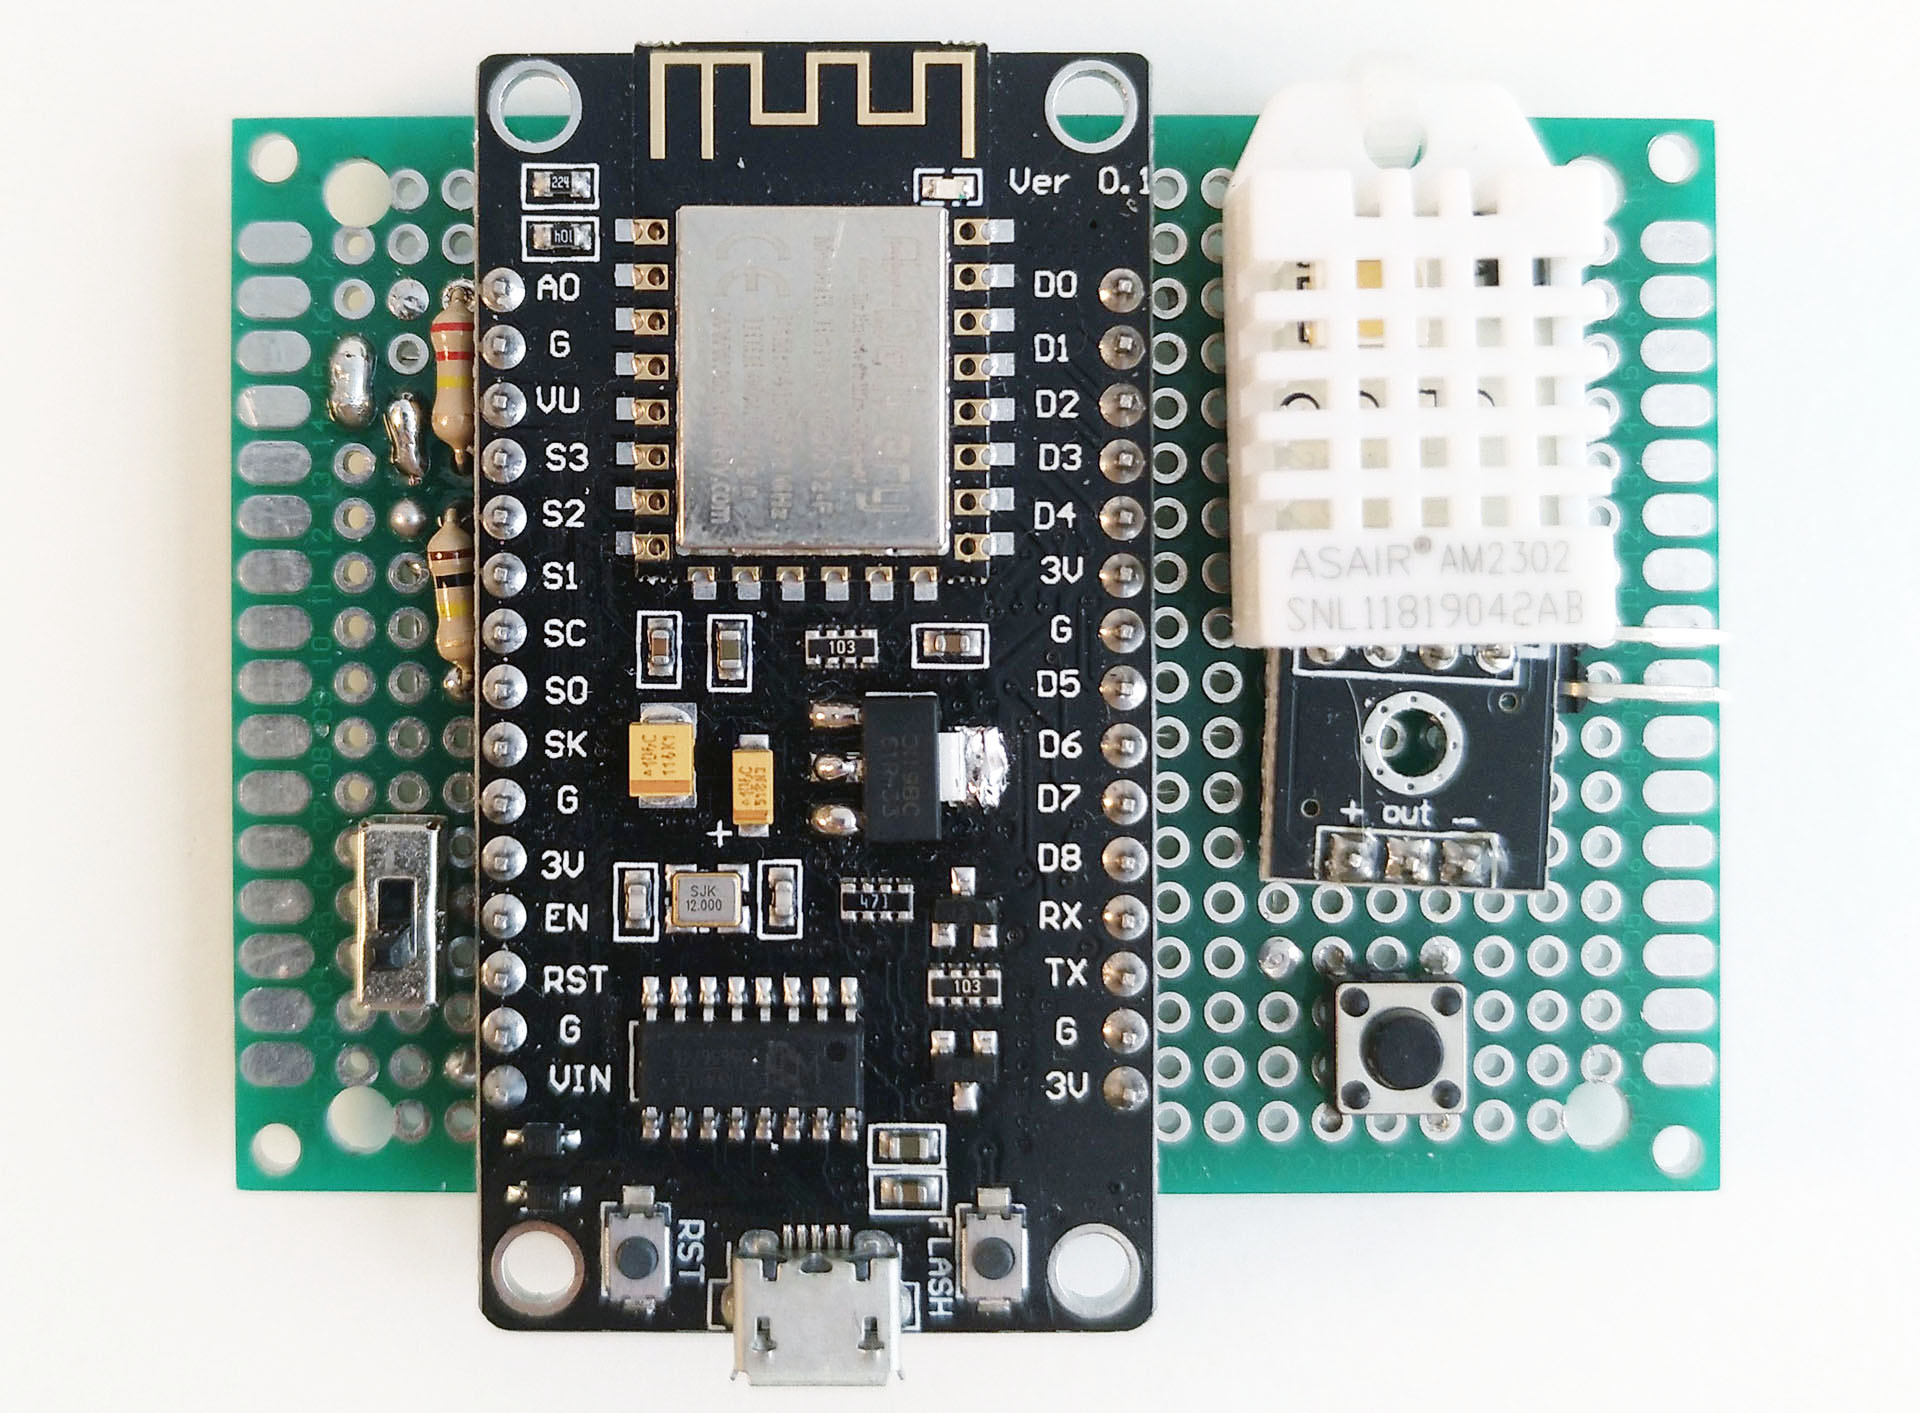
\includegraphics[width=1\columnwidth]{../photos/exterior-pcb-front}
  \caption{Acabado final de la placa de circuito impreso (vista frontal)}
  \label{fig:exterior-pcb-front}
\end{figure}

\vfill

\clearpage

\begin{figure}
  \centering
  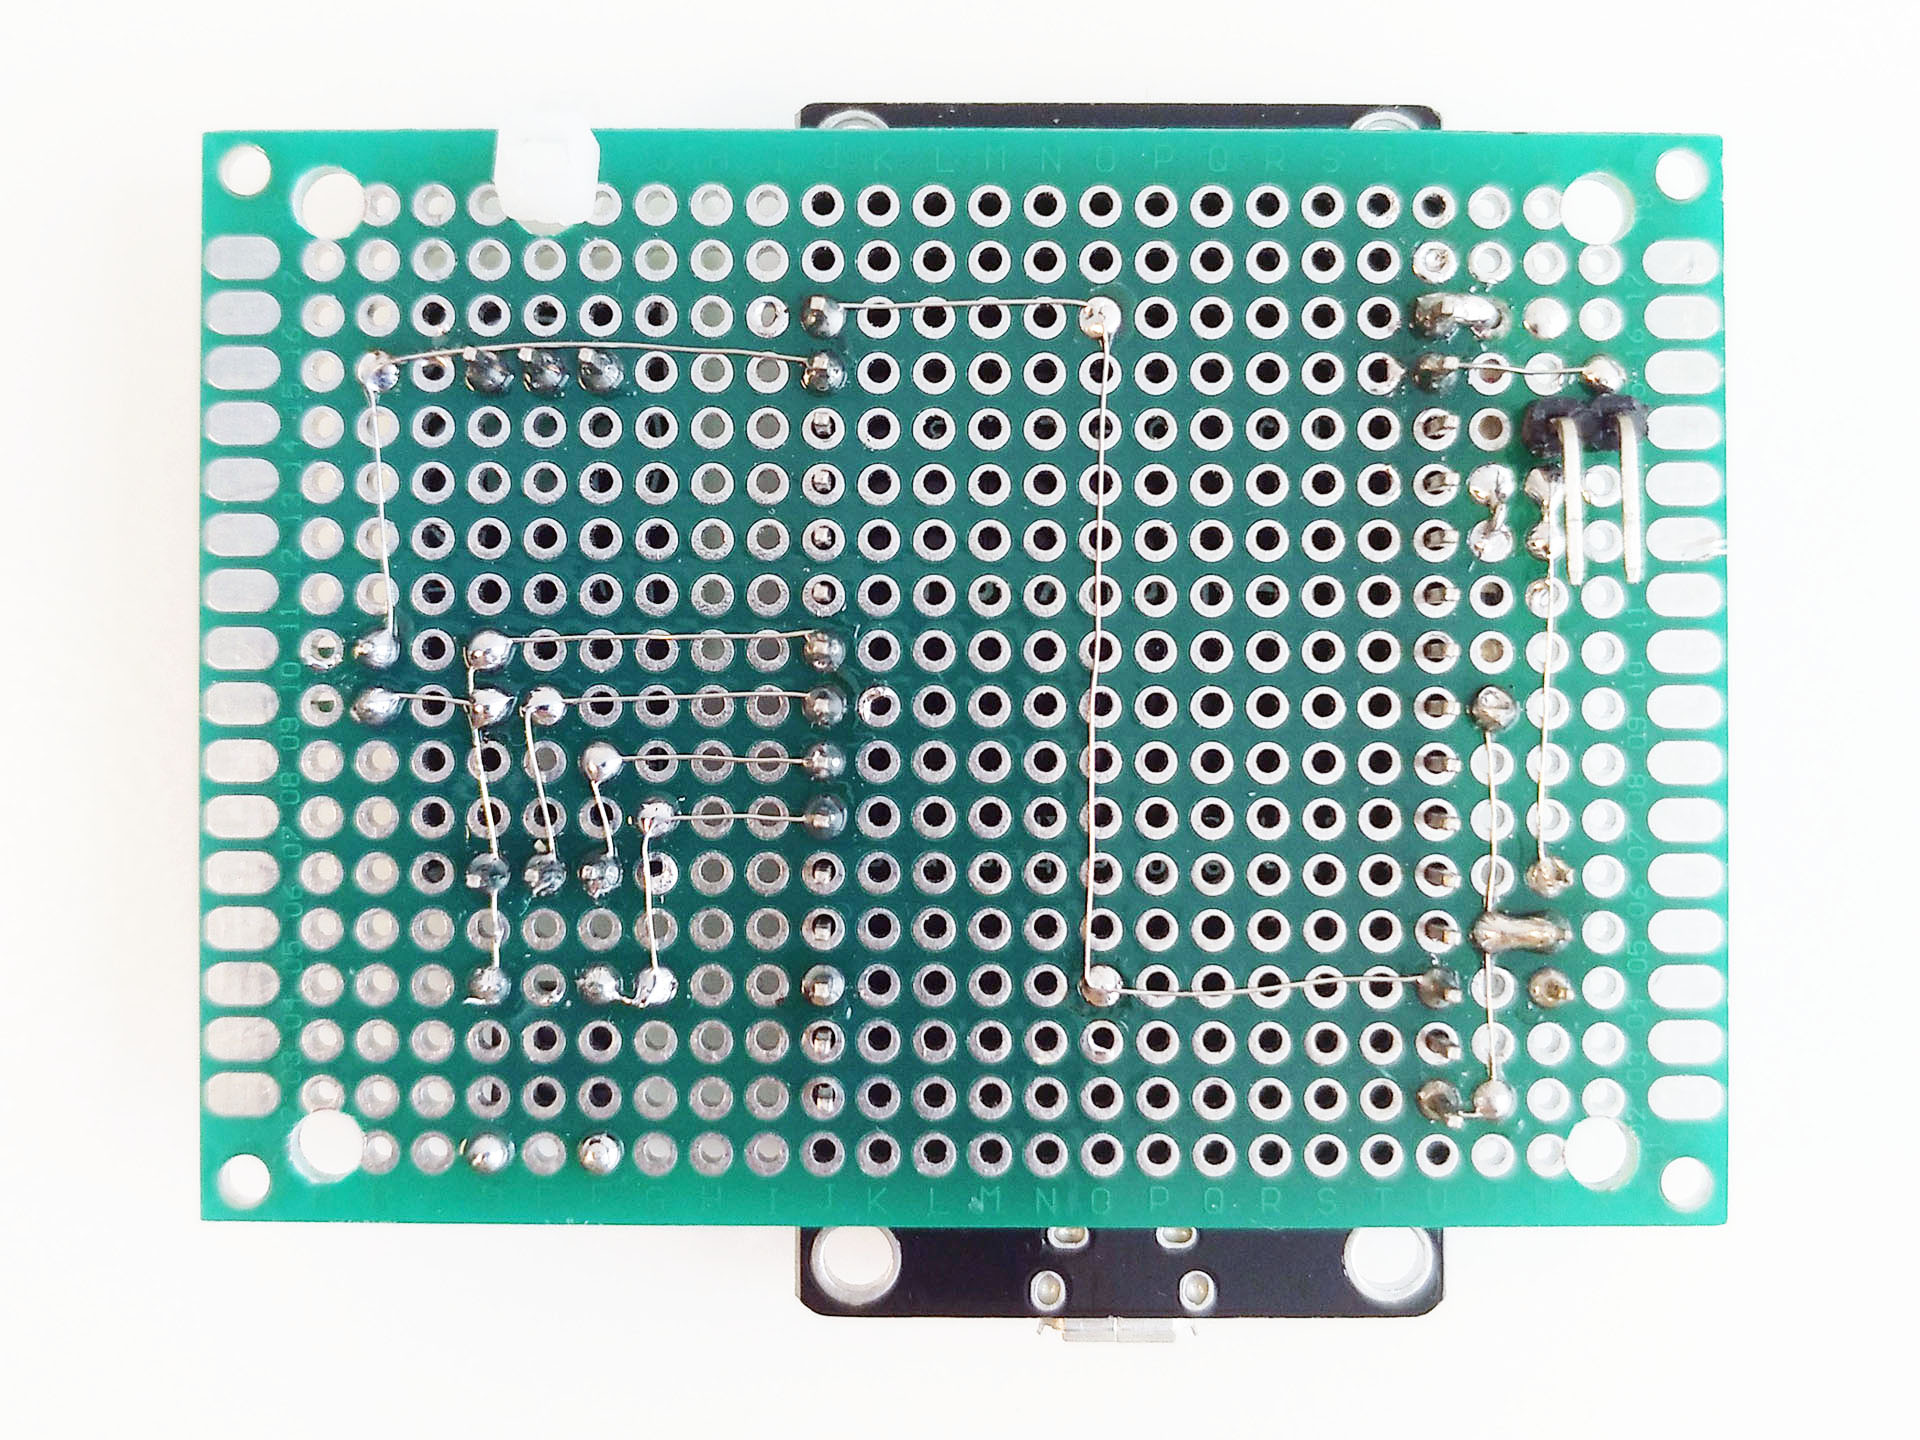
\includegraphics[width=1\columnwidth]{../photos/exterior-pcb-back}
  \caption{Acabado final de la placa de circuito impreso (vista trasera)}
  \label{fig:exterior-pcb-back}
\end{figure}

\clearpage


\section{Chasis y cubierta del módulo exterior}
\label{app:diseno-exterior}

\subsection{Lista de materiales}

\vfill

\begin{table}[H]
\caption{Lista de materiales del módulo exterior (chasis y cubierta)}
\label{tab:materiales-carcasa-exterior}
\begin{tabularx}{\textwidth}{cX}
\toprule
\headingc{Cantidad} & \headingc{Descripción} \\
\topruleb
 1 & Hoja de metacrilato de 3mm de grosor (105mm x 70mm)\\*\midrule
 1 & Hoja de metacrilato de 2mm de grosor (125mm x 115mm)\\*\midrule
 1 & Hoja de metacrilato de 2mm de grosor (170mm x 160mm)\\*\midrule
 4 & Tuercas de nylon M3 nylon\\*\midrule
 2 & Tornillos de nylon con cabeza Phillips M3 x 6mm\\*\midrule
 4 & Tornillo de nylon con tuerca integrada M3 x 6mm + 10mm\\*\midrule
 1 & Imán neodimio avellanado ($\diameter$30mm)\\*\midrule
 1 & Tornillo avellanado M3 x 10mm\\*\midrule
 2 & Tuercas de acero M3\\*\midrule
-- & Arandela(s)\\*\bottomrule
\end{tabularx}
\end{table}

\vfill

\subsection{Boceto del chasis del módulo exterior}

\vfill

\begin{figure}[H]
  \centering
  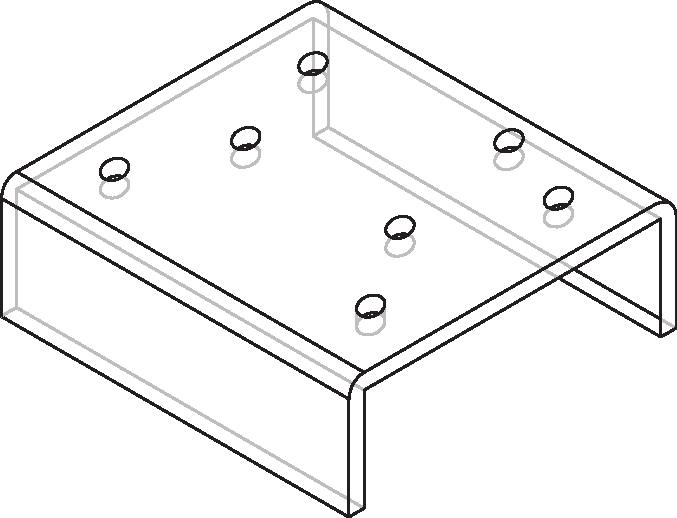
\includegraphics[width=0.6\columnwidth]{../design/exterior-skeleton-design}
  \caption{Boceto del chasis del módulo exterior}
  \label{fig:exterior-skeleton-design}
\end{figure}

\vfill

\subsection{Mecanizado del chasis del módulo exterior}

\vfill

\begin{figure}[H]
  \centering
  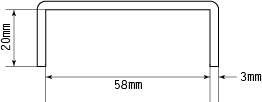
\includegraphics[width=0.8\columnwidth]{../design/exterior-skeleton-side}
  \caption{Doblado del chasis (vista lateral)}
  \label{fig:exterior-skeleton-side}
\end{figure}

\vfill

\clearpage

\begin{figure}
  \centering
  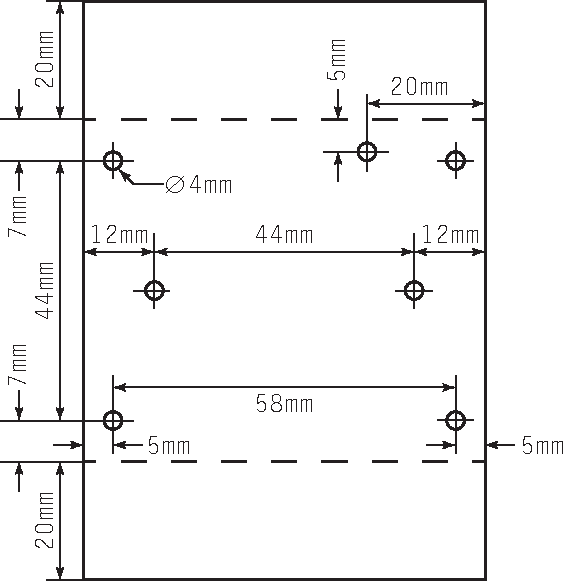
\includegraphics[height=0.8\columnwidth]{../design/exterior-skeleton-blueprint}
  \caption{Diseño del corte del chasis del módulo exterior}
  \label{fig:skeleton-skeleton-blueprint}
\end{figure}

\clearpage

\subsection{Boceto de la cubierta del módulo exterior}

\vfill

\begin{figure}[H]
  \centering
  \includegraphics[width=0.6\columnwidth]{../design/exterior-body-design}
  \caption{Boceto de la cubierta del módulo exterior}
  \label{fig:exterior-body-design}
\end{figure}

\vfill

\subsection{Mecanizado de la cubierta del módulo exterior}

\vfill

\begin{figure}[H]
  \centering
  \includegraphics[width=1\columnwidth]{../design/exterior-body-blueprint}
  \caption{Diseño del corte de la cubierta del módulo exterior (cuerpo principal)}
  \label{fig:exterior-body-blueprint}
\end{figure}

\vfill

\clearpage

\begin{figure}
  \centering
  \includegraphics[height=1\columnwidth]{../design/exterior-cover-blueprint}
  \caption{Diseño del corte de la cubierta del módulo exterior (tapa)}
  \label{fig:exterior-cover-blueprint}
\end{figure}




\section{Curva de descarga}
\label{app:curva-descarga}

La figura~\ref{fig:discharge-curve} muestra la curva de descarga de las baterías del \MEE cuando el \emph{Tiempo de espera entre mensajes} (ver Sección~\ref{sec:config}) se ha establecido en 1 minuto.
Con dicha frecuencia de mensajes, y con baterías en perfectas condiciones, el \ME tarda aproximadamente 18 días en alcanzar el umbral de batería bajo por defecto (4,72 V), y menos de 21 días en descargarse por completo. 

Dado el reducido consumo de batería del \MEE cuando se encuentra en reposo, es posible alargar la duración de las baterías de forma notable incrementando el \emph{Tiempo de espera entre mensajes} a varios minutos. Por ejemplo, con un tiempo de espera entre mensajes de 5 minutos la batería debería durar entre 10 y 12 semanas.

\begin{figure}[H]
  \centering
  \includegraphics[width=1\columnwidth]{images/discharge-curve}
  \caption{Curva de descarga}
  \label{fig:discharge-curve}
\end{figure}


\section{MQTT Topics}
\label{app:mqtt-topics}

La tabla~\ref{tab:topics} resume los \emph{topics} publicados por el \MEE que son reconocidos por el \MIE.
Es posible conectarse conectarse al \MIE y suscribirse a los \emph{topics} abajo listados empleando un cliente MQTT para recibir la información publicada por el \MEE en otros dispositivos (como por ejemplo, un teléfono móvil).

\begin{table}[H]
\renewcommand\tabularxcolumn[1]{m{#1}}
\caption{\textit{Topics} empleados en el \textit{Chana Monitoring System}}
\label{tab:topics}
\begin{tabularx}{\textwidth}{lcX}
\toprule
\headingc{Topic} & \headingc{Tipo} & \headingc{Descripción} \\
\topruleb
  \verb|chanams/deposit-full| & \verb|boolean| & Valor lógico que indica si el depósito monitorizado por el \ME está lleno. \\*\midrule
  \verb|chanams/battery-vcc|  & \verb|float|   & Valor numérico que indica el voltaje que es capaz de proporcionar la batería del \ME en voltios. \\*\midrule
  \verb|chanams/temperature|  & \verb|float|   & Valor numérico que indica la temperatura exterior detectada por el \ME. \\*\midrule
  \verb|chanams/humidity|     & \verb|float|   & Valor numérico que indica la humedad relativa del aire detectada por el \ME. \\*\midrule
  \verb|chanams/heat-index|   & \verb|float|   & Valor numérico que indica la sensación térmica en el exterior. Se calcula a partir de los valores de temperatura y humedad detectados por el \ME. Sin uso en el \MI. \\*\bottomrule
\end{tabularx}
\end{table}

\cleardoublepage

% % Biliography
% %%%%%%%%%%%%%%%%%%%%%%%%%%%%%%%%%%%%%%%%%%%%%%%%%%%%%%%%%%%%%%%%%%%%%%
% 
% \cleardoublepage
% \bibliographystyle{plain}
% \bibliography{bib/bibliography}
% 
% % Clarifications
% %%%%%%%%%%%%%%%%%%%%%%%%%%%%%%%%%%%%%%%%%%%%%%%%%%%%%%%%%%%%%%%%%%%%%%
% 
% % Print them only if the notes package is loaded (c@pagenode exists)
% % and there are notes defined within the document (pnotesavechap > 0)
% 
% \makeatletter
% \ifcsname c@pagenote\endcsname
% \ifthenelse{\value{pnotesavechap}>0}{\cleardoublepage\printnotes}{}
% \fi
% \makeatother


\makeback

\end{document}          
